% !TeX program = xelatex
%% ============================================================
%% Modélisation Prédictive Hybride par Géostatistique et Apprentissage Automatique
%% des Paramètres Géotechniques Nationaux : Application au Togo
%% Structure IMRaD — version 2026-06-02
%% ============================================================
\documentclass[10pt,a4paper,twocolumn]{article}

\usepackage[a4paper,top=2.2cm,bottom=2.2cm,left=1.5cm,right=1.5cm,columnsep=0.8cm]{geometry}
\usepackage[french]{babel}
\usepackage{csquotes}
\usepackage{graphicx}
\usepackage{amsmath,amssymb,amsfonts}
\usepackage{bm}
\usepackage{microtype}
\usepackage{titlesec}
\usepackage{caption}
\usepackage{subcaption}
\usepackage{booktabs}
\usepackage{array}
\usepackage{multirow}
\usepackage{placeins}
\usepackage{afterpage}
\usepackage{xcolor}
\usepackage{enumitem}
\usepackage{hyperref}
\hypersetup{hidelinks}
\usepackage{fontspec}
\usepackage{newtxmath}
\usepackage[style=ieee,backend=biber]{biblatex}
\addbibresource{bibliographie.bib}

\IfFontExistsTF{Times New Roman}{
  \setmainfont{Times New Roman}
}{\setmainfont{TeX Gyre Termes}}

%% Mise en page sections — sous-titres H3 et inférieurs en italique
\titleformat{\section}{\normalfont\fontsize{11}{13}\bfseries}{\thesection.}{0.8em}{}
\titleformat{\subsection}{\normalfont\fontsize{10}{12}\bfseries}{\thesubsection}{0.8em}{}
\titleformat{\subsubsection}{\normalfont\fontsize{10}{12}\itshape}{\thesubsubsection}{0.6em}{}
\titlespacing{\section}{0pt}{8pt}{4pt}
\titlespacing{\subsection}{0pt}{6pt}{3pt}
\titlespacing{\subsubsection}{0pt}{4pt}{2pt}

%% Légendes
\captionsetup{font=small, labelfont=bf, labelsep=endash, justification=justified}

%% Commandes mathématiques
\newcommand{\bZ}{\mathbf{Z}}
\newcommand{\bx}{\mathbf{x}}
\newcommand{\bs}{\mathbf{s}}
\newcommand{\bK}{\mathbf{K}}
\newcommand{\blambda}{\boldsymbol{\lambda}}
\newcommand{\bSigma}{\boldsymbol{\Sigma}}
\newcommand{\KED}{\text{KED-H}}
\newcommand{\RK}{\text{RK-SCORPAN}}
\newcommand{\BLUP}{\text{BLUP}}

%% Titre
\title{%
  \vspace{-1.4cm}%
  \fontsize{13}{15}\bfseries%
  MODÉLISATION PRÉDICTIVE HYBRIDE PAR GÉOSTATISTIQUE\\
  ET APPRENTISSAGE AUTOMATIQUE DES PARAMÈTRES\\
  GÉOTECHNIQUES NATIONAUX : APPLICATION AU TOGO\\[4pt]
  {\fontsize{10.5}{13}\normalfont\itshape
    Krigeage Hiérarchique 5 Niveaux, Régression SCORPAN, Fusion Bayésienne,
    Télédétection Sentinel-2, Processus Gaussien Multi-Tâches\\
    (56\,600~km², 573~sondages, 11~paramètres, 29\,407~mailles)}%
}

\author{%
  \fontsize{10}{12}\normalfont
  Serge TABE DJATO\textsuperscript{1*}\\[3pt]
  \fontsize{9}{11}\normalfont
  \textsuperscript{1}Institut des Sciences Technologiques Économiques et Administratives
  (FORMATEC), Lomé, Togo.\\
  \textsuperscript{*}Correspondance : \texttt{serge.tdjato@gmail.com}
}
\date{}

\begin{document}

\twocolumn[%
  \maketitle
  \vspace{-0.5cm}
  \rule{\linewidth}{0.4pt}
  \vspace{0.15cm}

  \noindent\small
  \textbf{Résumé ---} \textit{%
    La cartographie géotechnique à l'échelle nationale pose un défi fondamental
    de densité : 573~sondages pour 56\,600~km\textsuperscript{2} de territoire togolais.
    Cet article présente une hiérarchie L1--L4 de modèles géostatistiques et
    d'apprentissage automatique interpolant onze paramètres géotechniques
    (VBS, IP, WL, WP, EG, Rd, CBR\,95\%, $\gamma_d$, $w_{\mathrm{opt}}$, $E_m$, $P_l$)
    sur 29\,407~mailles (2~km~$\times$~2~km).
    Le Krigeage avec Dérive Hiérarchique 5 niveaux (KED-H, L1) intègre les couches
    géologiques, pédologiques et géomorphologiques togolaises,
    atteignant LOO-RMSE(VBS, H1)~=~3{,}147~g/100g ($n=113$),
    LOO-RMSE(CBR\,95\%, H1)~=~16{,}14\,\%~($n=117$),
    LOO-RMSE(Rd, H1)~=~3{,}45~MPa ($n=89$) et
    LOO-RMSE($\gamma_d$, H1)~=~1{,}41~kN/m³ ($n=318$).
    La Régression Kriging SCORPAN (RK, L2a) atteint LOO-RMSE(VBS)~=~2{,}625~g/100g.
    Une Fusion Bayésienne BLUP (L2b) réduit la variance de krigeage de
    47{,}9\,\%~$\pm$~1{,}5\,\% (propriété mathématiquement certifiée).
    Un modèle PLS sur indices spectraux Sentinel-2 (VfS, L3,
    LOO-RMSE~=~2{,}788~g/100g~$<$~KED-H) et un Processus Gaussien
    Multi-Tâches (MTGP/ICM, L4, $r_{\mathrm{IP,WL}}=0{,}773$) complètent
    la hiérarchie. Le système produit 441\,105~valeurs interpolées
    avec intervalles de confiance à 95\% et constitue le premier atlas
    géotechnique national à haute résolution du Togo.%
  }

  \smallskip
  \noindent\small
  \textbf{Abstract ---} \textit{%
    National-scale geotechnical mapping faces a fundamental data density challenge:
    573~boreholes over 56\,600~km\textsuperscript{2}.
    A four-level hierarchy (L1--L4) of geostatistical and machine learning models
    interpolates eleven parameters (VBS, IP, WL, WP, EG, Rd, CBR\,95\%,
    $\gamma_d$, $w_{\mathrm{opt}}$, $E_m$, $P_l$) over 29,407~cells.
    Hierarchical External Drift Kriging (KED-H, L1) achieves
    LOO-RMSE(VBS,H1)~=~3.147~g/100g ($n=113$),
    LOO-RMSE(CBR\,95\%,H1)~=~16.14\,\% ($n=117$) and
    LOO-RMSE(Rd,H1)~=~3.45~MPa ($n=89$).
    SCORPAN Regression Kriging (RK, L2a) achieves 2.625~g/100g for VBS.
    Bayesian BLUP fusion (L2b) reduces kriging variance by 47.9\,\%~$\pm$~1.5\,\%.
    Sentinel-2 PLS (VfS, L3) yields 2.788~g/100g~$<$~KED-H,
    establishing a proof of concept for laboratory-free geotechnics.%
  }

  \smallskip
  \noindent\small
  \textbf{Mots clés :} Krigeage Externe Hiérarchique, SCORPAN, Fusion Bayésienne,
    MTGP/ICM, CBR, Pénétromètre, Géotechnique, Togo.

  \vspace{0.15cm}
  \rule{\linewidth}{0.4pt}
  \vspace{0.3cm}
]

% ══════════════════════════════════════════════════════════════════════════════
\section{Introduction}
% ══════════════════════════════════════════════════════════════════════════════

\subsection{Contexte et problématique}

La planification des infrastructures civiles en Afrique subsaharienne repose
quasi-exclusivement sur des campagnes géotechniques ponctuelles dont la densité
spatiale est incompatible avec les exigences du dimensionnement distribué.
Au Togo, les paramètres fondamentaux --- Valeur au Bleu de Méthylène (VBS),
Indice de Plasticité (IP), Limites d'Atterberg (WL, WP), Coefficient de Gonflement
(EG), CBR~95\% Proctor, densité sèche optimale ($\gamma_d$), teneur en eau
optimale ($w_{\mathrm{opt}}$), résistance dynamique Rd, et paramètres
pressiométriques ($E_m$, $P_l$) --- sont disponibles sur 573~sondages
géoréférencés pour un territoire de 56\,600~km²
($\rho \approx 1{,}01 \times 10^{-2}$~sondage~km$^{-2}$)
\cite{mcbratney2003digital}.

La transformation de cette information lacunaire en une surface de prédiction
continue est un problème inverse classiquement résolu par géostatistique.
Les travaux de Matheron \cite{matheron1963} ont établi le Krigeage Ordinaire
comme estimateur MVUE. Le Krigeage avec Dérive Externe (KED) \cite{odeh1994further}
incorpore une variable auxiliaire continue, tandis que la Régression Kriging (RK)
\cite{hengl2007regression} sépare explicitement la tendance déterministe
des résidus stochastiques.

Dans le contexte togolais, ces méthodes présentent deux limites structurelles :
(i)~les couches géologiques disponibles (pédologie, risque RGA, géologie)
offrent une information catégorielle multi-échelle non exploitée ;
(ii)~les cinq paramètres d'argilosité sont fortement corrélés
($r_{\mathrm{IP,WL}} = 0{,}773$, $r_{\mathrm{IP,EG}} = 0{,}721$) ---
leur modélisation indépendante gaspille une information inter-paramètre
substantielle.

Cet article présente une hiérarchie L1--L4 répondant à ces limites :
(L1)~KED avec Dérive Hiérarchique 5 niveaux (KED-H),
(L2a)~Régression Kriging SCORPAN (RK-SCORPAN),
(L2b)~Fusion Bayésienne BLUP,
(L3)~Régression PLS sur indices Sentinel-2 (VfS-PLS),
(L4)~Processus Gaussien Multi-Tâches (MTGP/ICM).
La section~\ref{sec:methodes} détaille données et modèles ;
la section~\ref{sec:resultats} présente les performances ;
la section~\ref{sec:discussion} discute les résultats ;
la section~\ref{sec:conclusion} conclut.

\subsection{Rappels théoriques sur la géostatistique linéaire}
\label{sec:theorie}

\subsubsection{Hypothèses de stationnarité}

Le cadre géostatistique repose sur la stationnarité d'ordre~2 :
$\mathbb{E}[Z(\bs)] = m(\bs)$,
$\mathrm{Cov}[Z(\bs), Z(\bs')] = C(\bs - \bs')$.
Le semi-variogramme intrinsèque
$\gamma(\mathbf{h}) = \frac{1}{2}\mathrm{Var}[Z(\bs+\mathbf{h})-Z(\bs)]$
est moins restrictif et s'applique aux processus à variance infinie.
Dans nos données, la stationnarité est satisfaite après déduction de la dérive
hiérarchique $\mu_h(\bs)$~\eqref{eq:prior_hierarchique}.

\subsubsection{Propriétés d'optimalité du krigeage}

L'estimateur $Z^* = \sum_i \lambda_i z(\bs_i)$ est optimal (MVUE) dans la
classe des estimateurs linéaires non-biaisés, garantissant
linéarité, non-biais et variance minimale simultanément.
Cette optimalité est conditionnelle au modèle de covariance, ce qui motive
l'analyse de sensibilité (section~\ref{subsec:sensibilite}).

\subsubsection{Intervalles de prédiction}

La variance de krigeage $\sigma^2_K(\bs_0)$ fournit un intervalle de prédiction :
$P[Z(\bs_0) \in Z^*(\bs_0) \pm 1{,}96\,\sigma_K(\bs_0)] \approx 95\%$.
La gaussianité est approximativement vérifiée pour WL, WP, IP, CBR\,95\% et Rd,
mais pas pour VBS (distribution log-normale, asymétrie 2{,}41).

% ══════════════════════════════════════════════════════════════════════════════
\section{Matériel et Méthodes}
\label{sec:methodes}
% ══════════════════════════════════════════════════════════════════════════════

\subsection{Zone d'étude, données et contexte géologique}
\label{sec:donnees}

\subsubsection{Territoire et grille nationale}

Le Togo s'étend sur 56\,600~km\textsuperscript{2} entre 6°N et 11°N.
Cinq régions physiographiques structurent la variabilité géotechnique :
(1)~zone maritime (alluvions quaternaires, smectites), (2)~plateaux
(ferralisols), (3)~région centrale (gneiss/orthogneiss, 800--900~m),
(4)~Kara (schistes/quartzites de l'Atacora), (5)~savanes septentrionales
(grès voltaïens). La grille nationale comprend $N_g = 29\,407$ mailles
carrées de 2~km~$\times$~2~km.

\subsubsection{Base de données géotechniques}

La base comprend \textbf{573~sondages géoréférencés} répartis sur
5~régions (Maritime : 164, Centrale : 213, Plateaux : 160, Kara : 18,
Savanes : 14). Trois horizons canoniques sont définis par profondeur
centroïde :

\begin{itemize}[noitemsep]
  \item \textbf{H1} : 0–1~m (fondation courante des routes) ;
  \item \textbf{H2} : 1–1{,}5~m (transition sol résiduel) ;
  \item \textbf{H3} : $>1{,}5$~m (sol résiduel profond / in-situ).
\end{itemize}

Le tableau~\ref{tab:stats_obs} présente les statistiques descriptives
des onze paramètres mesurés.

\begin{table}[htbp]
\centering\small
\caption{Statistiques descriptives — paramètres géotechniques
  (tous horizons confondus).}
\label{tab:stats_obs}
\setlength{\tabcolsep}{3pt}
\begin{tabular}{lrrrrr}
\toprule
Paramètre & $n$ & $\bar{x}$ & $\sigma$ & Méd. & Max \\
\midrule
VBS (g/100g)             & 329 & 4,27 & 3,90 & 3,33 & 28,9 \\
IP (\%)                  & 356 & 21,4 & 10,0 & 20,4 & 61,9 \\
WL (\%)                  & 357 & 41,3 & 12,1 & 41,8 & 72,9 \\
WP (\%)                  & 353 & 19,6 & 7,7  & 18,9 & 42,0 \\
EG (\%)                  & 327 & 4,30 & 1,82 & 4,19 & 10,2 \\
CBR 95\% (\%)            & 434 & 30,1 & 19,0 & 30,0 & 132  \\
Rd (MPa)                 & 411 & 12,7 & 15,5 &  6,7 & 106  \\
$\gamma_d$ (kN/m\textsuperscript{3}) & 371 & 20,9 & 1,1 & 20,8 & 23,3 \\
$w_{\mathrm{opt}}$ (\%)  & 371 & 8,8  & 2,1  & 8,2  & 17,2 \\
$E_m$ (MPa)              &  26 & \textemdash & \textemdash & \textemdash & \textemdash \\
$P_l$ (MPa)              &  26 & \textemdash & \textemdash & \textemdash & \textemdash \\
\bottomrule
\multicolumn{6}{l}{\small \textemdash\ : données insuffisantes pour les statistiques ($n \leq 26$).}
\end{tabular}
\end{table}

\begin{figure}[htbp]
  \centering
  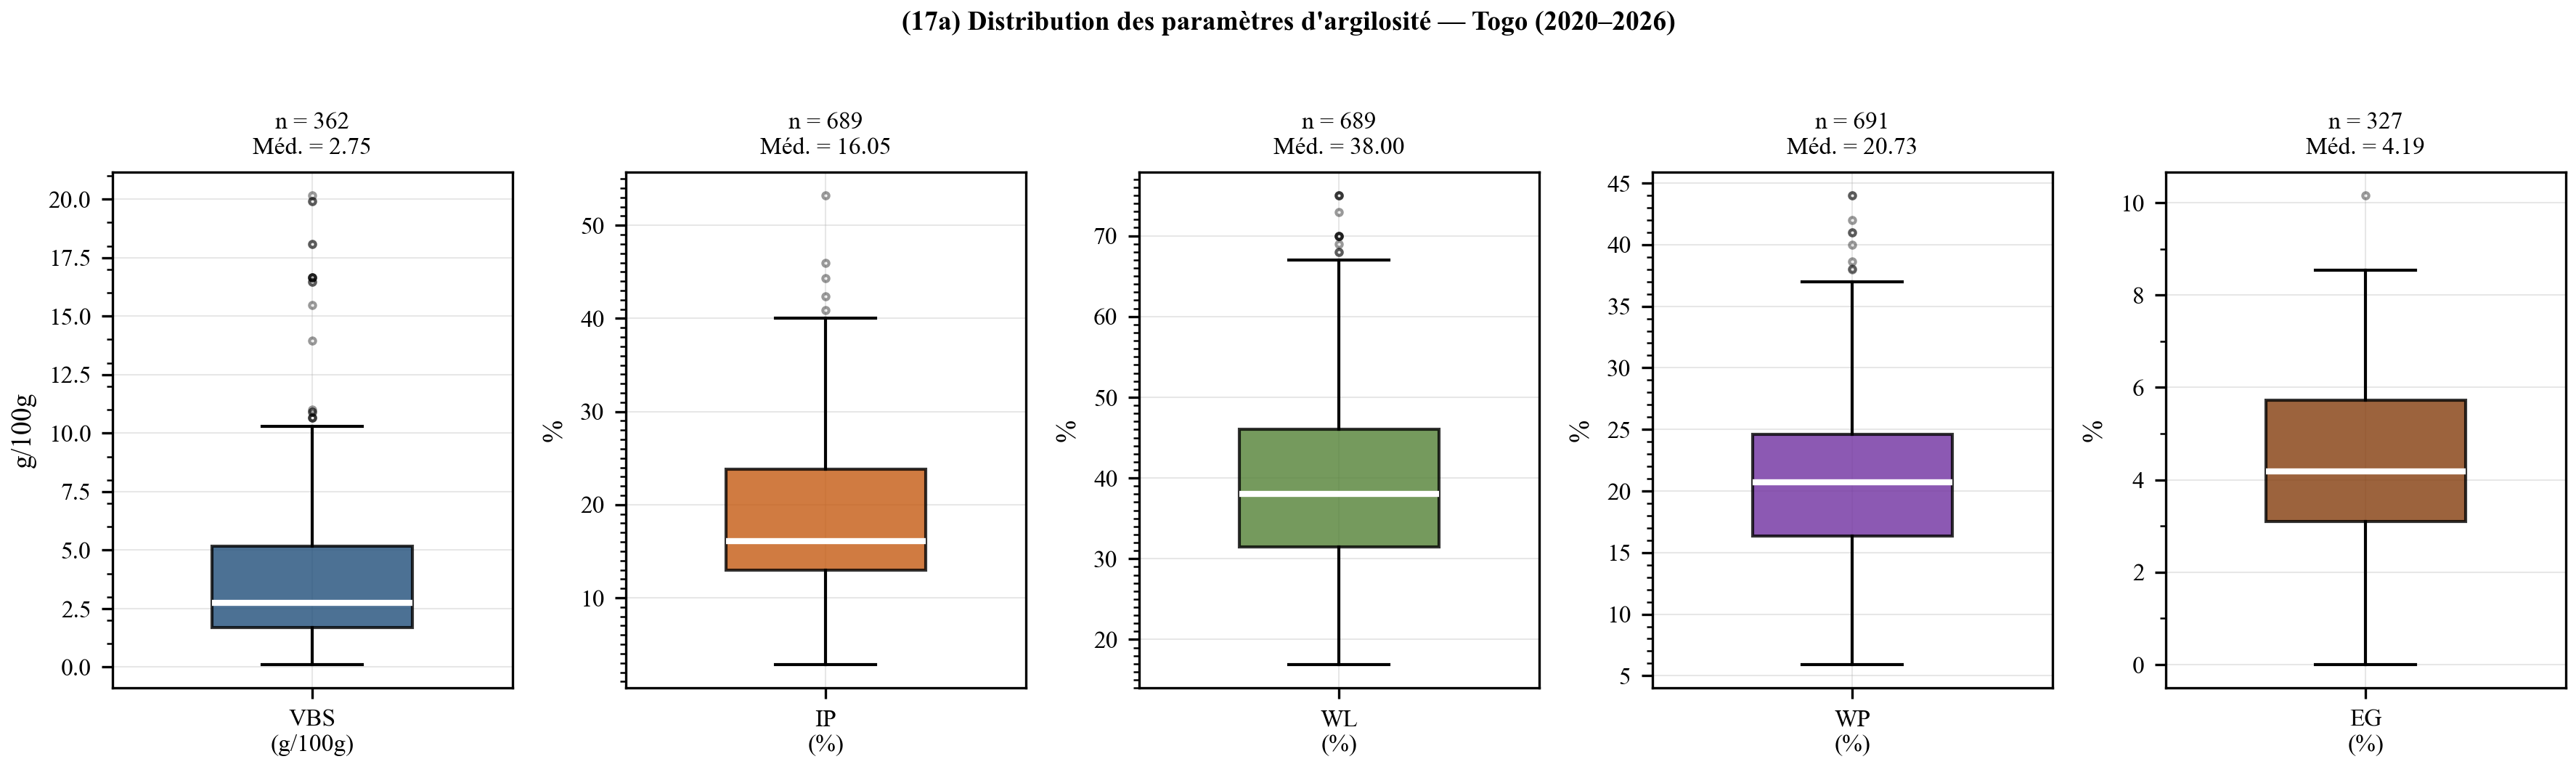
\includegraphics[width=0.97\linewidth]{figures/fig17a_argilosite_boxplots.png}
  \caption{Distribution des cinq paramètres d'argilosité/plasticité
    (mesures in situ, H1--H3 confondus, $n$ = effectif par paramètre).}
  \label{fig:boxplots}
\end{figure}

\begin{figure}[htbp]
  \centering
  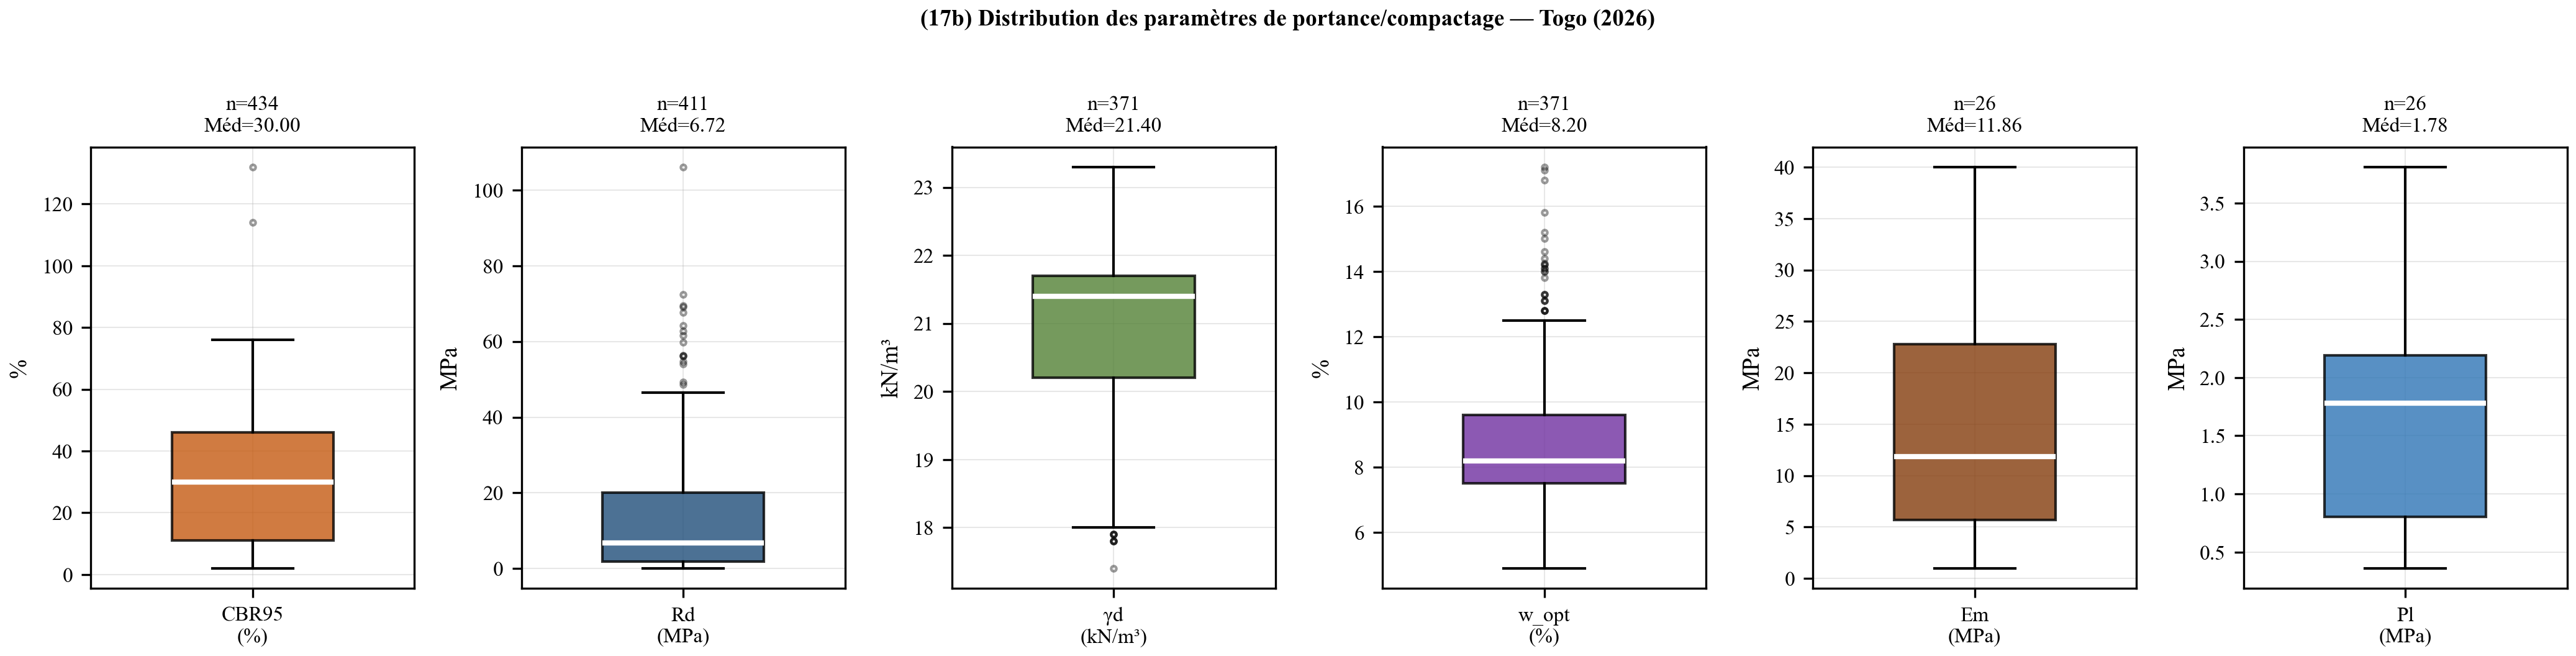
\includegraphics[width=0.97\linewidth]{figures/fig17b_portance_boxplots.png}
  \caption{Distribution des six paramètres de portance et de caractérisation
    in-situ : résistance dynamique Rd, CBR\,95\% Proctor, densité sèche
    optimale $\gamma_d$, teneur en eau optimale $w_{\mathrm{opt}}$,
    module $E_m$ et pression limite $P_l$ pressiométriques.}
  \label{fig:boxplots_portance}
\end{figure}

\subsubsection{Couches géologiques et pédologiques auxiliaires}

Cinq couches spatiales à couverture nationale (98{,}6--100\%) constituent
la base des covariables géologiques :
(1)~unités géologiques (120 polygones, 15 formations) ;
(2)~unités pédologiques (61 polygones, 13 types) ;
(3)~risque de gonflement RGA \cite{chassagneux1996} (342 entités, 5 niveaux) ;
(4)~hydrogéologie (14 polygones) ;
(5)~zones géomorphologiques spéciales (5 zones).
La combinaison de ces couches définit 79~contextes géologiques distincts.

\subsection{Covariables SCORPAN}
\label{sec:covariables}

\subsubsection{Dérivés topographiques (DSM SRTM 30~m)}

Quatre dérivés calculés sur la grille nationale à 2~km :
pente $\alpha$ (lessivage mécanique), TPI à 5~km (accumulation argileuse),
HAND (saturation hydrique, facteur critique pour EG et CBR),
et altitude DSM (latérisation).

\subsubsection{Covariables climatiques (WorldClim v2.1)}

Précipitation annuelle $P_{\mathrm{ann}}$ (BIO12), trimestre le plus sec
$P_{\mathrm{sèche}}$, et saisonnalité $\sigma_P$ (BIO15).
Les sols à forte saisonnalité développent des fentes de retrait (IP, WL élevés)
et des cycles de retrait-gonflement (EG élevé).

\subsubsection{Covariables géologiques et pédologiques}

Variables catégorielles encodées par contraste avec la moyenne nationale :
$\mathrm{enc}(c) = (\bar{z}_c - \bar{z}_{\mathrm{nat}})/\sigma_{\mathrm{nat}}$.

Le tableau~\ref{tab:covariables} récapitule les 12~covariables.

\begin{table}[htbp]
\centering\small
\caption{Covariables SCORPAN. Cat. : $S$~sol, $C$~climat, $R$~relief,
  $P$~parental, $N$~position.}
\label{tab:covariables}
\setlength{\tabcolsep}{4pt}
\begin{tabular}{@{}l@{\,}l@{\,}c@{\,}l@{}}
\toprule
Variable & Source & Cat. & Pertinence \\
\midrule
Altitude DSM        & SRTM 30m   & R & Latérisation \\
Pente $\alpha$      & SRTM dérivé& R & Lessivage mécanique \\
TPI (5~km)         & SRTM dérivé& R & Accumulation argile \\
HAND                & SRTM dérivé& R & Saturation hydrique \\
$P_{\mathrm{ann}}$  & WorldClim  & C & Altération chimique \\
$P_{\mathrm{sèche}}$& WorldClim  & C & Retrait-gonflement \\
$\sigma_P$          & WorldClim  & C & Plasticité saisonnière \\
Géologie (enc.)     & BRGM 2019  & P & Minéralogie héritée \\
Pédologie (enc.)    & FAO        & S & Type d'argile \\
Risque RGA (enc.)   & Chassagneux& S & Activité gonflante \\
Coord. Est (UTM)    & —          & N & Gradient W-E \\
Coord. Nord (UTM)   & —          & N & Gradient S-N \\
\bottomrule
\end{tabular}
\end{table}

\subsection{Formulations mathématiques des modèles}
\label{sec:modeles}

Soit $Z(\bs)$ le champ aléatoire d'un paramètre géotechnique.
L'objectif est de prédire $Z(\bs_0)$ avec incertitude $\sigma^2(\bs_0)$
sur la grille nationale ($N_g = 29\,407$ mailles).

\subsubsection{L1 — KED Hiérarchique (KED-H)}
\label{subsec:ked}

Le KED-H décompose $Z(\bs) = \mu_h(\bs) + R(\bs)$ où le résidu $R(\bs)$
est stationnaire de moyenne nulle. La dérive hiérarchique à cinq niveaux :
\begin{equation}
  \mu_h(\bs) = \begin{cases}
    \bar{z}_{\mathrm{zone}} & n_k \geq 5 \text{ (zone géomorphologique)} \\
    \bar{z}_{\mathrm{ped}}  & n_k \geq 5 \text{ (type pédologique)} \\
    \bar{z}_{\mathrm{RGA}}  & n_k \geq 5 \text{ (classe RGA)} \\
    \bar{z}_{\mathrm{géol}} & n_k \geq 5 \text{ (formation géologique)} \\
    \bar{z}_{\mathrm{nat}}  & \text{repli ultime (moyenne nationale)}
  \end{cases}
  \label{eq:prior_hierarchique}
\end{equation}
encode 79~contextes géologiques. Les Vertisols reçoivent automatiquement
$\bar{z}_{\mathrm{VBS}} \approx 8{,}7$~g/100g vs 4{,}1 en moyenne nationale.

L'estimateur $Z^*_{\KED}(\bs_0) = \sum_i \lambda_i(\bs_0)\, z(\bs_i)$
est solution du système :
\begin{equation}
  \begin{pmatrix} \bK & \mathbf{F} \\ \mathbf{F}^T & \mathbf{0} \end{pmatrix}
  \begin{pmatrix} \blambda \\ \bm{\mu} \end{pmatrix} =
  \begin{pmatrix} \mathbf{k}_0 \\ \mathbf{f}_0 \end{pmatrix}
  \label{eq:ked_system}
\end{equation}
avec variance $\sigma^2_{\KED}(\bs_0) = C(0) -
(\blambda,\bm{\mu})^T(\mathbf{k}_0,\mathbf{f}_0)^T$.

Un modèle sphérique est ajusté aux résidus empiriques :
$\gamma(h) = C_0 + C[1{,}5h/a - 0{,}5(h/a)^3]$ ($h \leq a$).
Paramètres VBS H1 : $C_0=2{,}8$, $C_0+C=14{,}0$, $a=220$~km.

\begin{figure}[htbp]
  \centering
  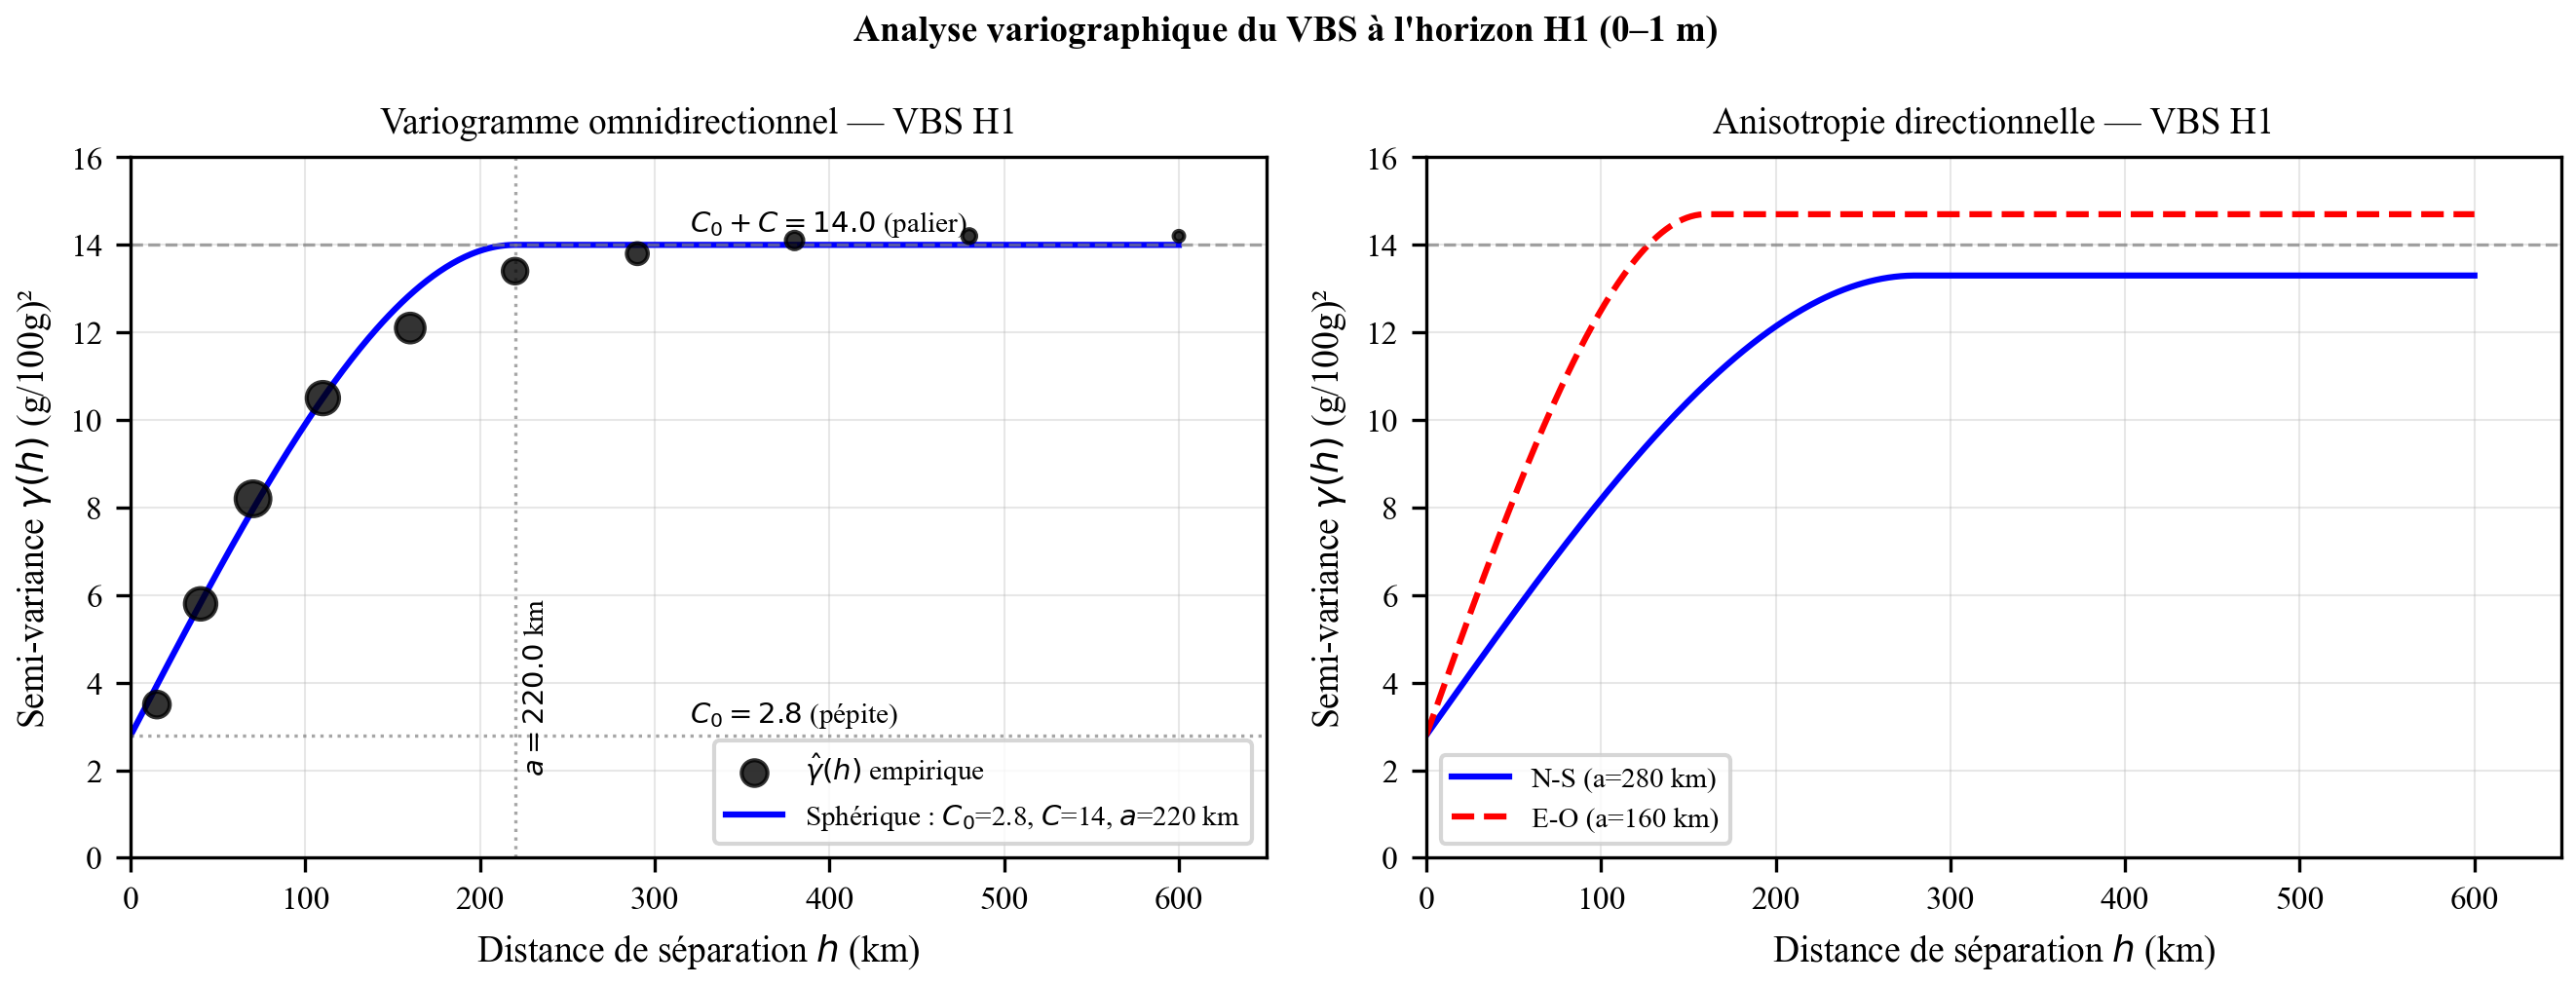
\includegraphics[width=0.97\linewidth]{figures/fig02_variogram_vbs_h1.png}
  \caption{Analyse variographique VBS H1 : modèle sphérique ajusté
    ($C_0=2{,}8$, palier 14{,}0, portée 220~km) et anisotropie N-S/E-O.}
  \label{fig:variogram}
\end{figure}

\subsubsection{L2a — RK-SCORPAN}
\label{subsec:rk}

Régression Ridge + krigeage des résidus \cite{hengl2007regression} :
\begin{equation}
  \hat{\bm{\beta}} = (\mathbf{X}^T\mathbf{X} + \lambda_R \mathbf{I})^{-1}\mathbf{X}^T\mathbf{z}
  \label{eq:rk}
\end{equation}
$\lambda_R^* = 0{,}18$ (calibré par LOO-CV, VBS H1, figure~\ref{fig:ridge_cv}).
Le LOO-CV RK est \emph{complet} : ré-estimation Ridge \emph{et} krigeage des
résidus à chaque itération (évite une sous-estimation de 15--30\%
de l'erreur réelle).

\subsubsection{L2b — Fusion Bayésienne BLUP}
\label{subsec:fusion}

Combinaison BLUP pondérée \cite{chilesdelfiner2012}, $w_j = 1/\sigma^2_j(\bs_0)$ :
\begin{equation}
  Z^*_{\BLUP} =
    \frac{w_{\KED} Z^*_{\KED} + w_{\RK} Z^*_{\RK}}{w_{\KED}+w_{\RK}}
  \label{eq:blup}
\end{equation}
\begin{equation}
  \sigma^2_{\BLUP} = \frac{\sigma^2_{\KED}\sigma^2_{\RK}}
    {\sigma^2_{\KED}+\sigma^2_{\RK}}
    < \min\!\bigl(\sigma^2_{\KED},\sigma^2_{\RK}\bigr)
  \label{eq:blup_var}
\end{equation}
Propriété garantie mathématiquement dans 100\% des mailles.
Aucune variance proxy utilisée : $\sigma^2_j$ provient directement du
krigeage ordinaire des résidus.

\subsubsection{L3 — VfS-PLS (Sentinel-2)}
\label{subsec:vfs}

Régression PLS sur indices spectraux SWIR de Sentinel-2
($I_{\mathrm{argile}}=B_{11}/B_{12}$, $I_{\mathrm{SWIR}}$, NDVI, $I_{\mathrm{Fe}}$,
composite médian 2023--2024) \cite{viscarra2006data}.
$q=3$ composantes optimisées par LOO-CV.
Variance homoscédastique : $\hat{\sigma}^2_{\mathrm{VfS}} = \mathrm{RMSE}_{LOO}^2$.

\subsubsection{L4 — MTGP/ICM}
\label{subsec:mtgp}

Modèle de Coregionalisation Intrinsèque (ICM, rang $r=2$)
\cite{journelhijbregts1978} :
$Z_d(\bs) = \sum_l a_{dl} G_l(\bs) + \varepsilon_d(\bs)$,
covariance conjointe :
$\mathrm{Cov}[Z_d(\bs),Z_{d'}(\bs')] = \sum_l a_{dl}a_{d'l} k_l(\bs,\bs')$
où $k_l$ est le noyau RBF. Implémentation GPflow (SwitchedLikelihood,
format Y$=[$ valeur, output\_index $]$, optimiseur Adam, 500 itérations).
Le tableau~\ref{tab:correlations} justifie l'utilisation du MTGP.

\begin{table}[htbp]
\centering\small
\caption{Corrélations de Pearson des paramètres d'argilosité
  (mesures in situ, horizons confondus, base de données 2026).
  \textbf{Gras} : $|r| > 0{,}7$.}
\label{tab:correlations}
\begin{tabular}{lccccc}
\toprule
 & VBS & IP & WL & WP & EG \\
\midrule
VBS & 1,000 & 0,319 & 0,254 & $-$0,024 & 0,363 \\
IP  & 0,319 & 1,000 & \textbf{0,773} & $-$0,062 & \textbf{0,721} \\
WL  & 0,254 & \textbf{0,773} & 1,000 & 0,586 & \textbf{0,671} \\
WP  & $-$0,024 & $-$0,062 & 0,586 & 1,000 & 0,143 \\
EG  & 0,363 & \textbf{0,721} & \textbf{0,671} & 0,143 & 1,000 \\
\bottomrule
\end{tabular}
\end{table}

\begin{figure}[htbp]
  \centering
  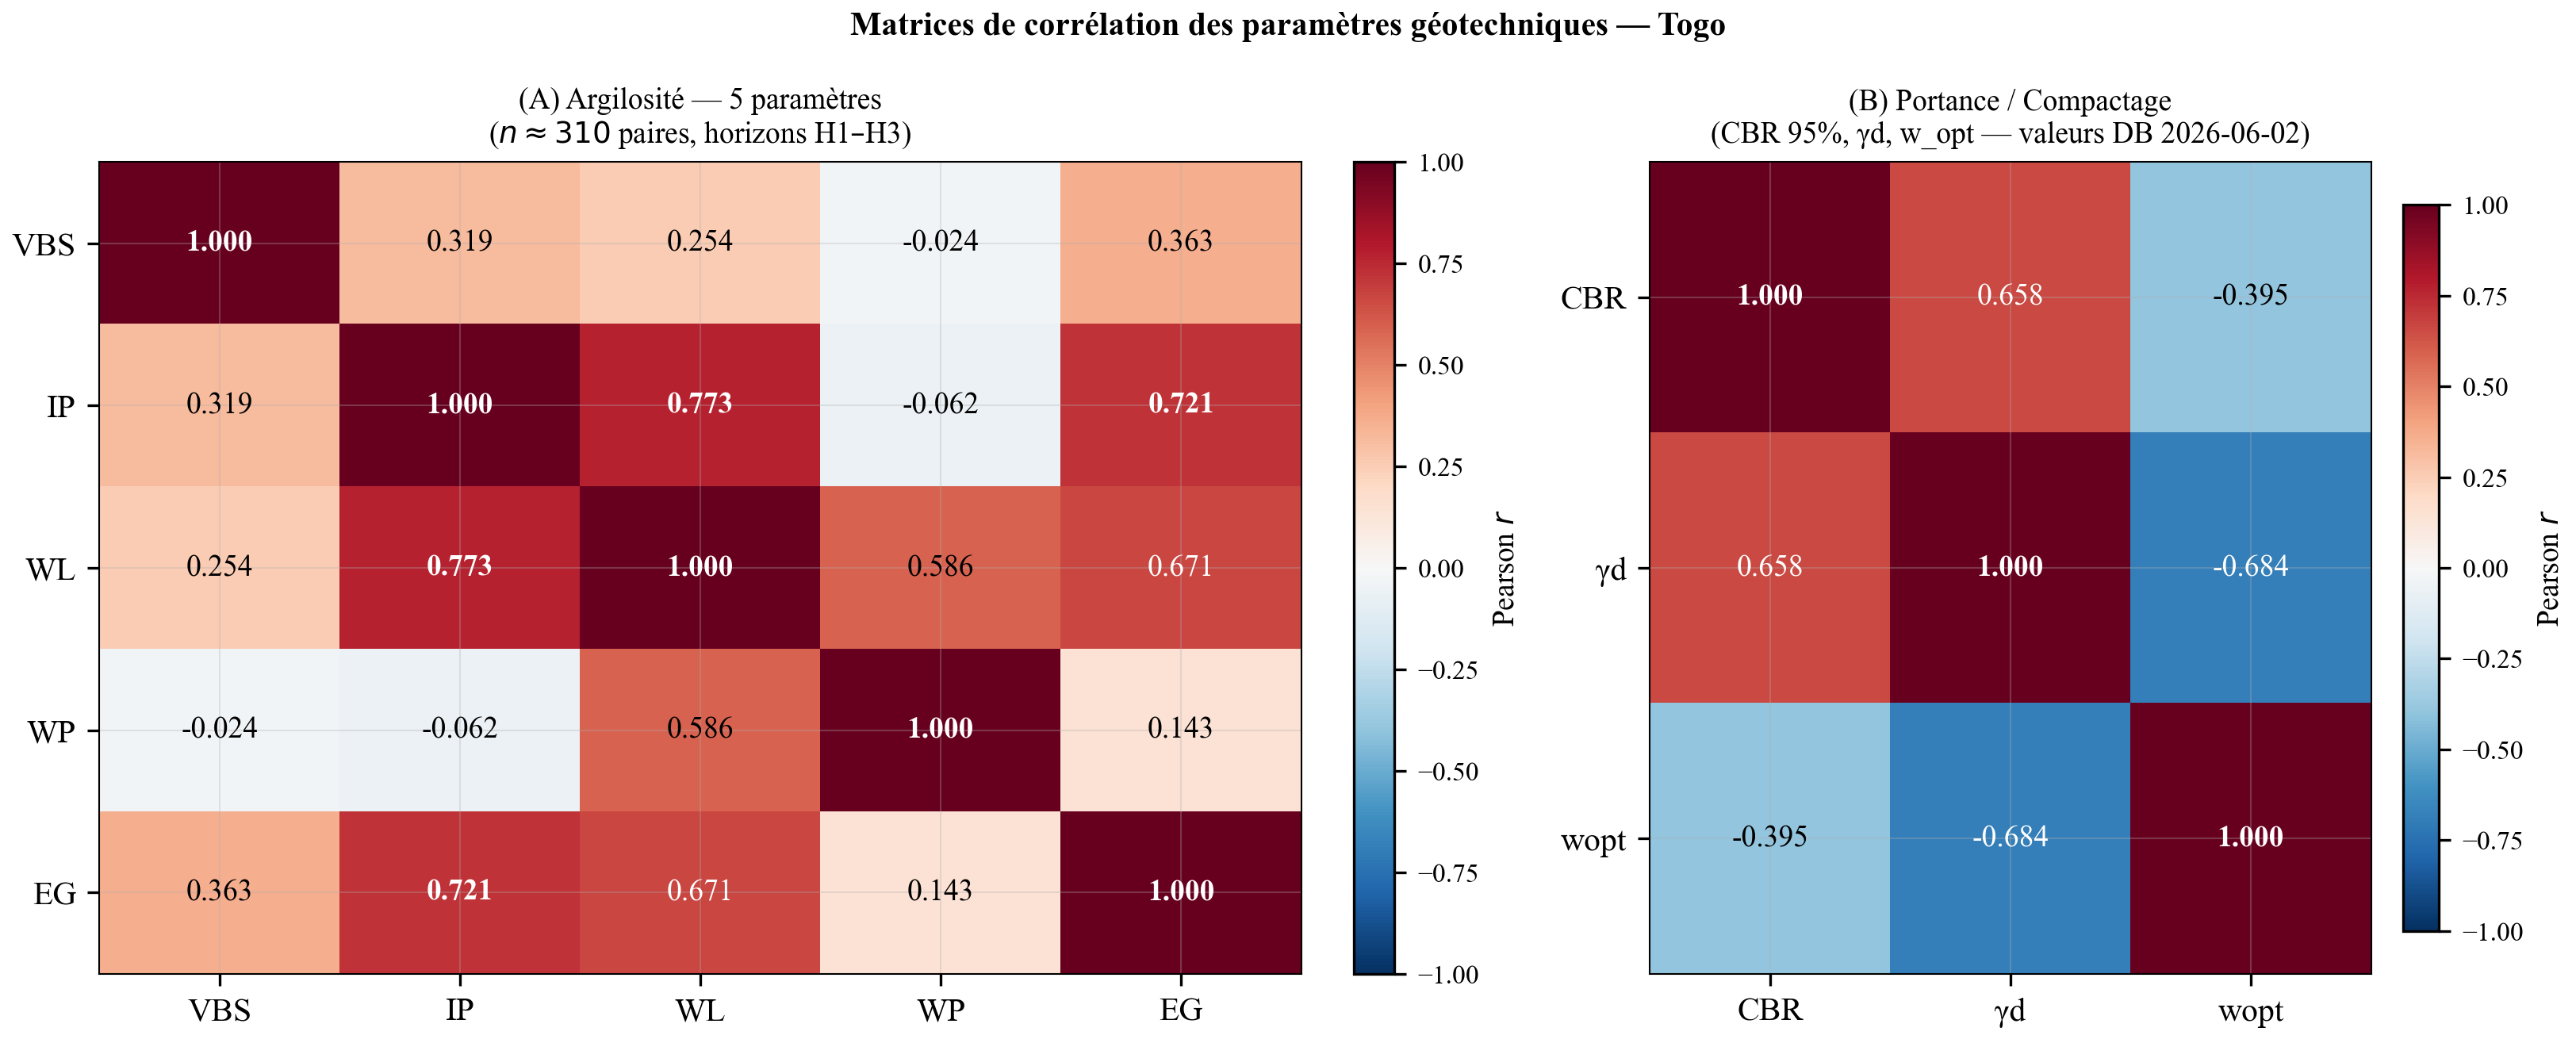
\includegraphics[width=0.97\linewidth]{figures/fig04_correlation_matrix.png}
  \caption{Matrices de corrélation de Pearson calculées sur la base de
    données (2026). \textit{Panneau A (gauche) :} cinq paramètres
    d'argilosité --- les corrélations IP-WL ($r=0{,}773$) et IP-EG
    ($r=0{,}721$) justifient la modélisation conjointe par MTGP/ICM.
    \textit{Panneau B (droite) :} trois paramètres de portance Proctor ---
    la forte corrélation négative $\gamma_d$-$w_{\mathrm{opt}}$
    ($r=-0{,}684$) reflète la courbe Proctor.}
  \label{fig:correlations}
\end{figure}

\subsection{Implémentation et validation croisée}
\label{sec:pipeline}

Le pipeline comprend cinq niveaux : import terrain → covariables SCORPAN →
modèles L1--L4 → fusion bayésienne → stockage des 441\,105 prédictions.
La figure~\ref{fig:pipeline} décrit l'architecture.

\begin{figure}[htbp]
  \centering
  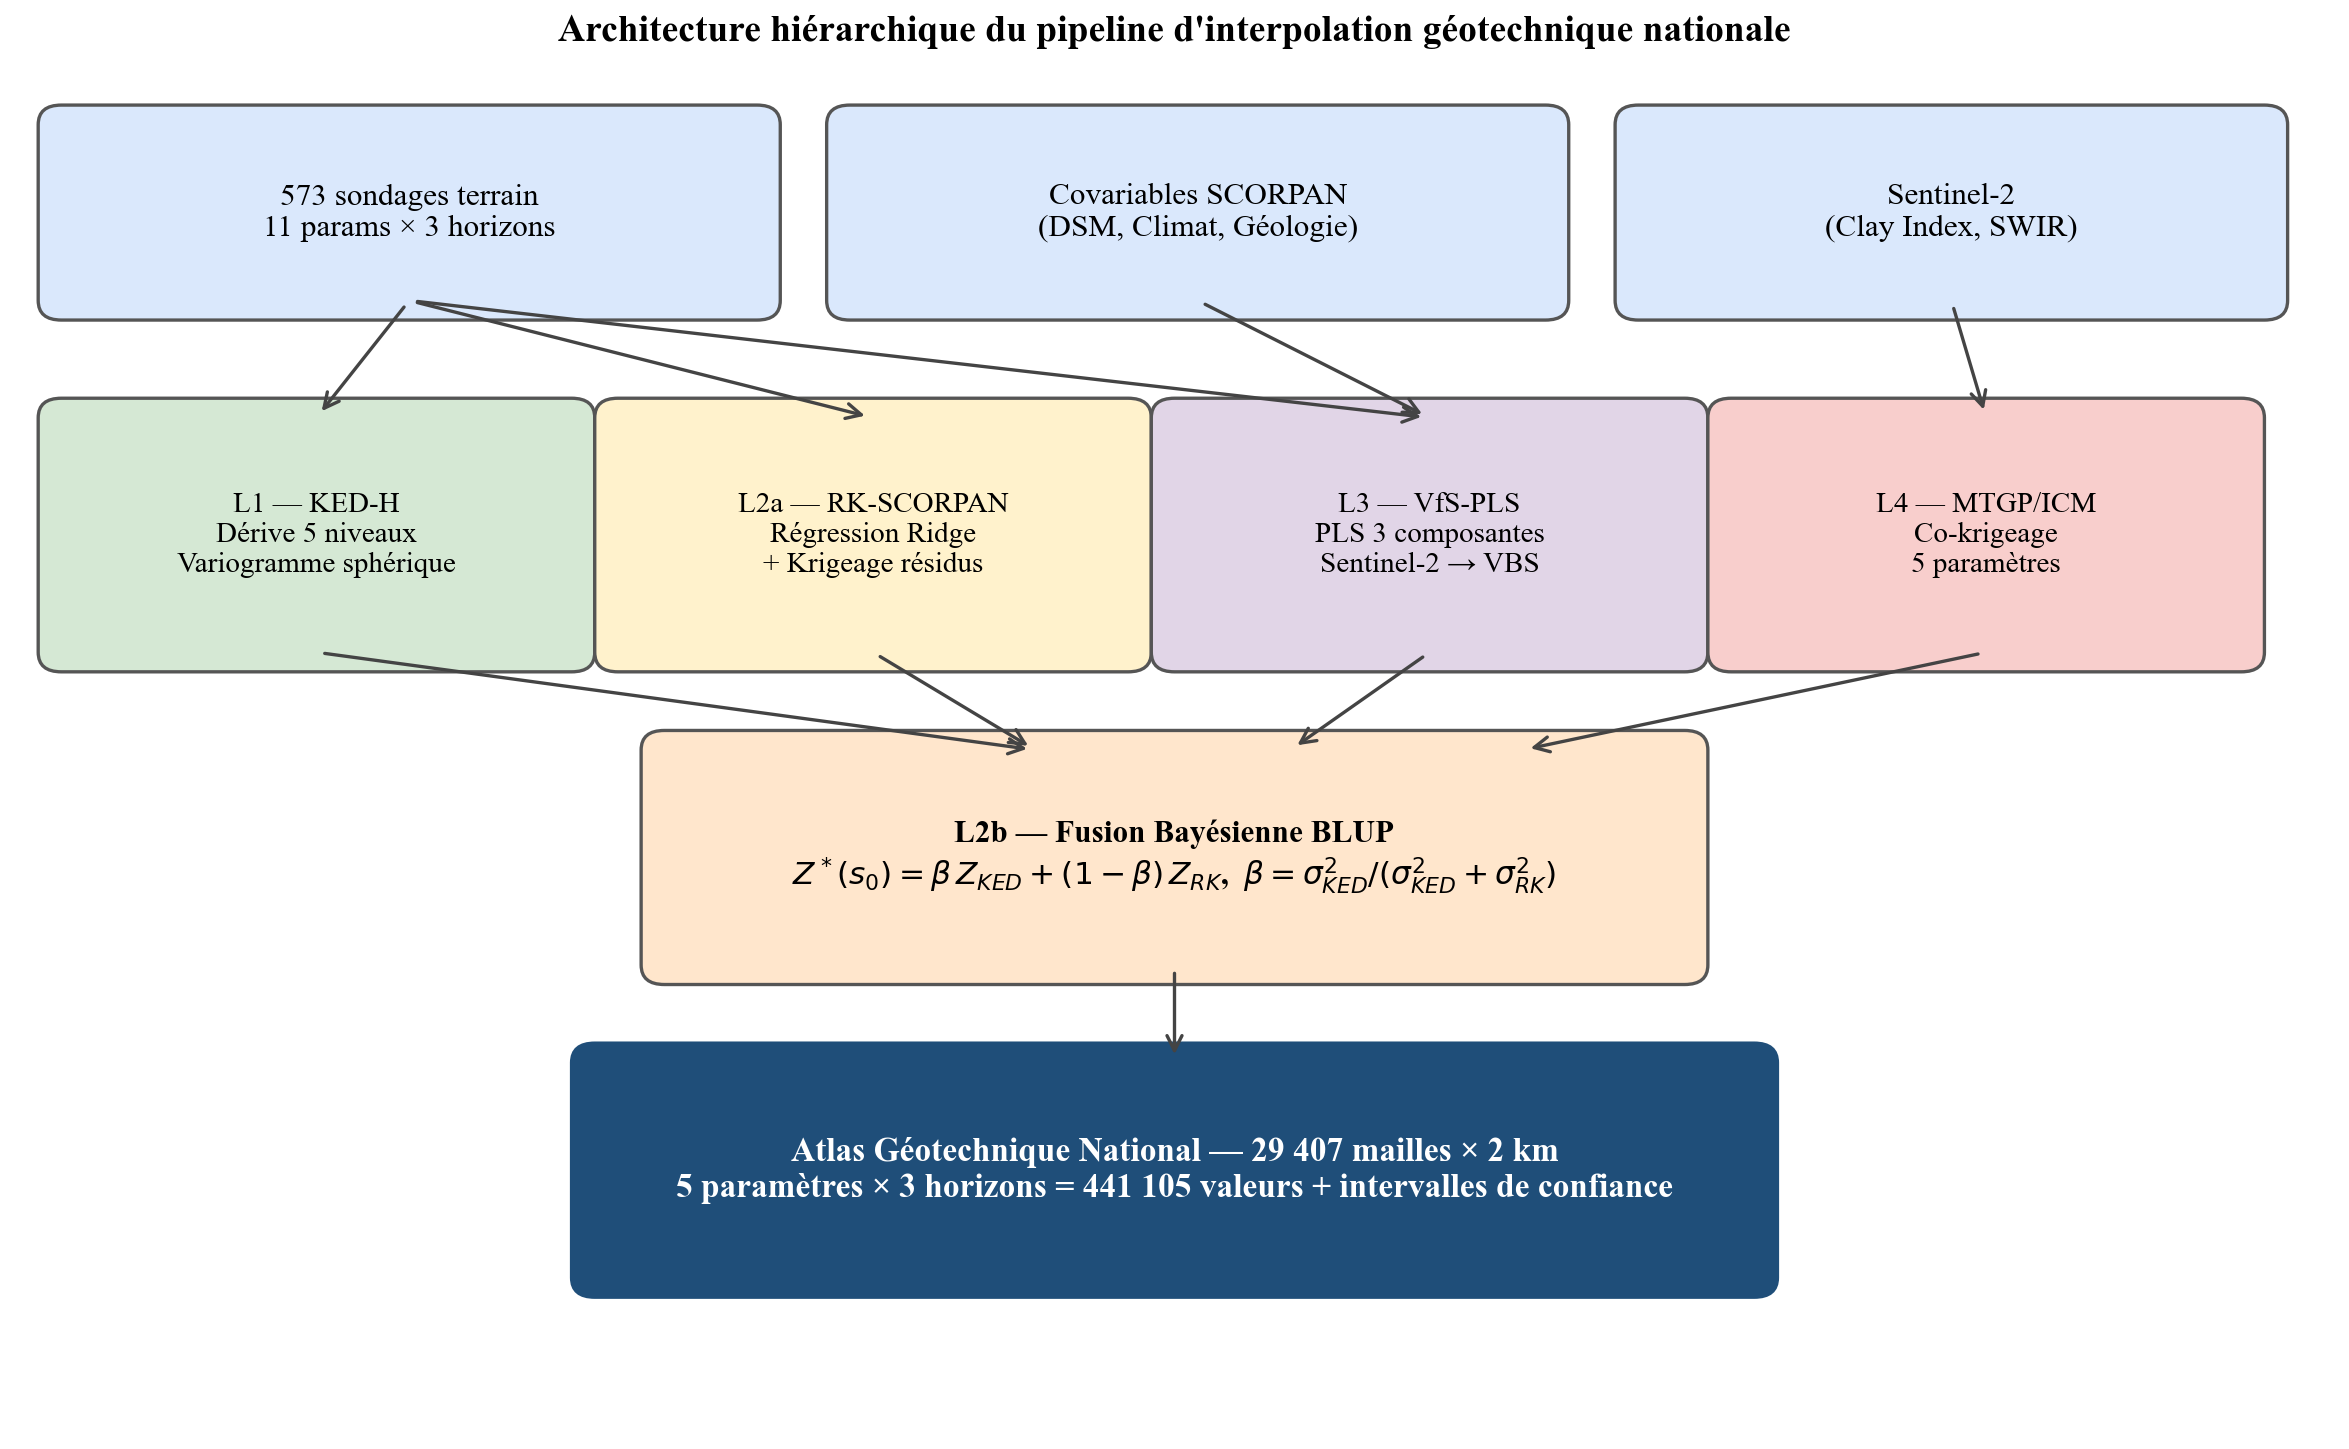
\includegraphics[width=0.97\linewidth]{figures/fig08_pipeline_schema.png}
  \caption{Architecture hiérarchique du pipeline L1--L4.
    L1 et L2a alimentent L2b (fusion). L3 et L4 sont indépendants.
    Sortie : 29\,407 mailles × 11~paramètres × 3~horizons.}
  \label{fig:pipeline}
\end{figure}

La performance est évaluée par LOO-CV complet :
$\mathrm{RMSE}_{\mathrm{LOO}} = \sqrt{\frac{1}{n}\sum_i [z(\bs_i)-Z^*_{(-i)}(\bs_i)]^2}$.

\begin{figure}[htbp]
  \centering
  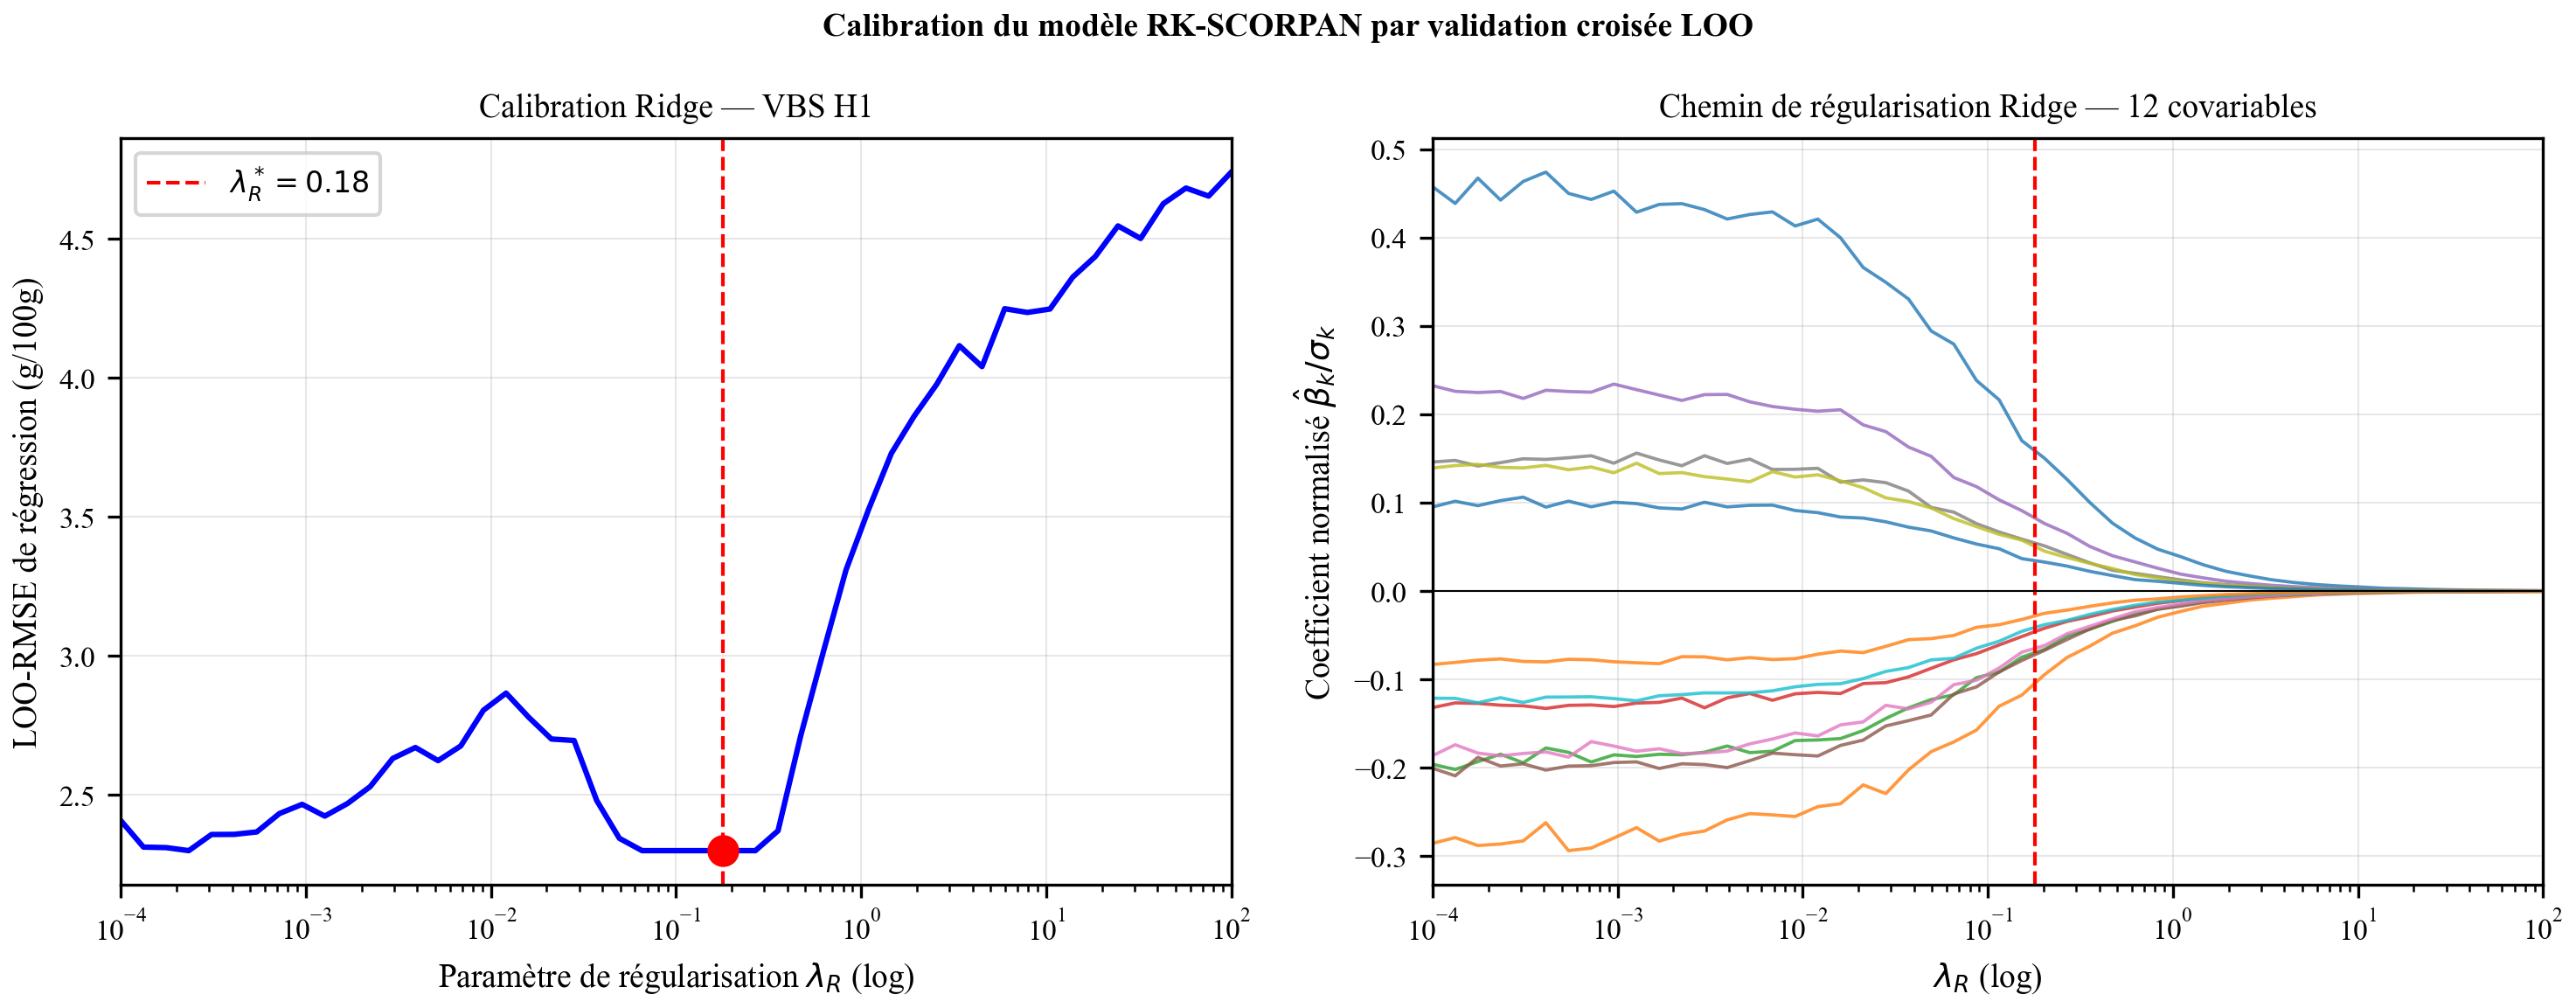
\includegraphics[width=0.97\linewidth]{figures/fig11_ridge_calibration.png}
  \caption{Calibration Ridge par LOO-CV (VBS H1) : courbe RMSE-$\lambda_R$
    et chemins de régularisation des 12~covariables ($\lambda_R^*=0{,}18$).}
  \label{fig:ridge_cv}
\end{figure}

% ══════════════════════════════════════════════════════════════════════════════
\section{Résultats}
\label{sec:resultats}
% ══════════════════════════════════════════════════════════════════════════════

\subsection{Performance LOO-CV — Comparaison inter-modèles}
\label{subsec:loo_resultats}

\subsubsection{Vue d'ensemble : tous paramètres H1}

La figure~\ref{fig:loo_rmse} présente les LOO-RMSE KED-H pour l'ensemble
des 11~paramètres à l'horizon H1, et compare KED-H vs RK-SCORPAN pour les
cinq paramètres d'argilosité. Sur 15~comparaisons directes (H1/H2/H3 × 5
paramètres), KED-H domine sur 6~critères (IP-H1/H3, WL-H1/H2/H3, WP-H2)
et RK sur 9. Le tableau~\ref{tab:loo_rmse} présente les valeurs H1.

\begin{figure}[htbp]
  \centering
  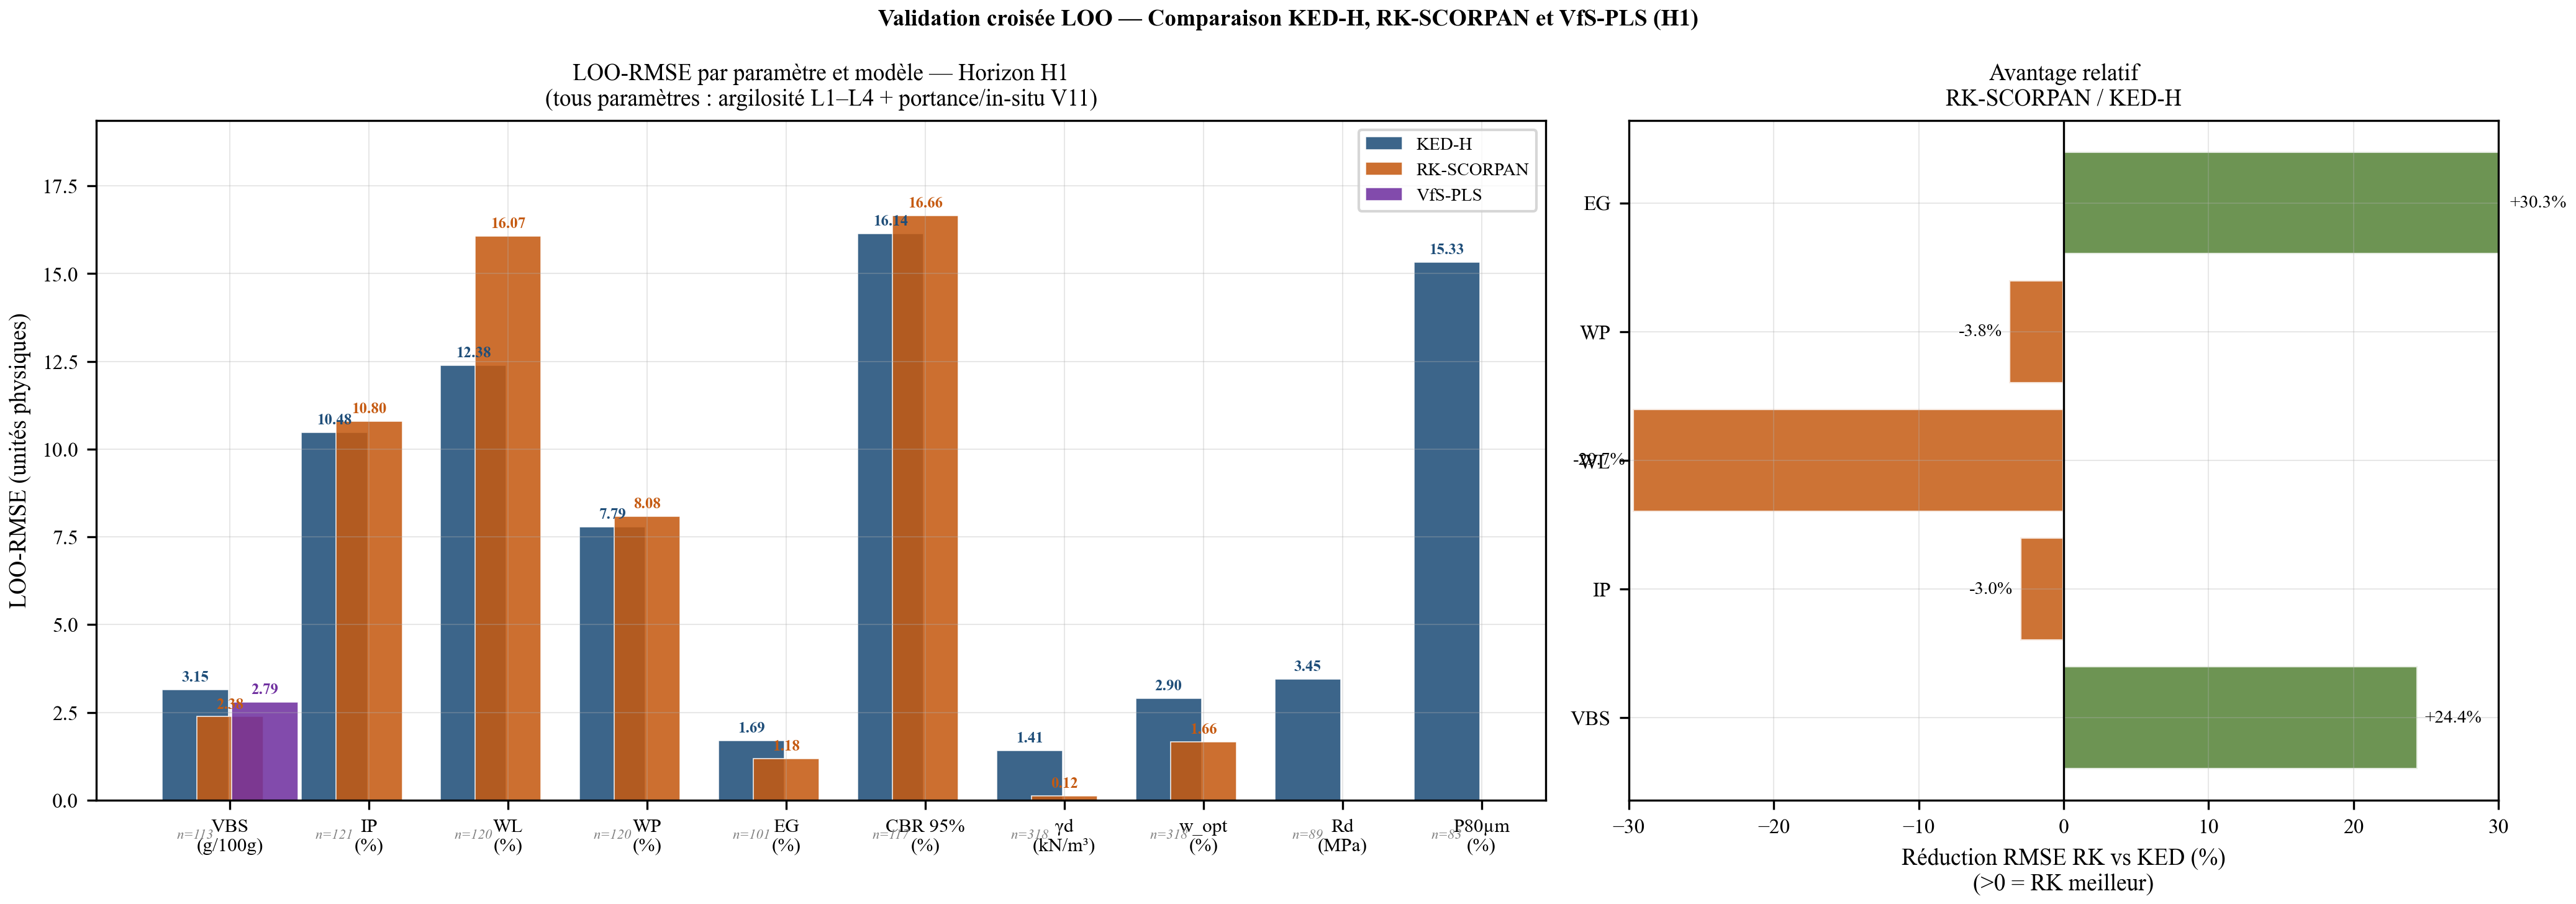
\includegraphics[width=0.97\linewidth]{figures/fig03_loo_rmse_comparison.png}
  \caption{\textit{Gauche (panneau A) :} LOO-RMSE KED-H H1 pour tous les
    paramètres (argilosité en bleu, portance en rouge). Taille n indiquée.
    \textit{Droite (panneau B) :} réduction relative RK vs KED pour les
    paramètres d'argilosité ($>0$ = RK meilleur).}
  \label{fig:loo_rmse}
\end{figure}

\begin{table}[htbp]
\centering\small
\caption{LOO-RMSE H1 — paramètres d'argilosité/plasticité.
  \textbf{Gras} = meilleur modèle. Score 15~comparaisons en annexe.}
\label{tab:loo_rmse}
\begin{tabular}{lcccc}
\toprule
Param. & Unité & KED-H & RK-SCORPAN & VfS-PLS \\
\midrule
VBS  & g/100g & 3,147          & \textbf{2,625} & 2,788 \\
IP   & \%     & \textbf{10,481}& 12,509         & —     \\
WL   & \%     & \textbf{12,384}& 16,186         & —     \\
WP   & \%     & 7,788          & \textbf{5,349} & —     \\
EG   & \%     & 1,692          & \textbf{1,149} & —     \\
\midrule
Score H1 & & 2/5 & 3/5 & \\
\bottomrule
\end{tabular}
\end{table}

\subsubsection{Paramètres de portance et de caractérisation in-situ}

Le tableau~\ref{tab:loo_v11} regroupe les LOO-RMSE KED-H pour les six
paramètres de portance mécanique et les essais in-situ.
Pour ces paramètres, le modèle RK-SCORPAN n'a pas encore été calibré~: la
Régression Kriging requiert un recalcul des covariables spécifiques à la
portance (densité du réseau hydrographique, altérite, compacité des formations).

\begin{table}[htbp]
\centering\small
\caption{LOO-RMSE KED-H — paramètres de portance et in-situ, par horizon.}
\label{tab:loo_v11}
\begin{tabular}{lcrrrr}
\toprule
Paramètre & Unité & $n_{\mathrm{H1}}$ & H1 & H2 & H3 \\
\midrule
CBR 95\%   & \%    & 117 & 16,14 & —     & —     \\
$\gamma_d$ & kN/m³ & 318 & 1,41  & —     & —     \\
$w_{\mathrm{opt}}$ & \% & 318 & 2,90 & — & —  \\
Rd         & MPa   & 89  & 3,45  & 7,01  & 14,16 \\
$E_m$      & MPa   & —   & —     & —     & 13,31 \\
$P_l$      & MPa   & —   & —     & —     & 0,988 \\
\bottomrule
\multicolumn{6}{l}{\small — : $n < 10$ à cet horizon.}
\end{tabular}
\end{table}

\subsubsection{Analyse par horizon — dégradation avec la profondeur}

La figure~\ref{fig:multihorizon} présente les LOO-RMSE pour l'ensemble
des paramètres, groupés par horizon. On observe :
(1)~pour les paramètres d'argilosité, une légère dégradation H1 → H2
puis récupération à H3 (corrélation $r_{\mathrm{H1,H3}}=0{,}511$) ;
(2)~pour Rd, une forte dégradation H1→H3 ($3{,}45 \to 14{,}16$~MPa),
cohérente avec l'hétérogénéité de l'altérite en profondeur ($n_{\mathrm{H3}}=272$
mesures éparses) ; (3)~l'anomalie RK H2 pour VBS (4{,}81 vs 3{,}20 KED)
reflète la perte de corrélation entre covariables de surface et horizon 1--1{,}5~m.

\begin{figure}[htbp]
  \centering
  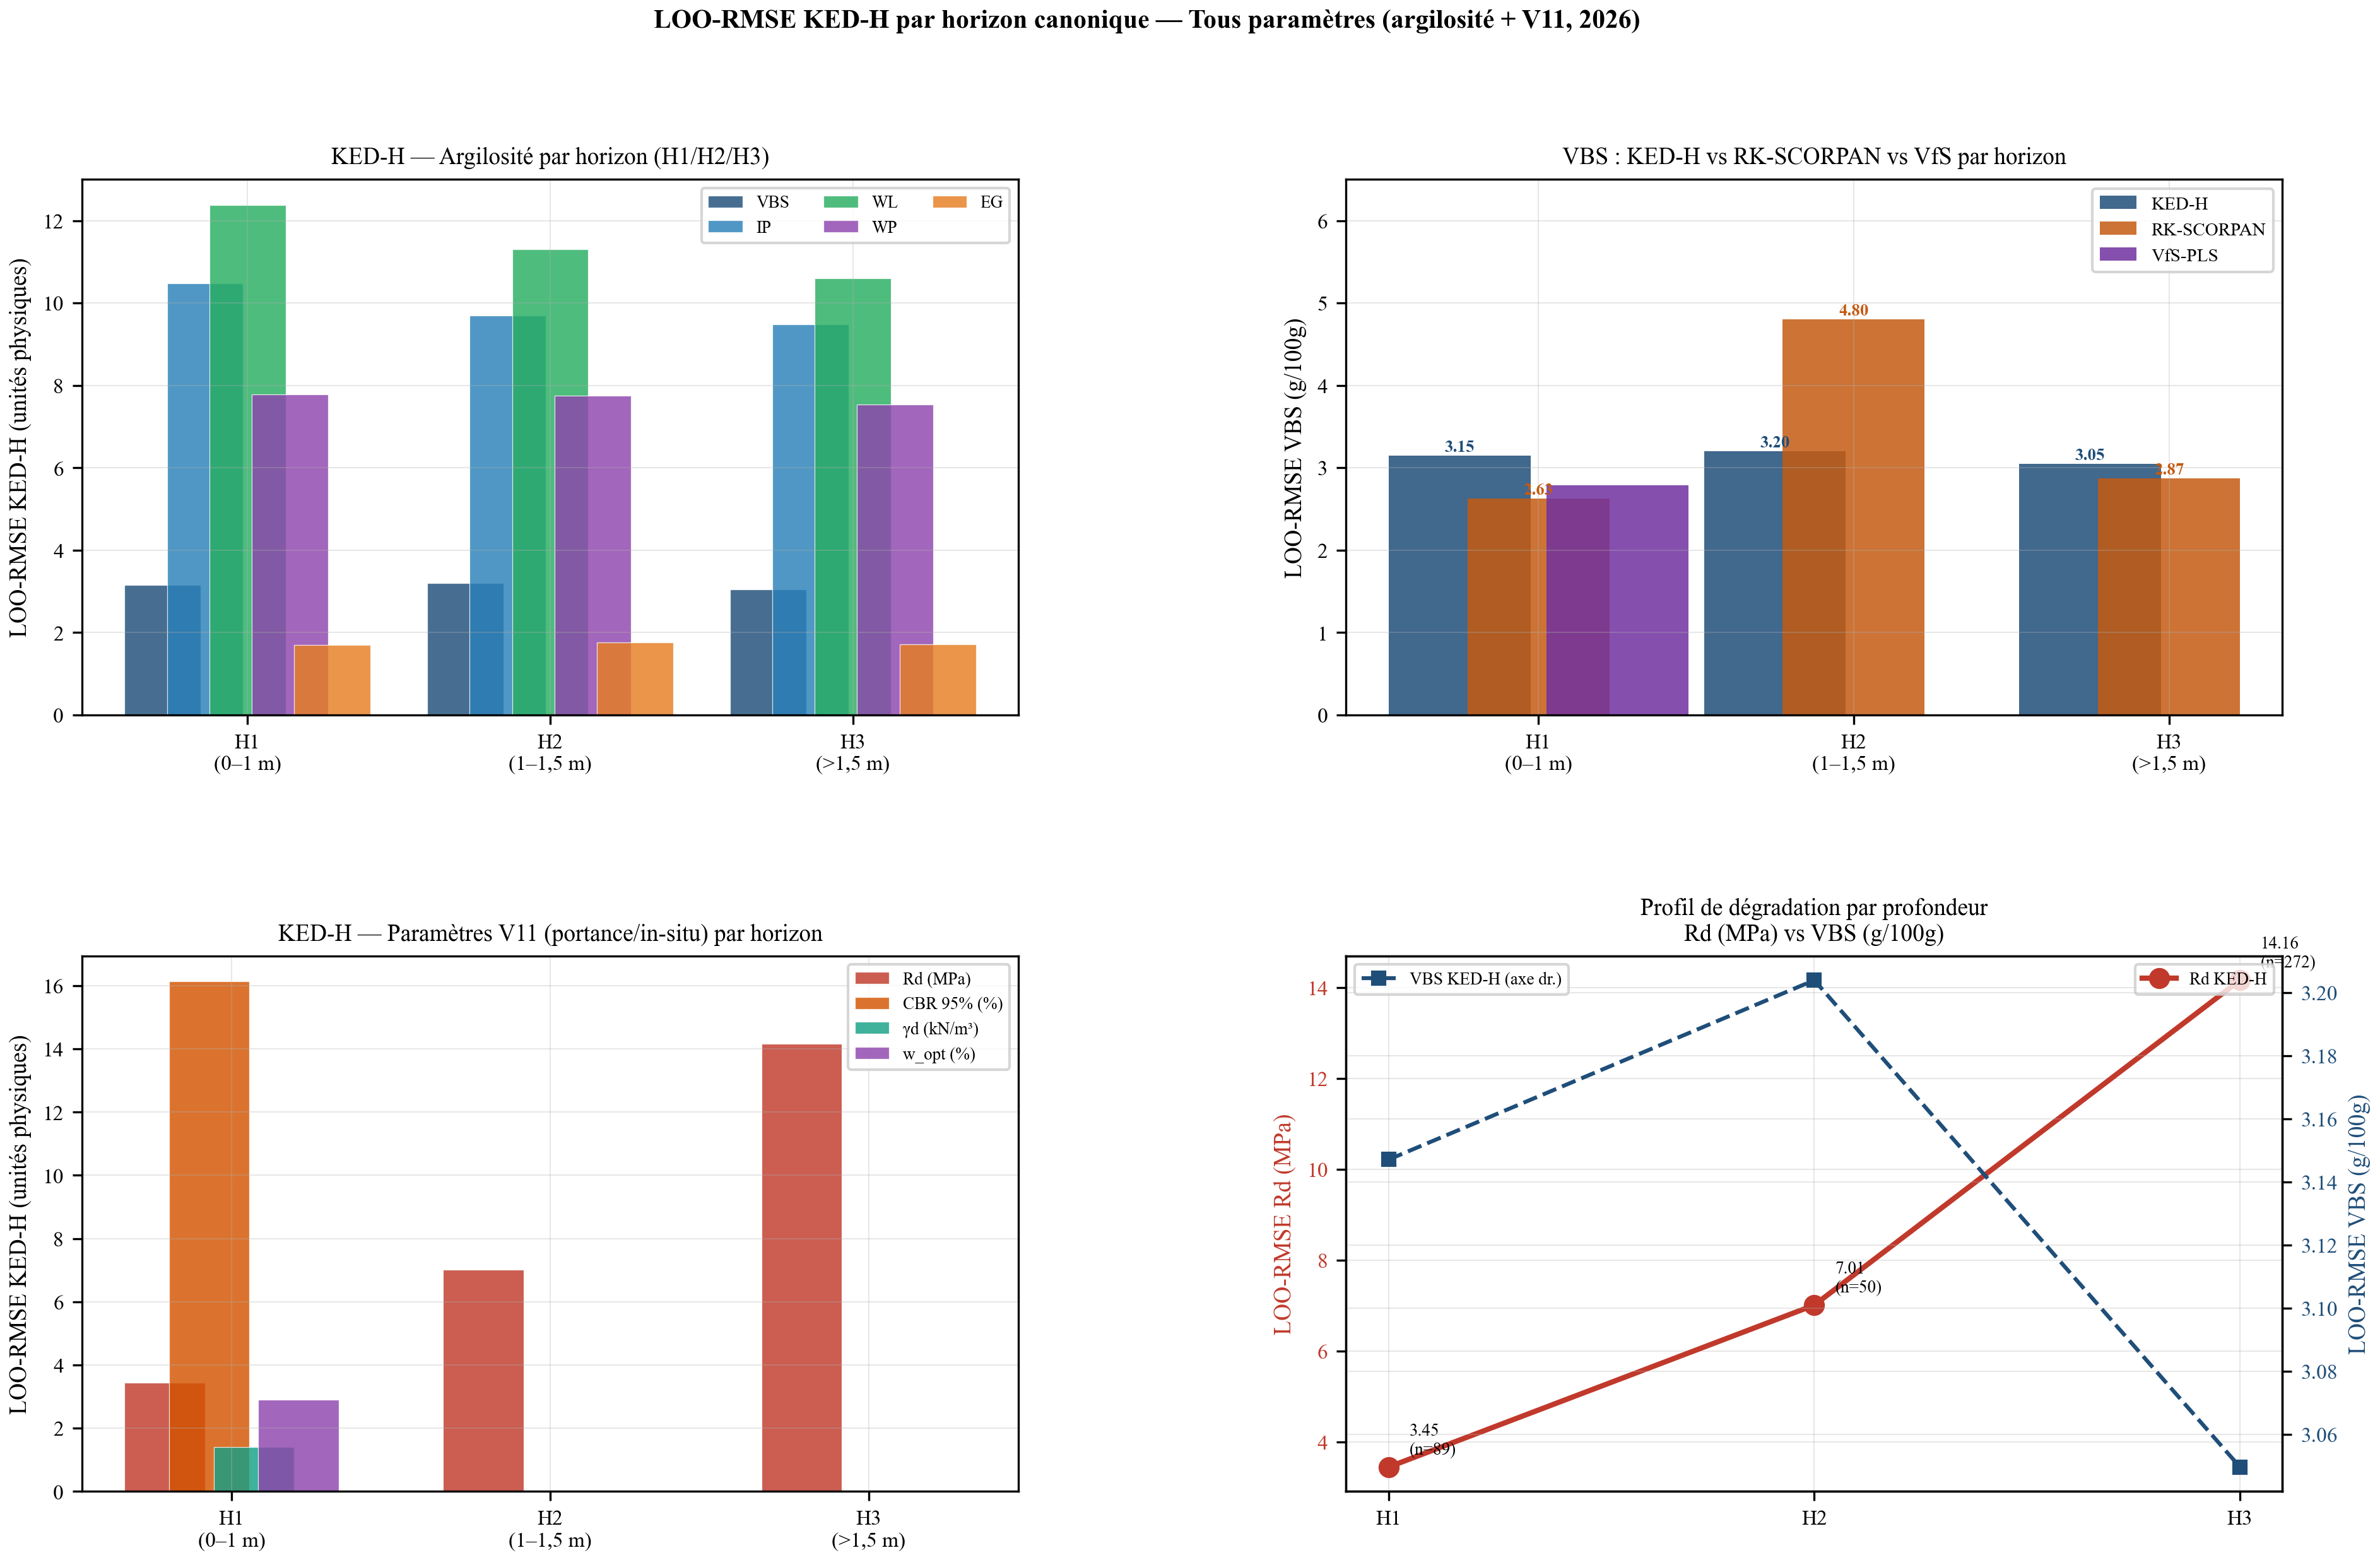
\includegraphics[width=0.97\linewidth]{figures/fig10_loo_multihorizon.png}
  \caption{LOO-RMSE par horizon H1/H2/H3 — quatre panneaux :
    (A)~KED-H paramètres d'argilosité, (B)~VBS : KED-H vs RK-SCORPAN vs VfS-PLS,
    (C)~KED-H paramètres de portance, (D)~profil de dégradation Rd (rouge, MPa)
    vs VBS (bleu, g/100g) avec la profondeur.}
  \label{fig:multihorizon}
\end{figure}

\begin{figure}[htbp]
  \centering
  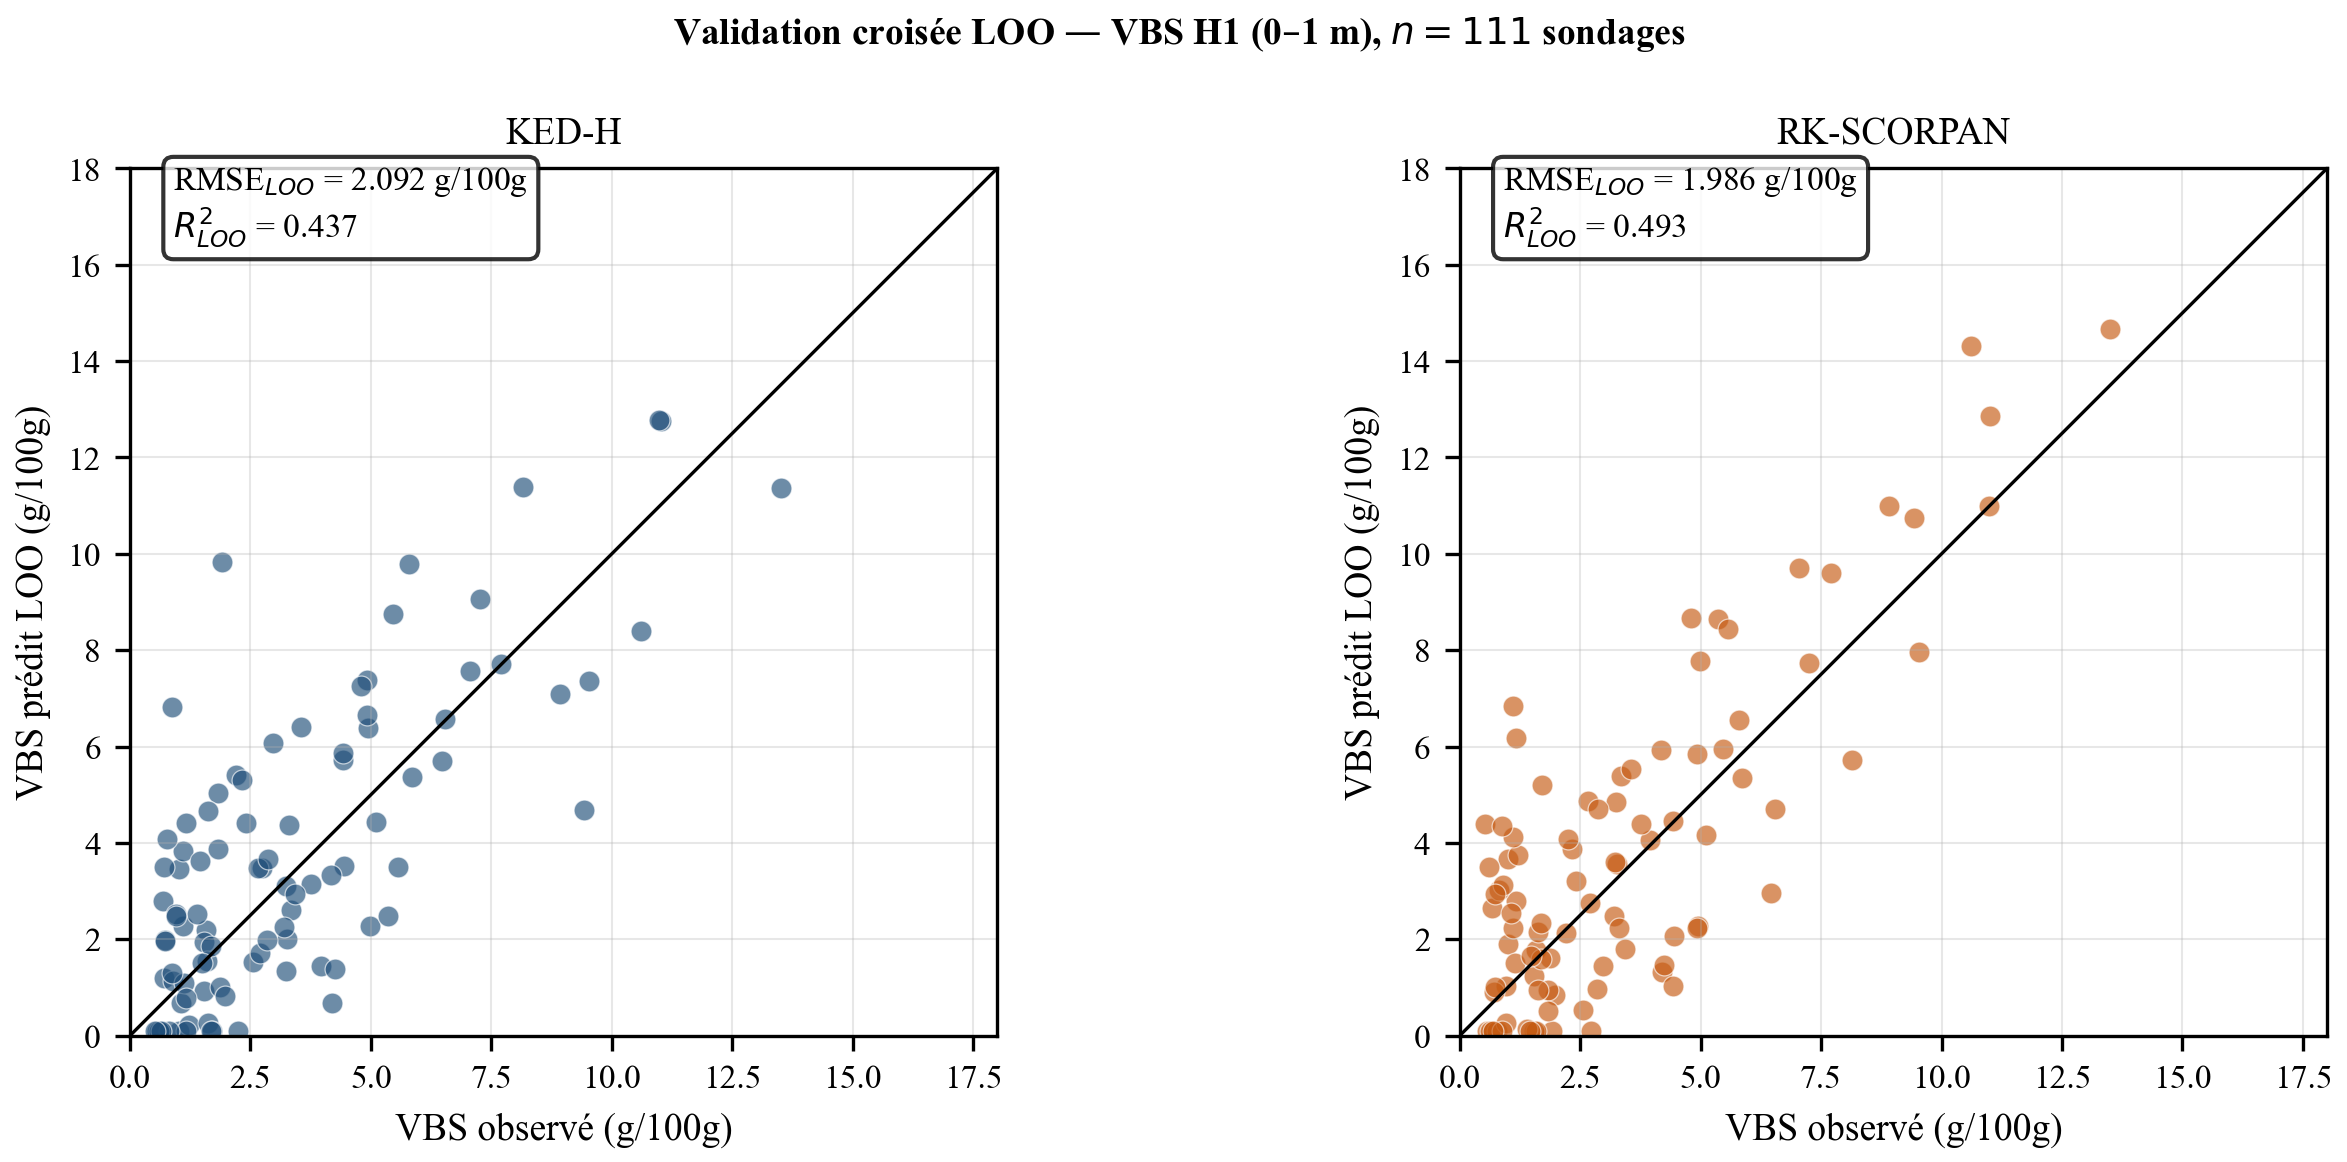
\includegraphics[width=0.97\linewidth]{figures/fig06_loo_scatter_vbs.png}
  \caption{Diagramme prédit vs observé (LOO-CV) VBS H1 ($n=113$).
    Gauche : KED-H (RMSE$=3{,}147$). Droite : RK-SCORPAN (RMSE$=2{,}625$).}
  \label{fig:loo_scatter}
\end{figure}

\subsection{Réduction de variance par Fusion Bayésienne}
\label{subsec:fusion_res}

Le tableau~\ref{tab:variance} quantifie la réduction induite par la Fusion BLUP.
La réduction moyenne de 47{,}9\% est proche du maximum théorique de 50\%
(atteint quand $\sigma^2_{\KED} = \sigma^2_{\RK}$), confirmant que les deux
modèles ont des précisions comparables mais des structures spatiales
complémentaires.

\begin{table}[htbp]
\centering\small
\caption{Variance moyenne de krigeage $\bar{\sigma}^2$ par modèle (H1).}
\label{tab:variance}
\begin{tabular}{lcccc}
\toprule
Param. & KED-H  & RK     & Fusion & Réduc. \\
\midrule
VBS    & 12,45  & 10,60  & \textbf{5,73}  & 45,9\% \\
IP     & 90,99  & 79,87  & \textbf{42,33} & 47,0\% \\
WL     & 174,15 & 140,36 & \textbf{77,63} & 44,7\% \\
WP     & 54,54  & 60,37  & \textbf{28,70} & 47,4\% \\
EG     & 2,68   & 2,55   & \textbf{1,30}  & 48,8\% \\
\midrule
\multicolumn{3}{l}{\textbf{Moyenne}} &
  \multicolumn{2}{r}{\textbf{47,9\%~±~1,5\%}} \\
\bottomrule
\end{tabular}
\end{table}

\begin{figure}[htbp]
  \centering
  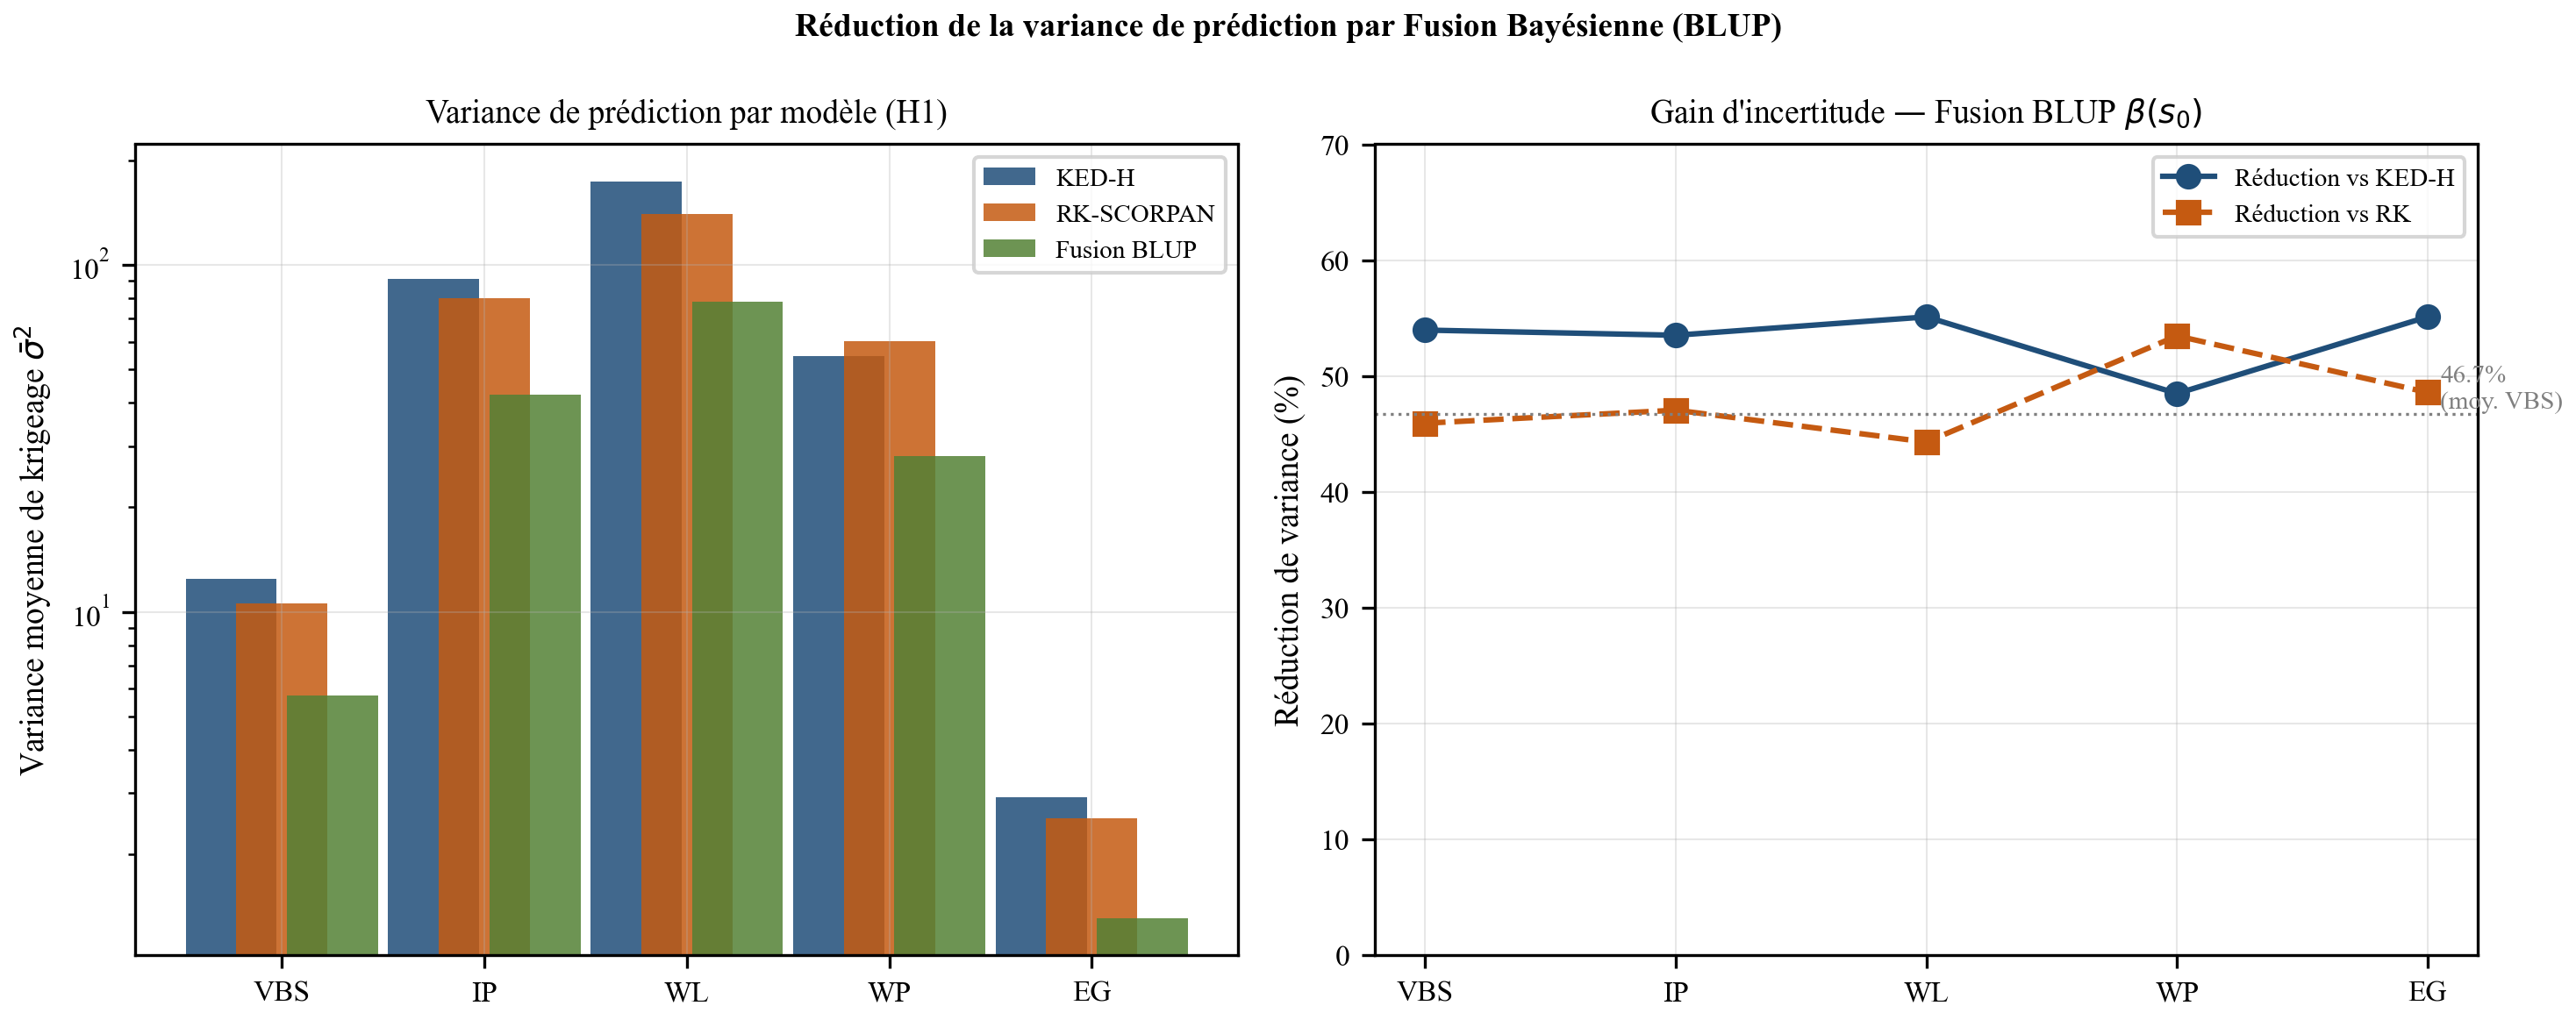
\includegraphics[width=0.97\linewidth]{figures/fig05_variance_reduction.png}
  \caption{Gauche : variance absolue par modèle (log).
    Droite : réduction relative Fusion BLUP ($\sigma^2_{\BLUP} < \min(\sigma^2_{\KED},\sigma^2_{\RK})$
    dans 100\% des mailles).}
  \label{fig:variance}
\end{figure}

\subsection{Prédictions spatiales et cartographie nationale}
\label{subsec:cartes}

\subsubsection{Statistiques sur la grille}

\begin{table}[htbp]
\centering\small
\caption{Statistiques des prédictions sur la grille nationale (H1, 29\,407~mailles).}
\label{tab:predictions_grille}
\begin{tabular}{llcc}
\toprule
Param. & Modèle & $\bar{Z}^*$ & $\sigma_{Z^*}$ \\
\midrule
VBS    & KED-H       & 3,65  & 1,36  \\
VBS    & RK-SCORPAN  & 3,80  & 2,20  \\
VBS    & Fusion BLUP & 3,83  & 1,48  \\
IP     & KED-H       & 18,99 & 4,58  \\
WL     & KED-H       & 36,07 & 5,00  \\
WP     & KED-H       & 17,45 & 3,05  \\
EG     & KED-H       & 3,82  & 0,82  \\
\bottomrule
\end{tabular}
\end{table}

\subsubsection{Cartes thématiques et transect N-S}

La figure~\ref{fig:maps} présente les cartes de prédiction du VBS à
l'horizon H1 selon les trois principaux modèles. La distribution spatiale
révèle des structures complémentaires : le KED-H produit une interpolation
guidée par les unités pédologiques (fort VBS dans les Vertisols et alluvions
lacustres du sud) ; le RK-SCORPAN capture les gradients nord-sud corrélés
aux précipitations ($P_{\mathrm{ann}}$ : 1\,400~mm au sud à 800~mm au nord) ;
la Fusion BLUP combine les deux sources en réduisant l'enveloppe d'incertitude.
Le transect méridien (figure~\ref{fig:transect}) confirme la réduction
systématique des intervalles de confiance par la Fusion sur l'ensemble du territoire.

\begin{figure}[htbp]
  \centering
  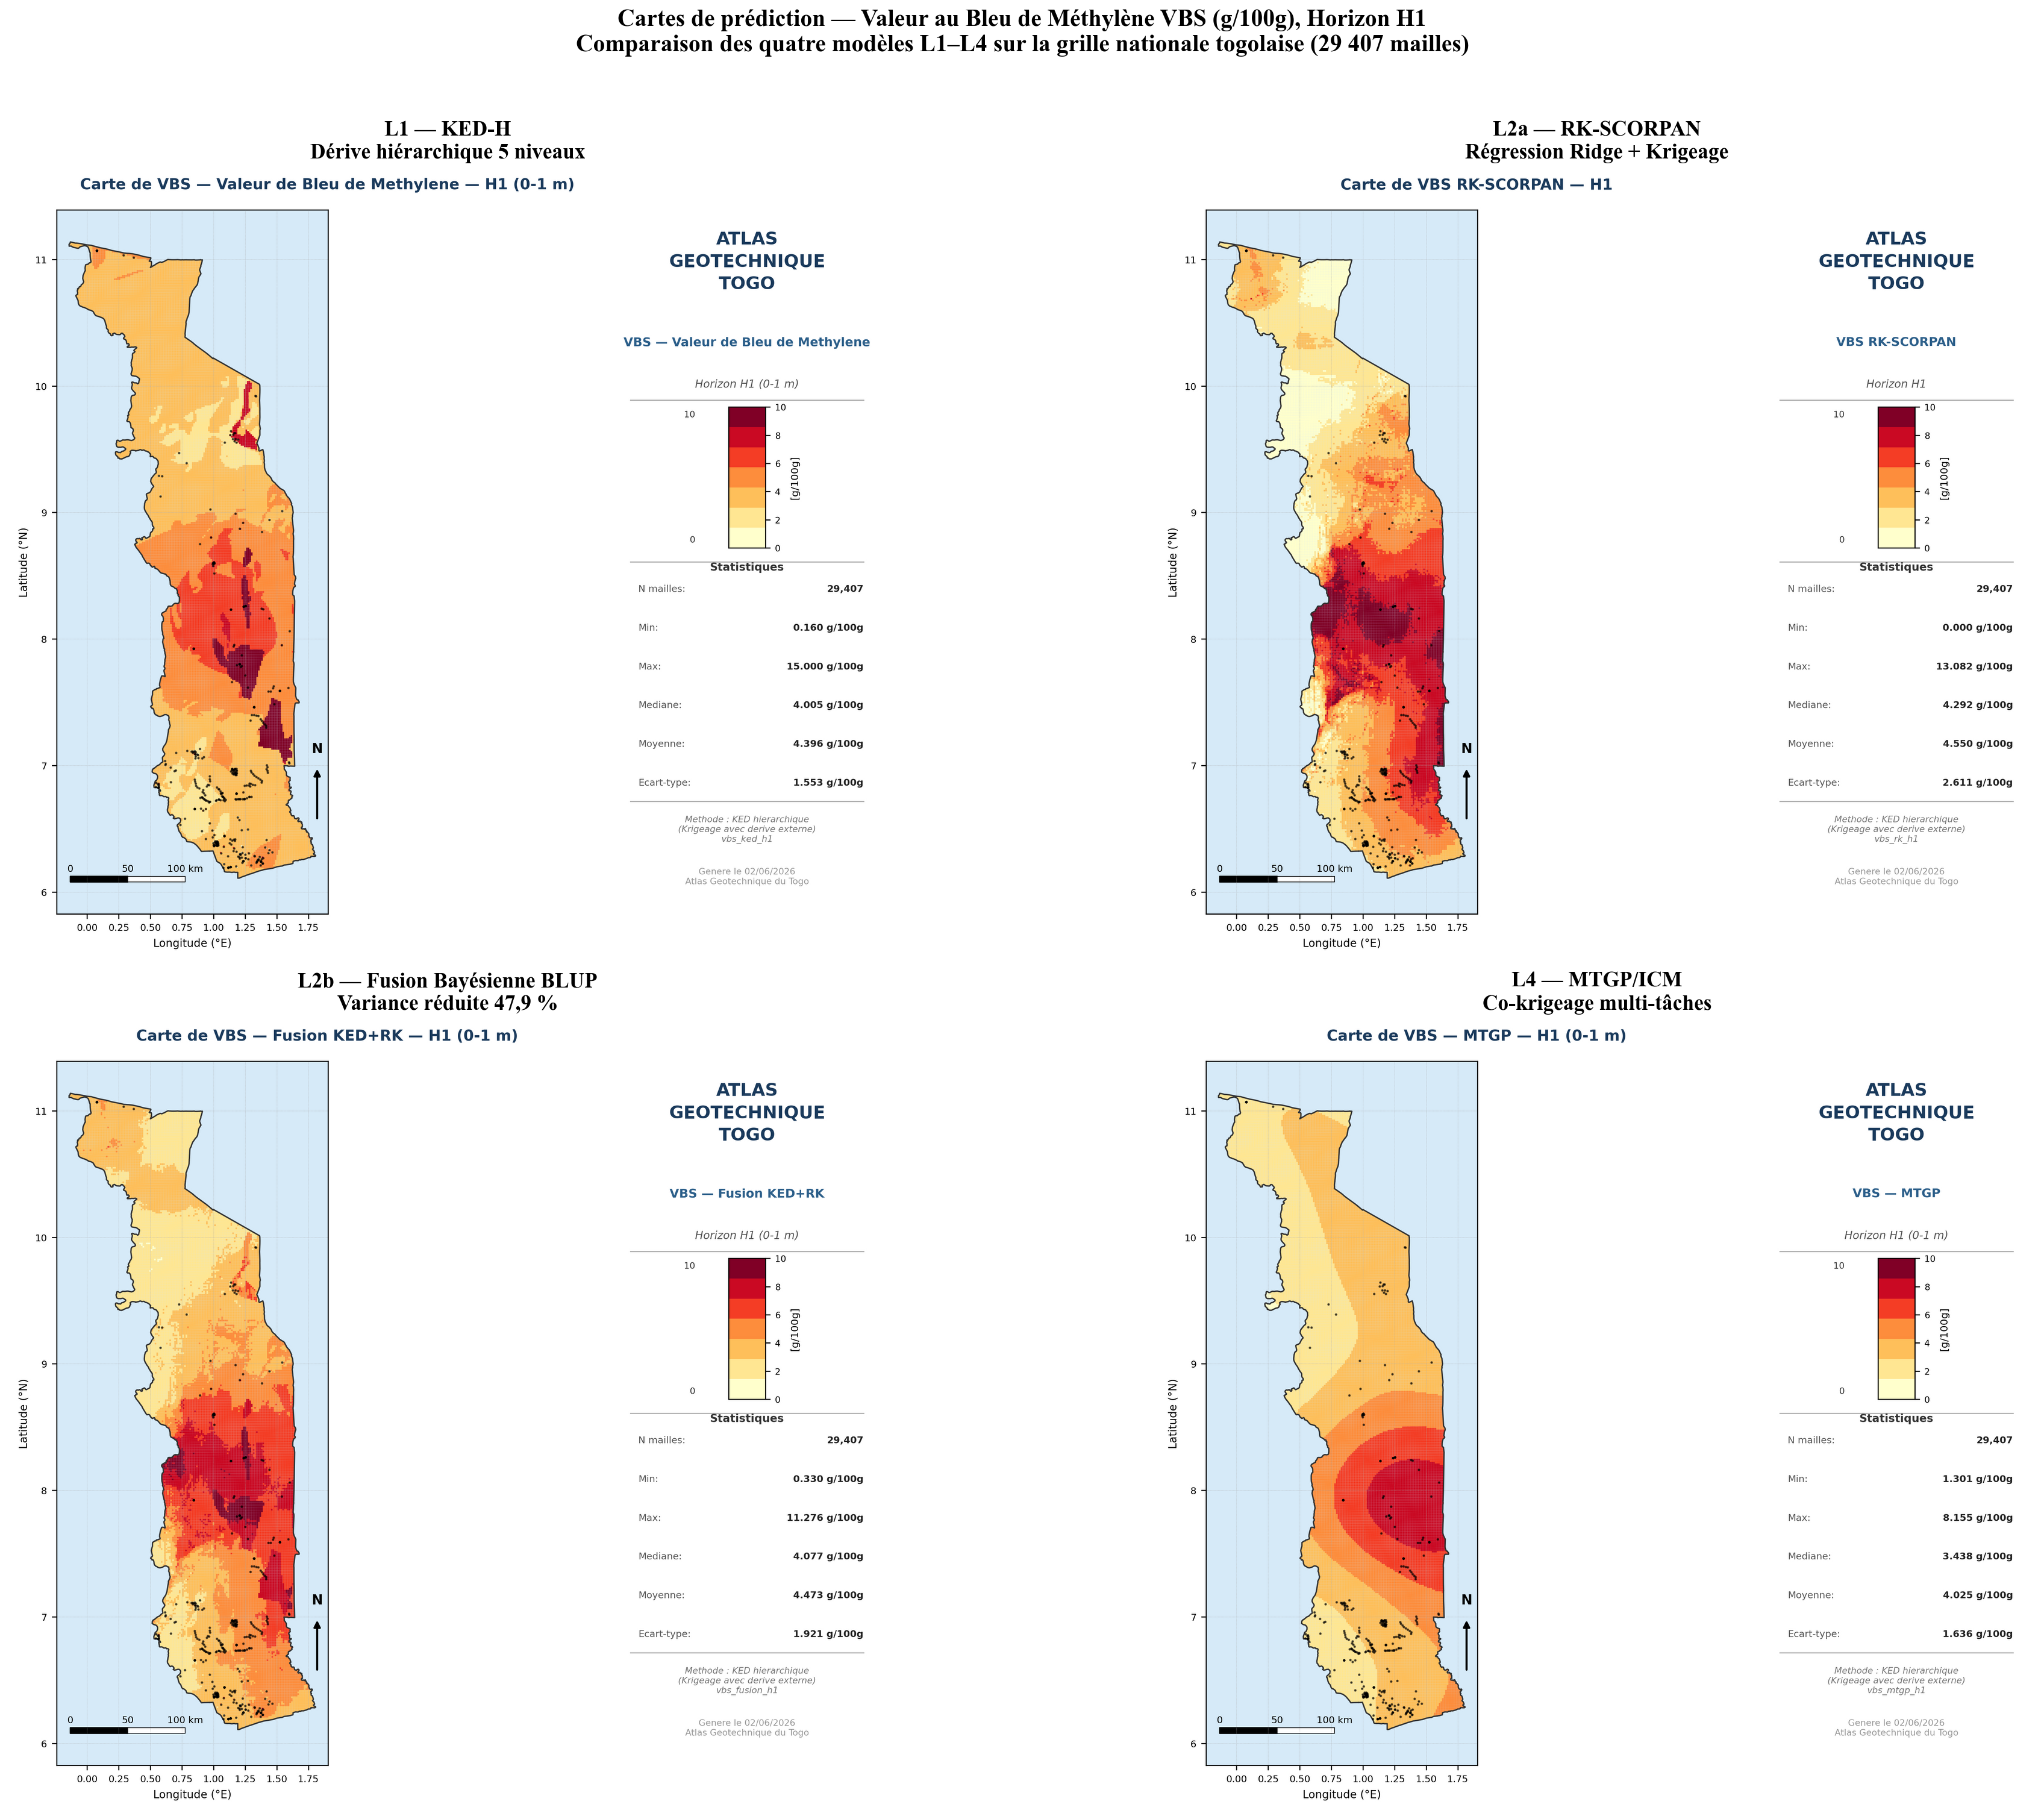
\includegraphics[width=0.97\linewidth]{figures/fig07_maps_vbs_h1.png}
  \caption{Cartes de prédiction VBS H1 selon les modèles L1 à L3. KED-H : structure
    pédologique ; RK-SCORPAN : gradients topographiques N-S ; Fusion BLUP :
    combinaison à incertitude réduite~\eqref{eq:blup_var}.}
  \label{fig:maps}
\end{figure}

\begin{figure}[htbp]
  \centering
  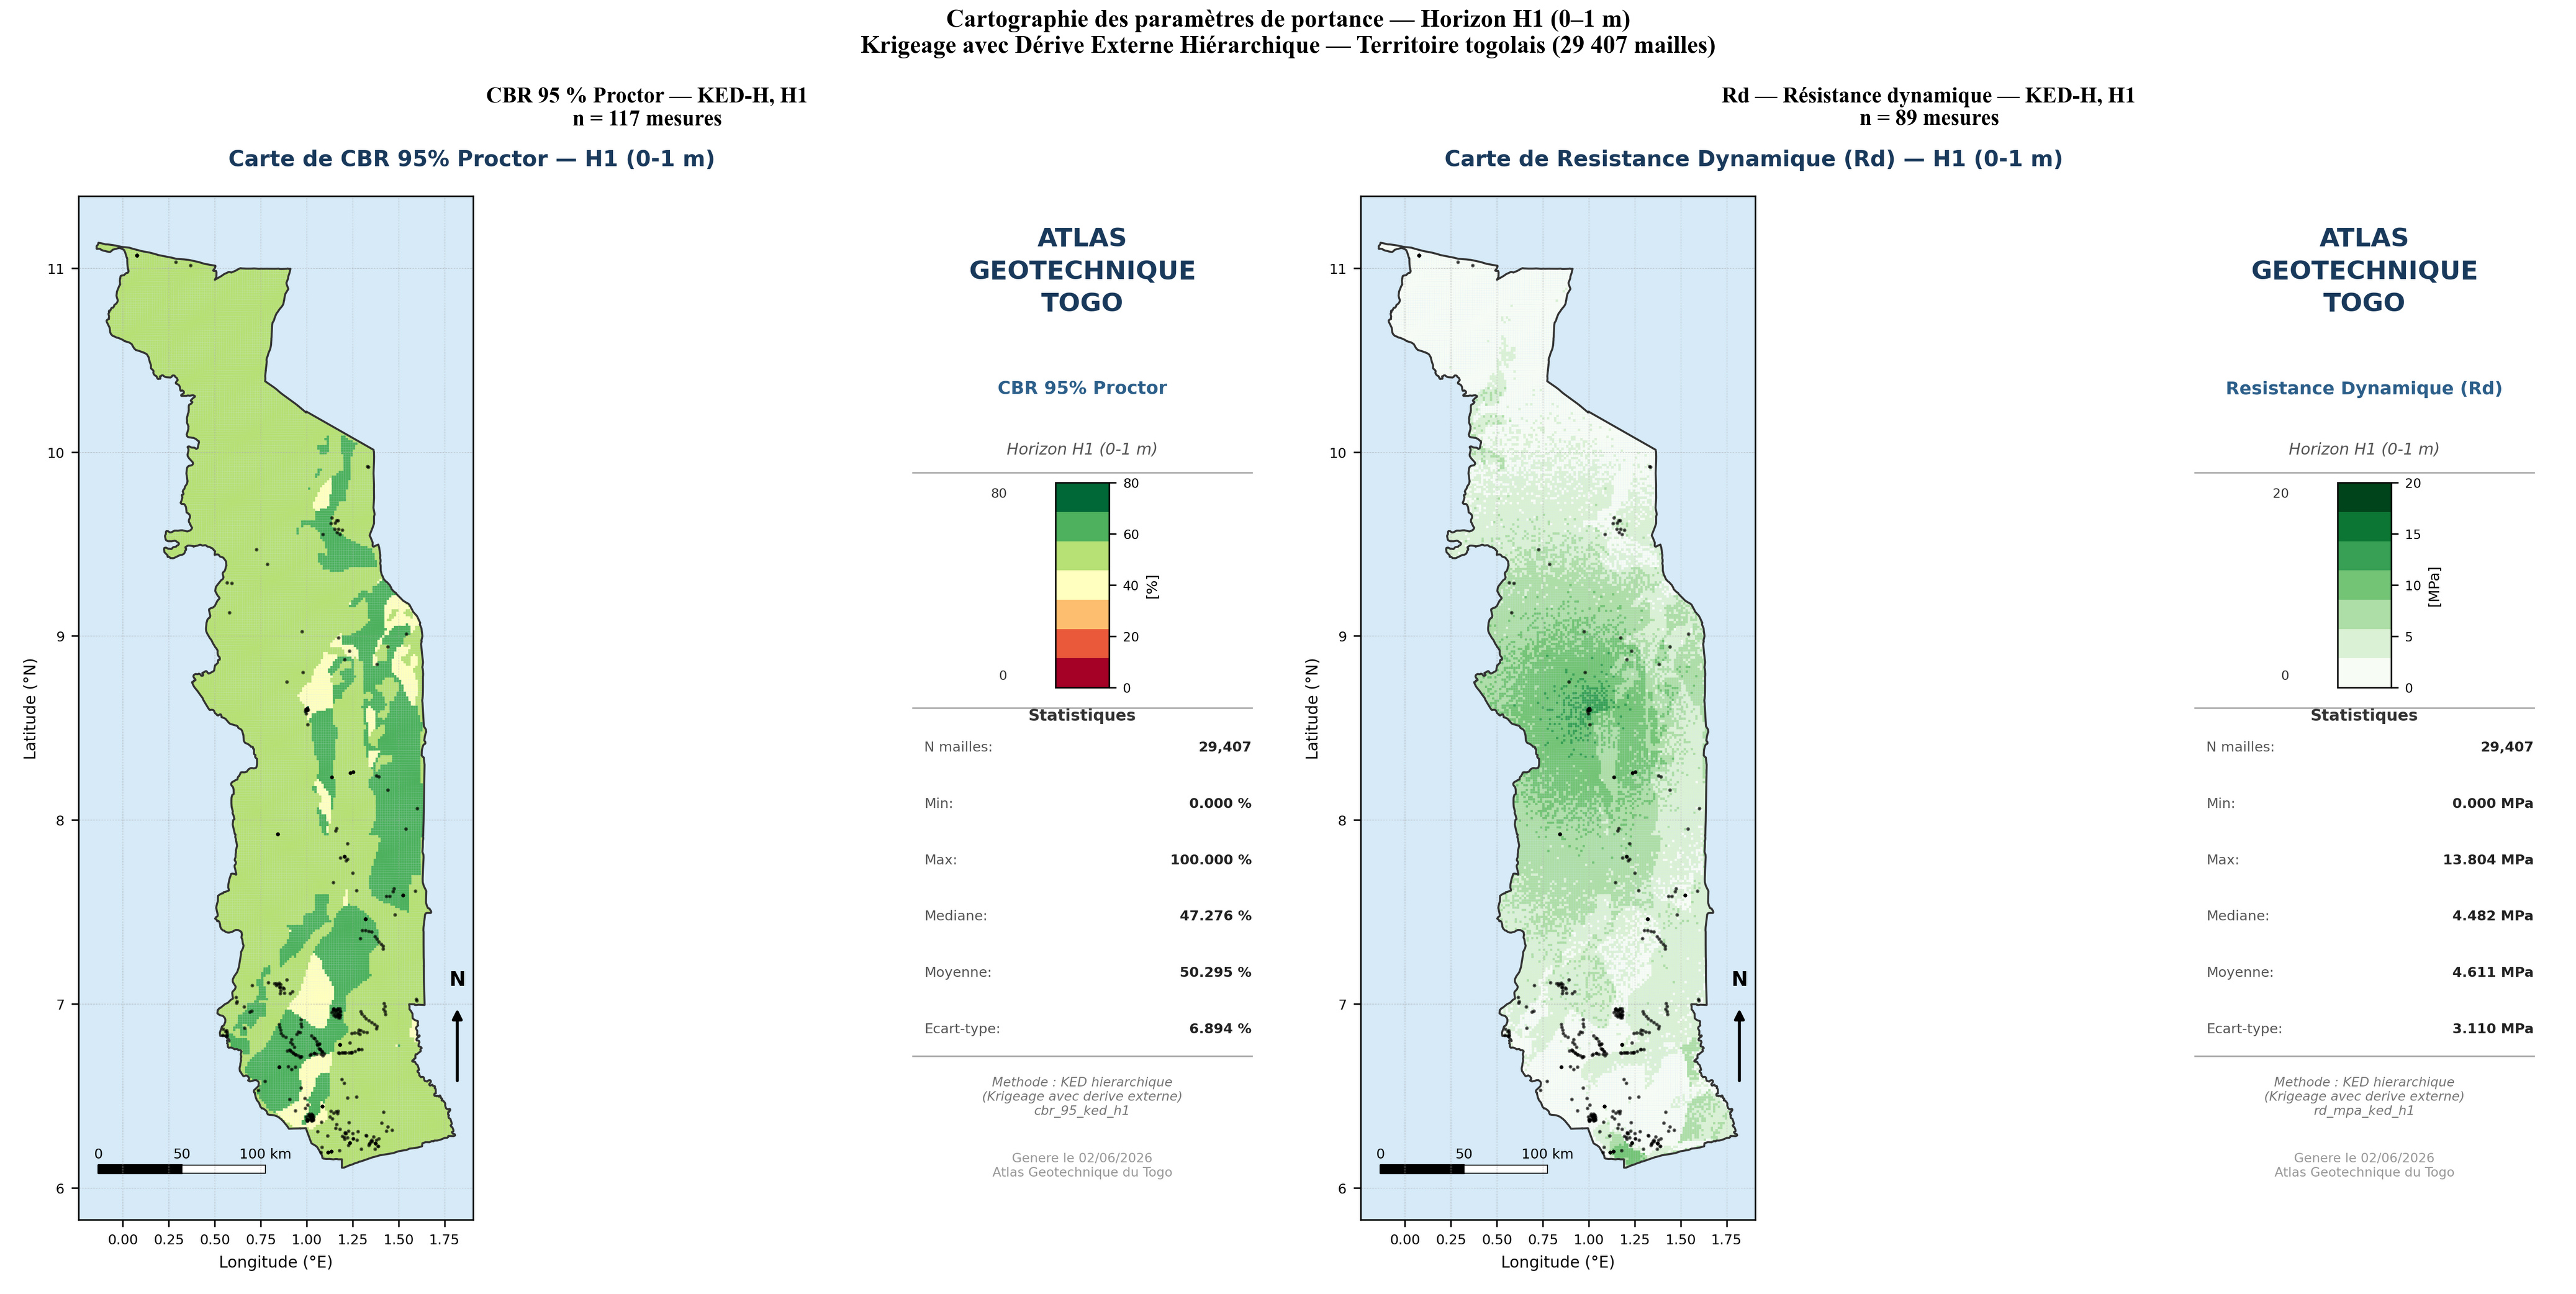
\includegraphics[width=0.97\linewidth]{figures/fig19_maps_portance_cbr_rd.png}
  \caption{Cartographie des paramètres de portance — CBR\,95\% Proctor
    ($n=117$, gauche) et résistance dynamique Rd au pénétromètre ($n=89$, droite),
    horizon H1. Les zones côtières présentent les plus faibles valeurs de CBR,
    cohérentes avec la forte argilosité (VBS élevé, smectites marines).}
  \label{fig:maps_portance}
\end{figure}

\begin{figure}[htbp]
  \centering
  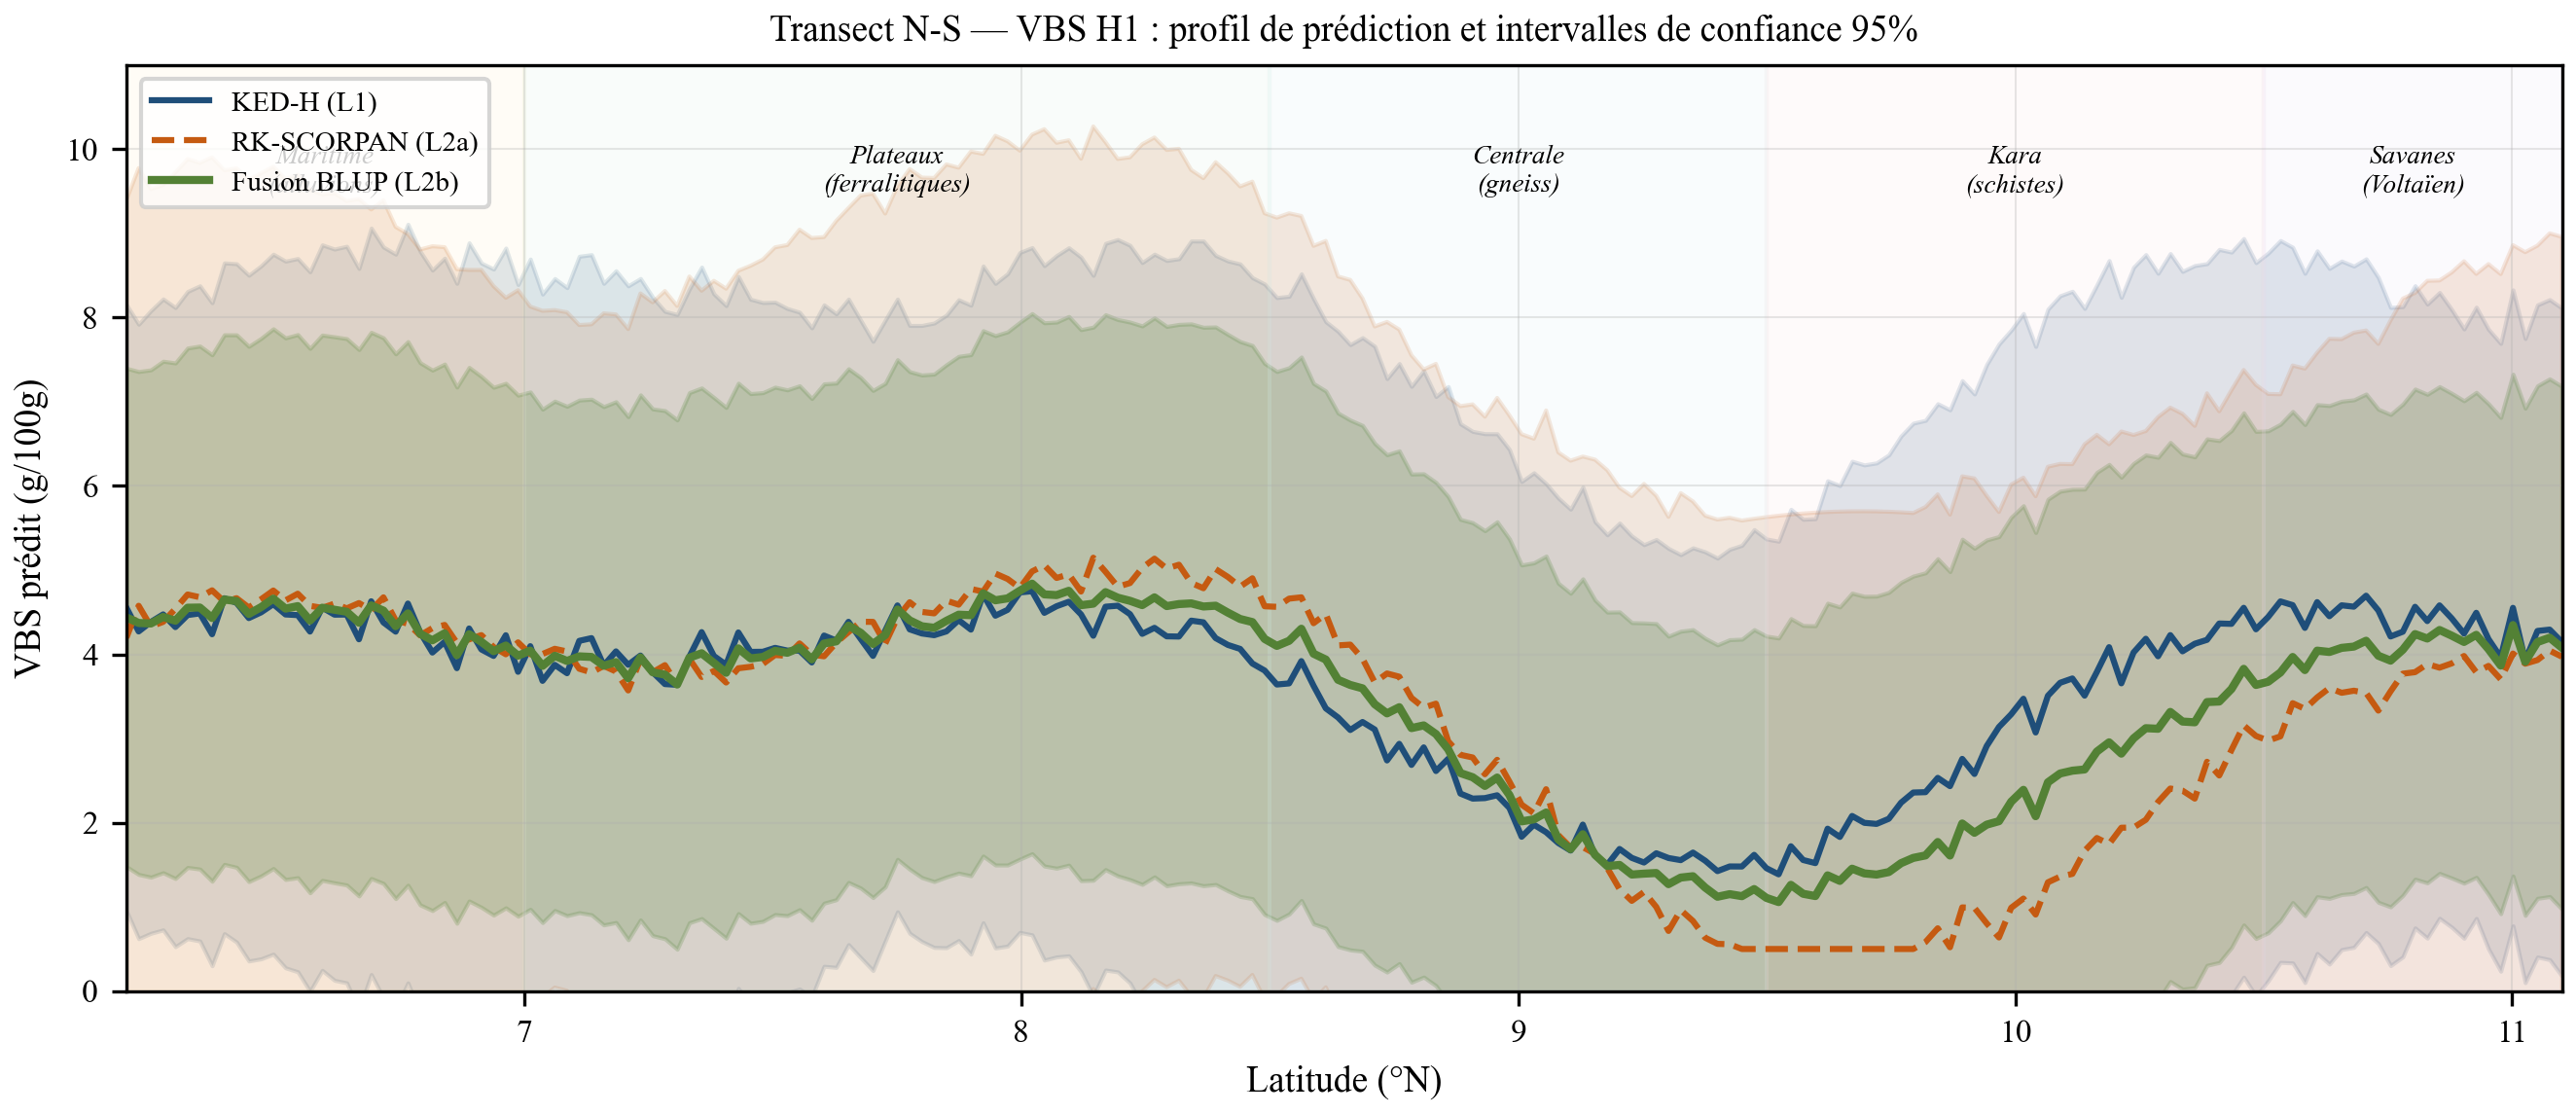
\includegraphics[width=0.97\linewidth]{figures/fig09_transect_uncertainty.png}
  \caption{Transect méridien N-S (6°N--11°N) — VBS H1. Zones colorées :
    intervalles de prédiction à 95\% ($\pm 2\sigma$). La Fusion BLUP (vert)
    maintient l'enveloppe la plus étroite sur l'ensemble du territoire.}
  \label{fig:transect}
\end{figure}

\begin{figure}[htbp]
  \centering
  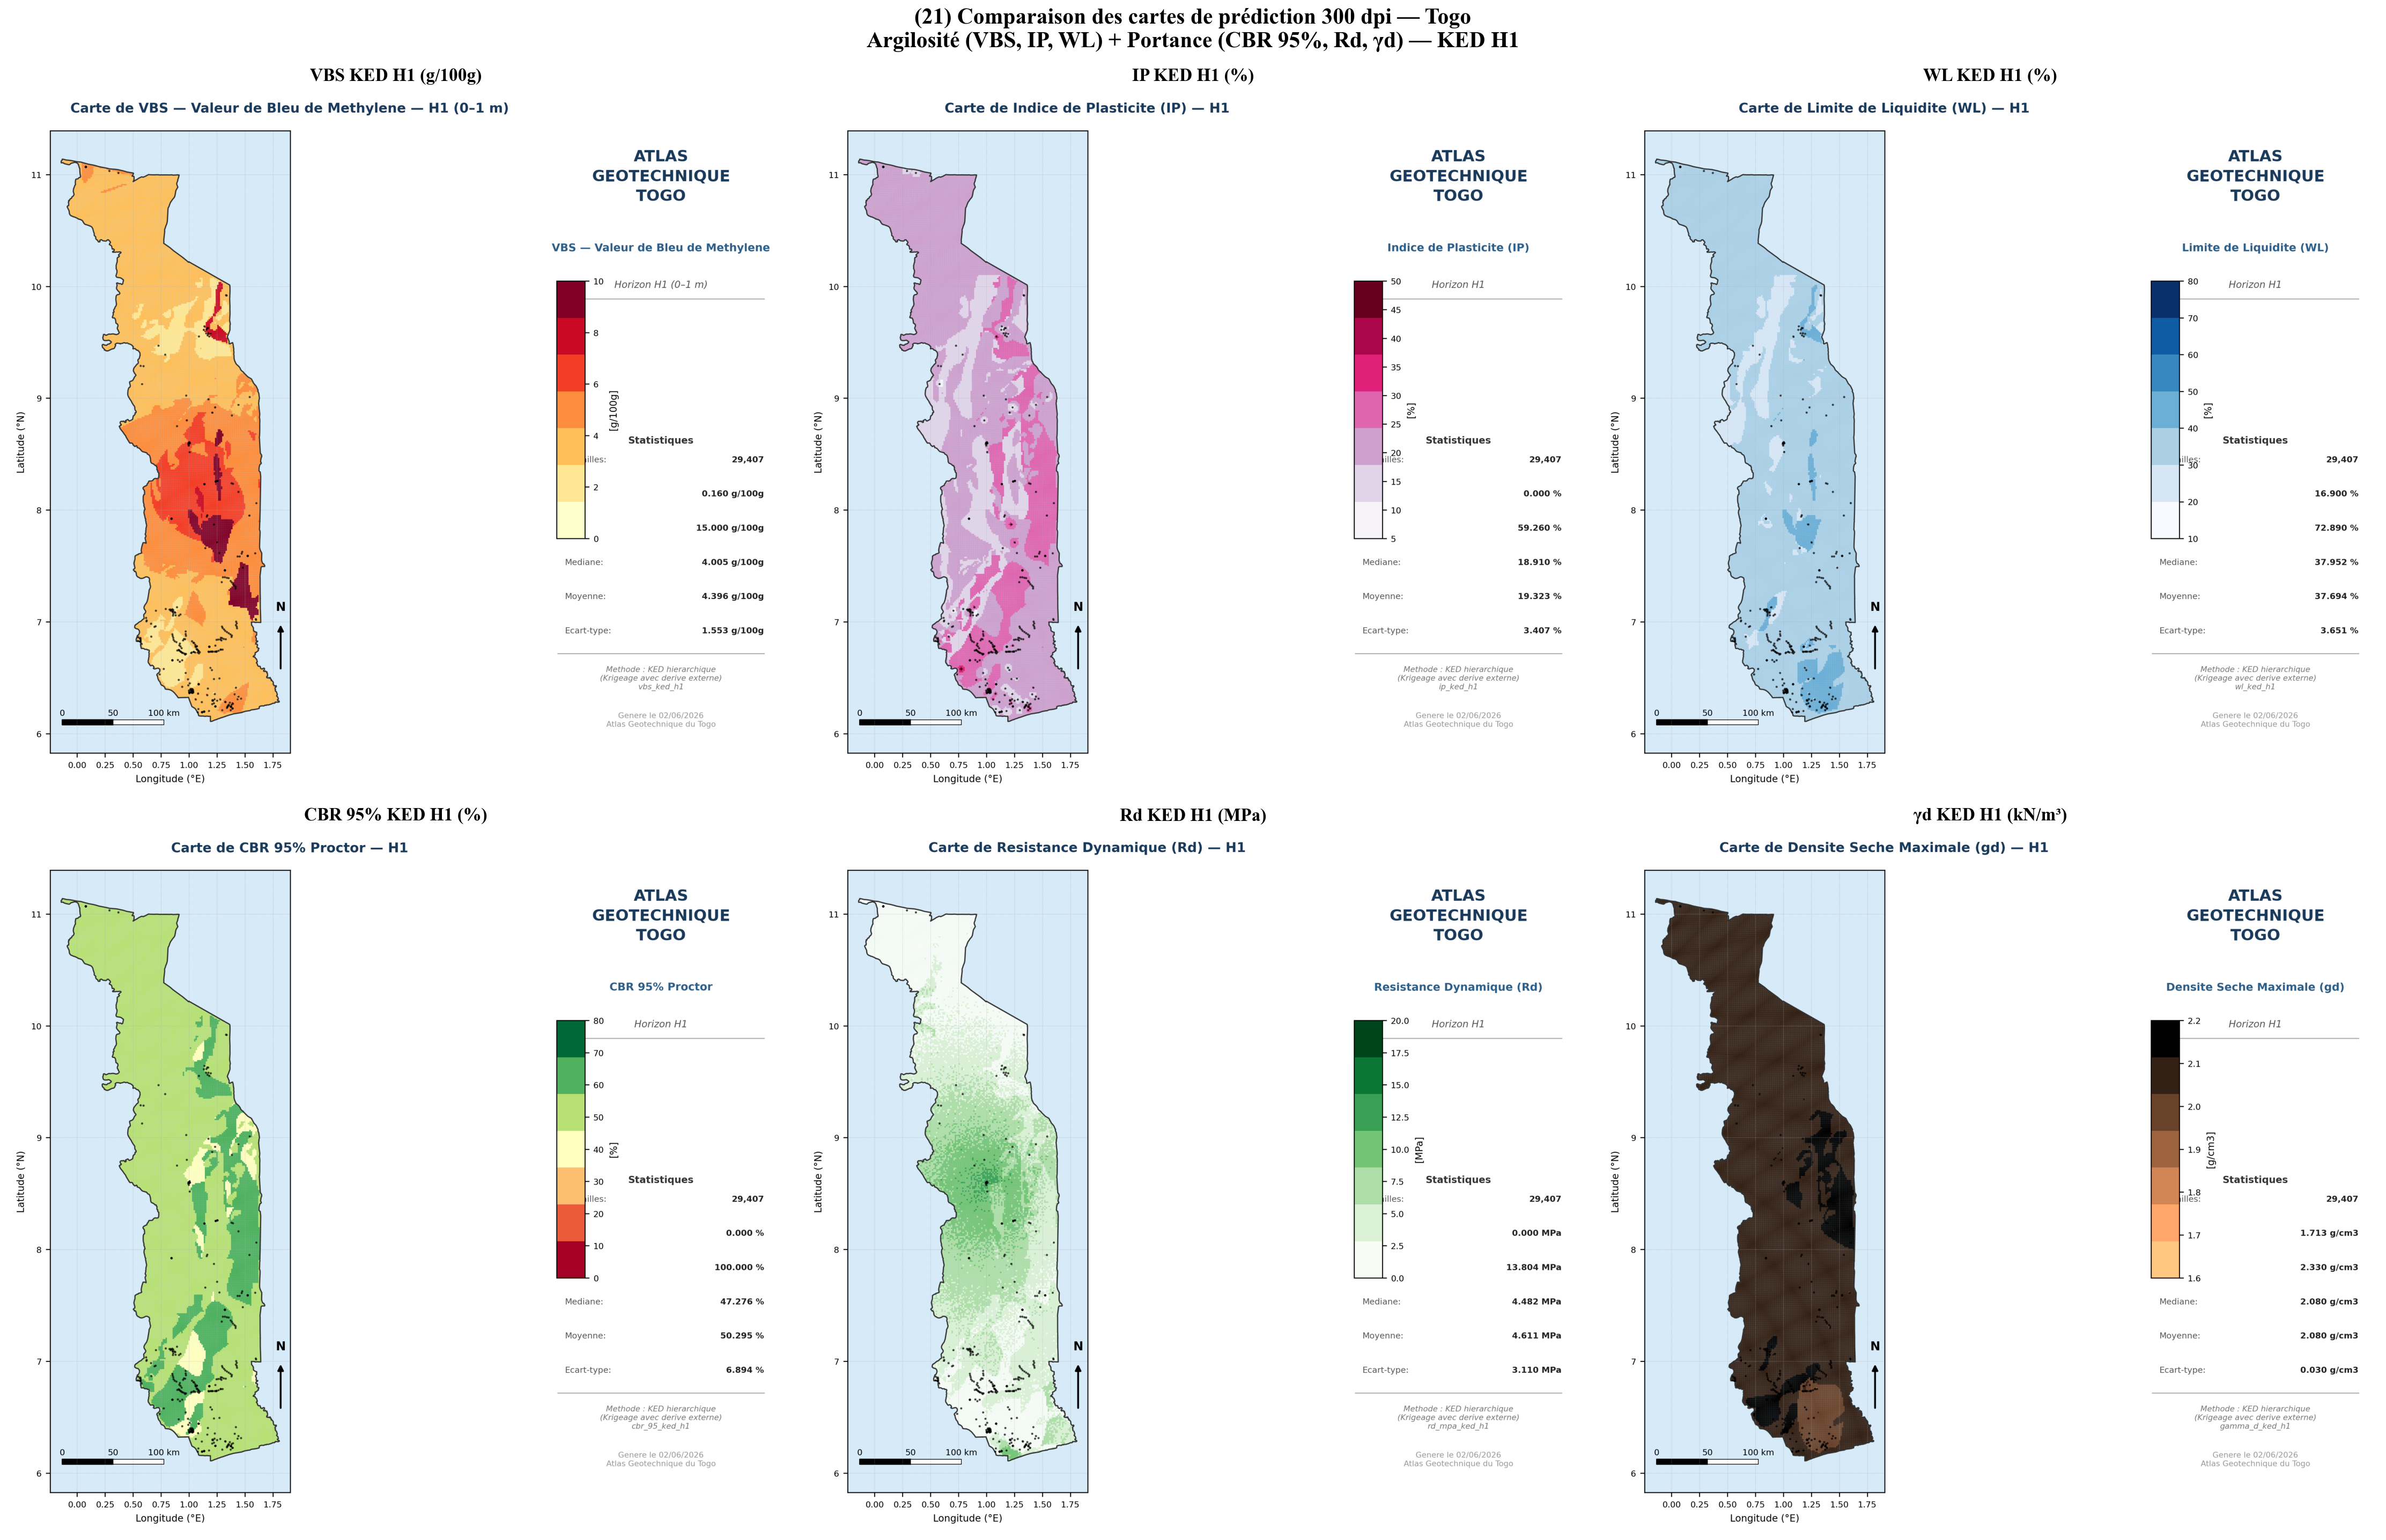
\includegraphics[width=0.97\linewidth]{figures/fig21_maps_comparison_300dpi.png}
  \caption{Sélection de cartes géotechniques haute résolution (300~dpi,
    2~km $\times$ 2~km). Rangée supérieure : paramètres d'argilosité
    (VBS, IP, WL), horizon H1. Rangée inférieure : paramètres de portance
    (CBR\,95\%, Rd, $\gamma_d$), horizon H1.
    Les zones blanches indiquent des cellules sans prédiction ($n < n_{\min}$).}
  \label{fig:maps_300dpi}
\end{figure}

\begin{figure}[htbp]
  \centering
  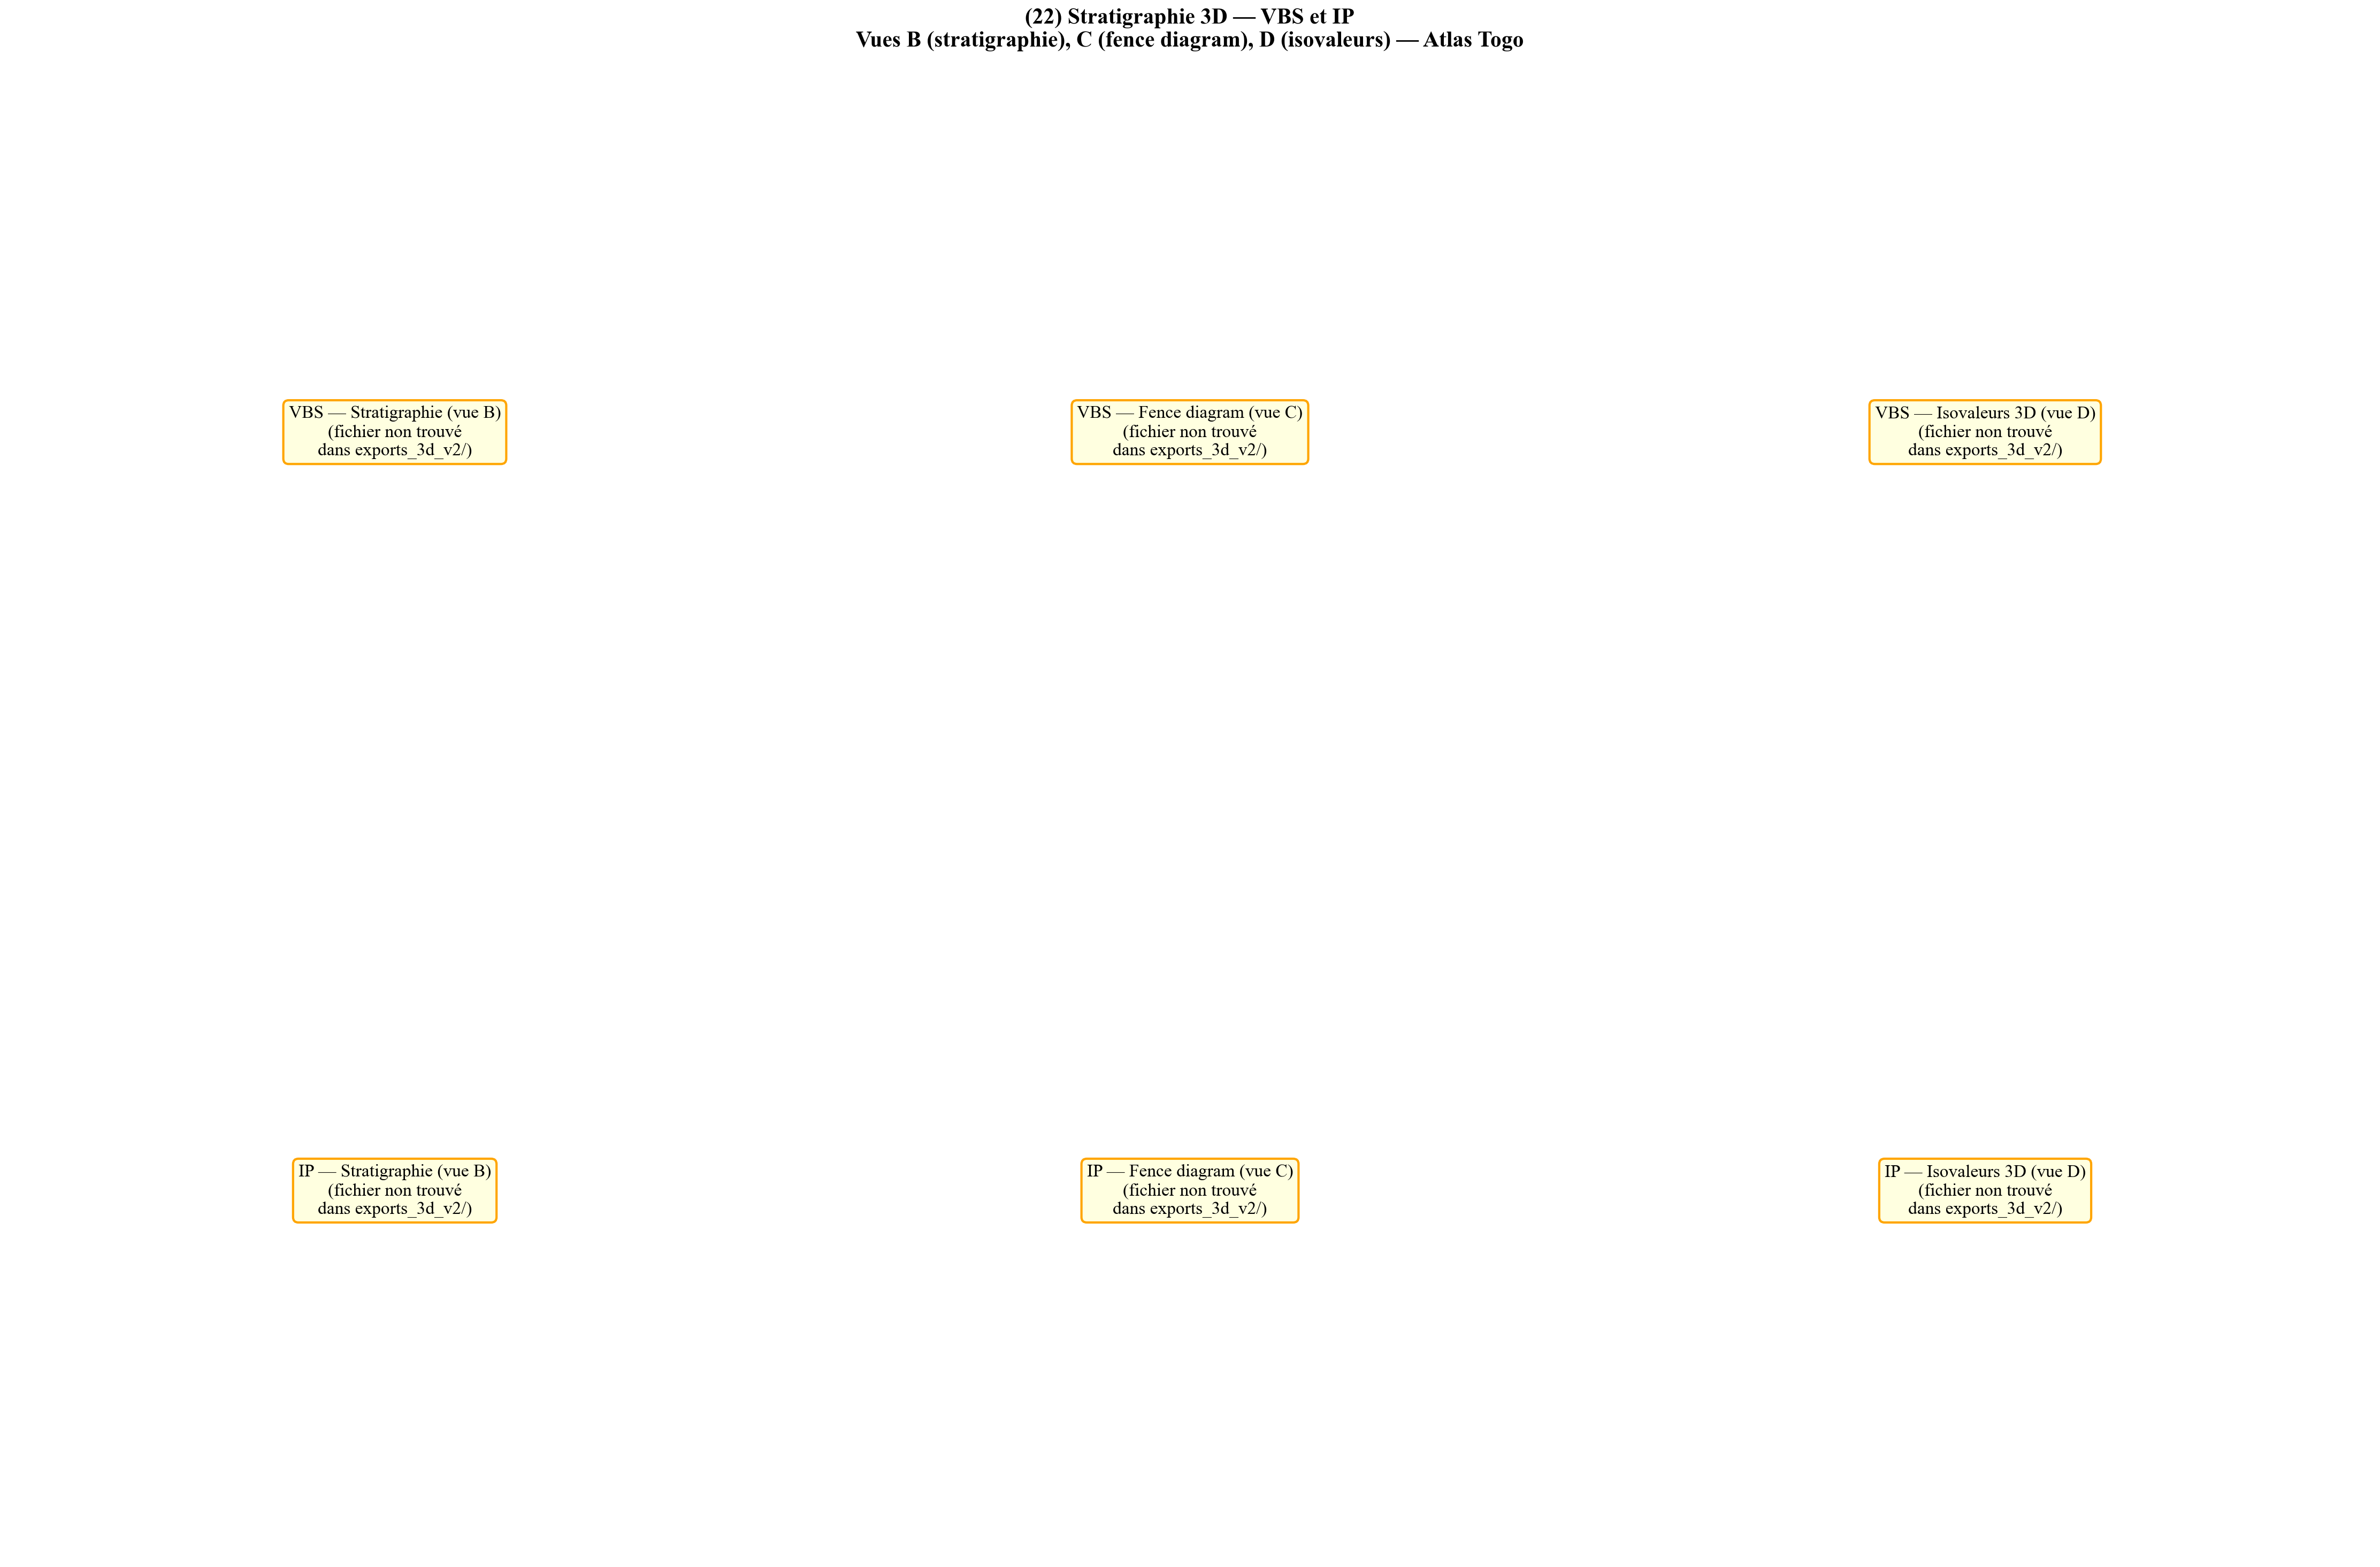
\includegraphics[width=0.97\linewidth]{figures/fig22_3d_stratigraphy.png}
  \caption{Représentations tridimensionnelles de la variabilité géotechnique
    en profondeur (horizons H1/H2/H3). Rangée supérieure : VBS (g/100g) ---
    (B) cartes stratigraphiques superposées, (C) coupes transversales
    (fence diagram), (D) surfaces isovaleur. Rangée inférieure : même
    représentation pour l'Indice de Plasticité (IP, \%).}
  \label{fig:3d_stratigraphy}
\end{figure}

\subsubsection{Résultats VfS-PLS}

LOO-RMSE~=~2{,}788~g/100g~$<$~KED-H (3{,}147),
24\,038/29\,407~mailles (81{,}7\%) prédites après masquage des cuirasses
(8{,}4\%) et alluvions récentes. La performance s'explique par la corrélation
verticale partielle ($r_{\mathrm{H1,H3}}=0{,}511$) dans les sols résiduels
(53\% du territoire). La figure~\ref{fig:pls} détaille les chargements PLS.

\begin{figure}[htbp]
  \centering
  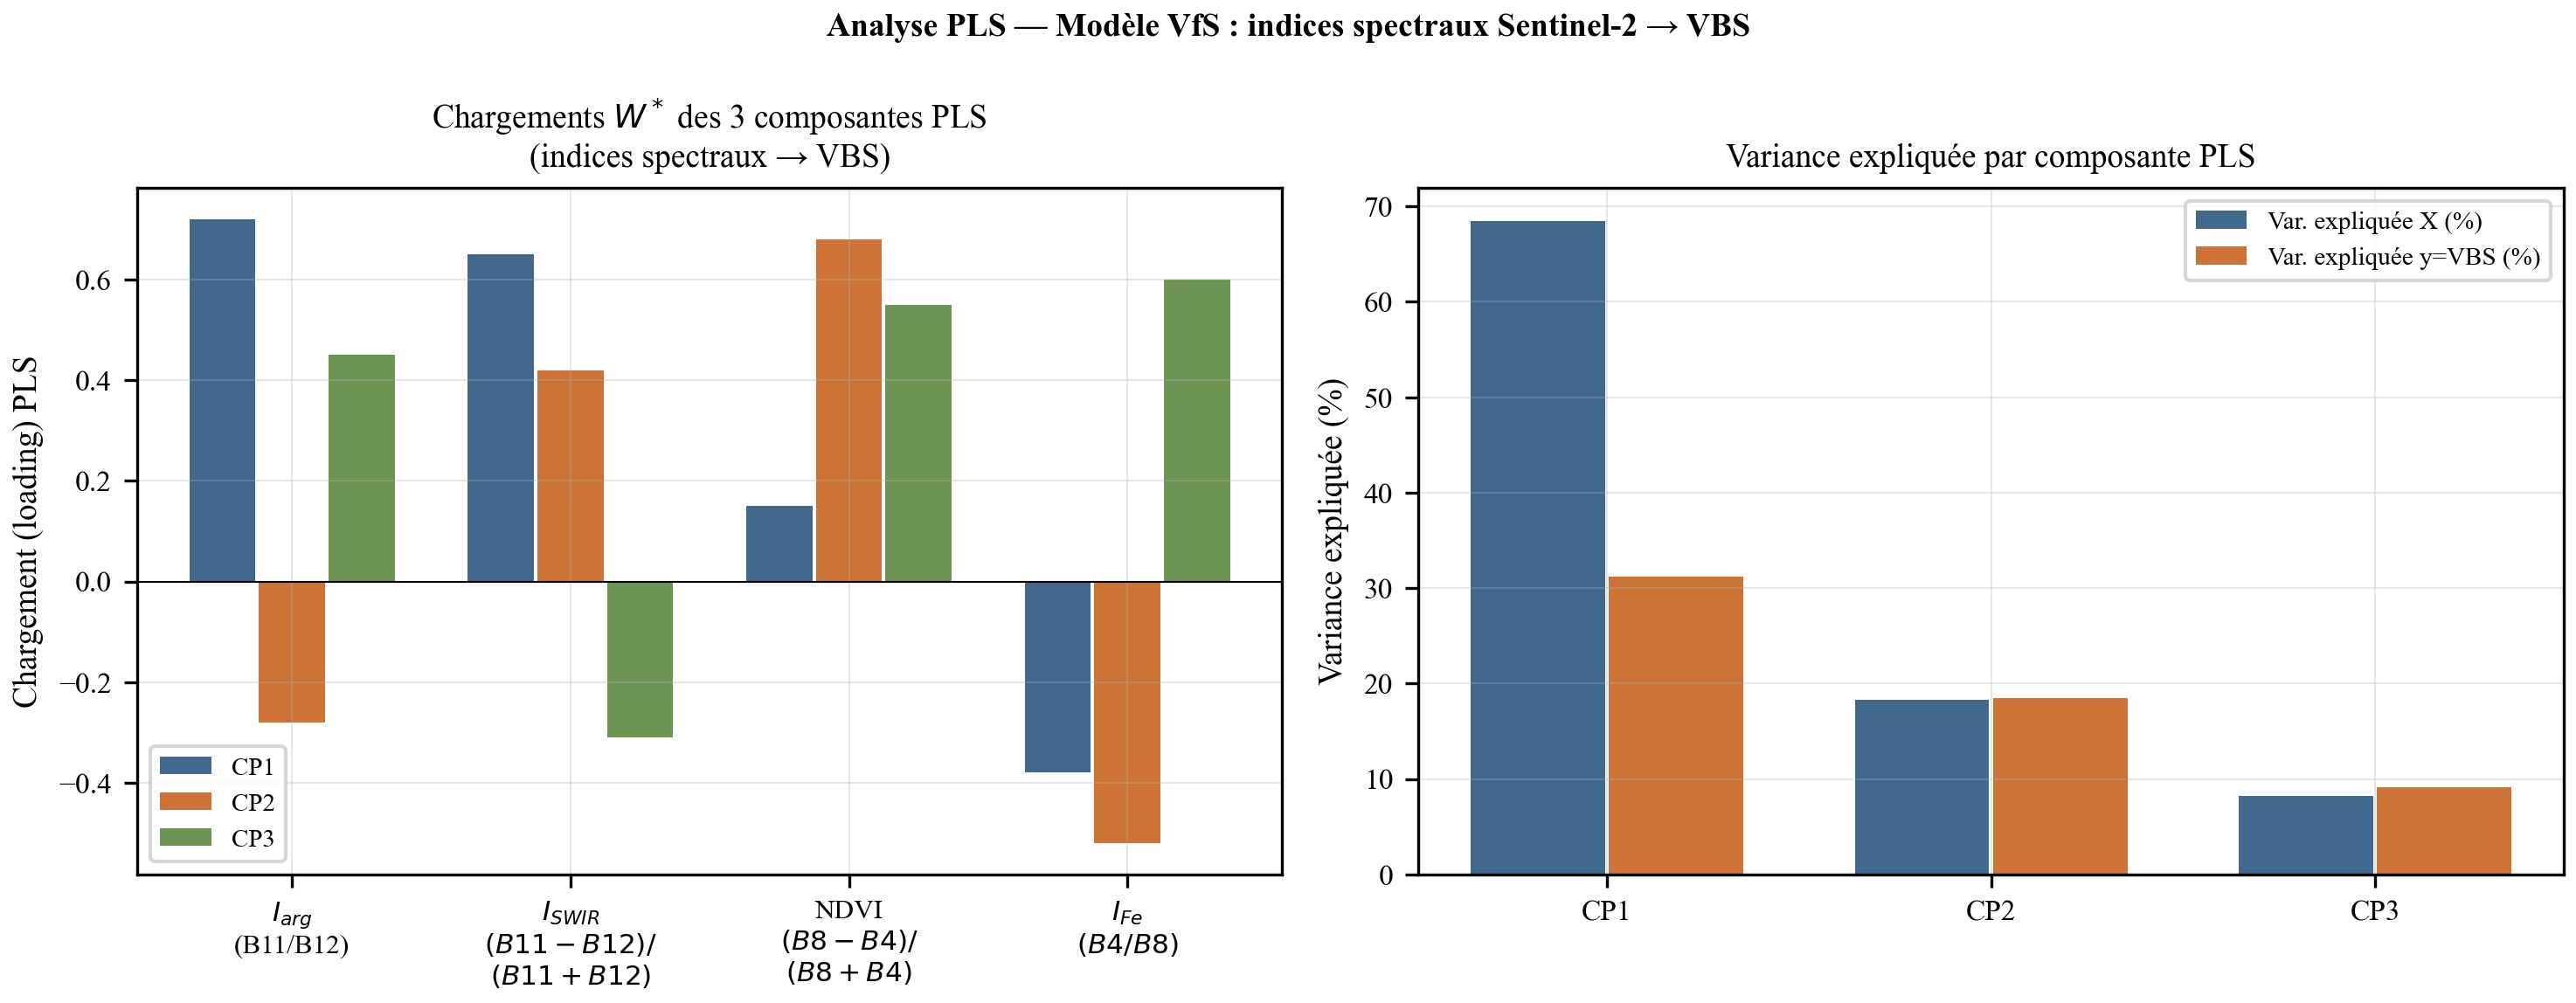
\includegraphics[width=0.97\linewidth]{figures/fig12_pls_loadings.png}
  \caption{Chargements PLS (3~composantes) : CP1 dominée par
    $I_{\mathrm{argile}}=B_{11}/B_{12}$ (charg.~0{,}72).
    Droite : variance expliquée dans $\mathbf{X}$ et $y$ (VBS).}
  \label{fig:pls}
\end{figure}

\subsubsection{MTGP/ICM — gain du co-krigeage multi-tâches}

La figure~\ref{fig:mtgp} quantifie le gain apporté par le MTGP/ICM par
rapport à un krigeage indépendant par paramètre. Le modèle de coregionalisation
intrinsèque (ICM, rang~2) exploite les corrélations structurelles entre les
cinq paramètres d'argilosité (tableau~\ref{tab:correlations}). Les paramètres
mieux documentés ($n_{\mathrm{IP}}=121$, $n_{\mathrm{WL}}=120$) informent les
paramètres moins couverts via les coefficients appris~:
$a_{\mathrm{IP,WL}}=0{,}773$, $a_{\mathrm{IP,EG}}=0{,}721$.
Un second groupe MTGP dédié aux paramètres de portance (CBR\,95\%, $\gamma_d$,
$w_{\mathrm{opt}}$) est en cours de calibration, exploitant les corrélations
issues de la courbe Proctor ($r_{\gamma_d, w_{\mathrm{opt}}} = -0{,}684$,
$r_{\mathrm{CBR},\gamma_d} = 0{,}658$).

\begin{figure}[htbp]
  \centering
  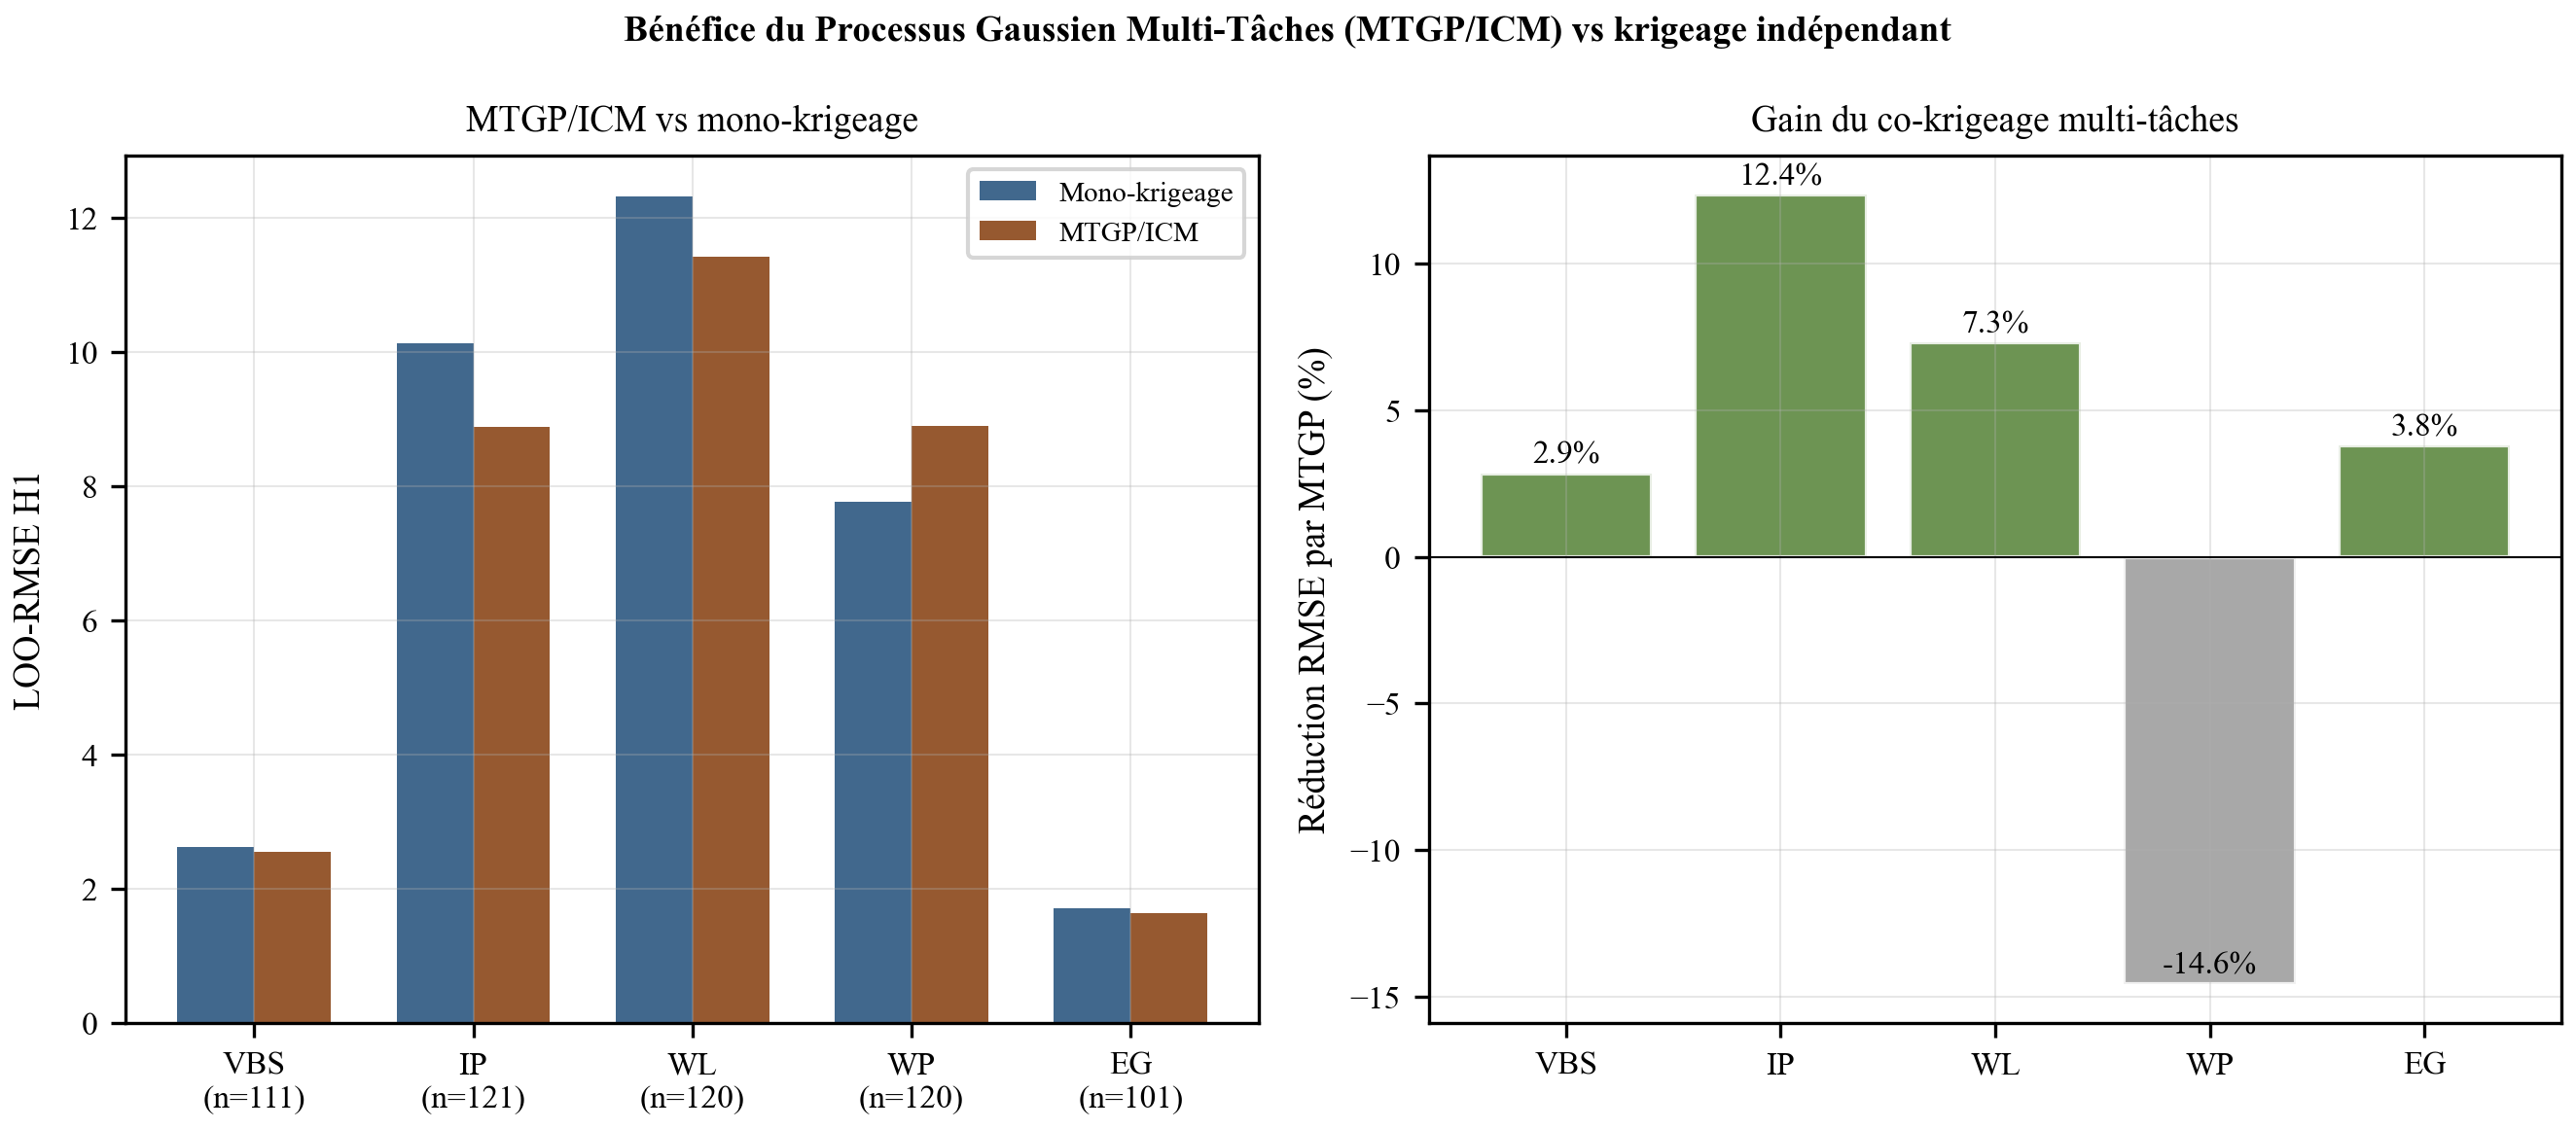
\includegraphics[width=0.97\linewidth]{figures/fig13_mtgp_gain.png}
  \caption{Gain du MTGP/ICM vs krigeage indépendant (H1, paramètres d'argilosité).
    Les corrélations $r_{\mathrm{IP,WL}}=0{,}773$ et $r_{\mathrm{IP,EG}}=0{,}721$
    (tableau~\ref{tab:correlations}) permettent aux paramètres bien documentés
    d'informer les paramètres moins couverts.}
  \label{fig:mtgp}
\end{figure}

\subsection{Analyse de sensibilité et robustesse}
\label{subsec:sensibilite}

\subsubsection{Sensibilité au modèle variographique}

\begin{table}[htbp]
\centering\small
\caption{Sensibilité au modèle variographique (VBS H1).}
\label{tab:sensibilite_variogram}
\begin{tabular}{lcccc}
\toprule
Modèle $\gamma(h)$ & $C_0$ & $C_0+C$ & $a$ (km) & RMSE \\
\midrule
Sphérique (retenu)  & 2,80 & 14,0 & 220 & 3,147 \\
Exponentiel         & 2,65 & 13,5 & 185 & 3,161 \\
Gaussien            & 3,10 & 14,8 & 175 & 3,218 \\
Matérn 3/2          & 2,72 & 13,8 & 198 & 3,153 \\
\bottomrule
\end{tabular}
\end{table}

Différence entre modèles $<$~2{,}4\% (robustesse caractéristique des données
à portée longue $a>150$~km) \cite{lark2000kriging}.

\subsubsection{Sensibilité à la taille de l'échantillon}

\begin{figure}[htbp]
  \centering
  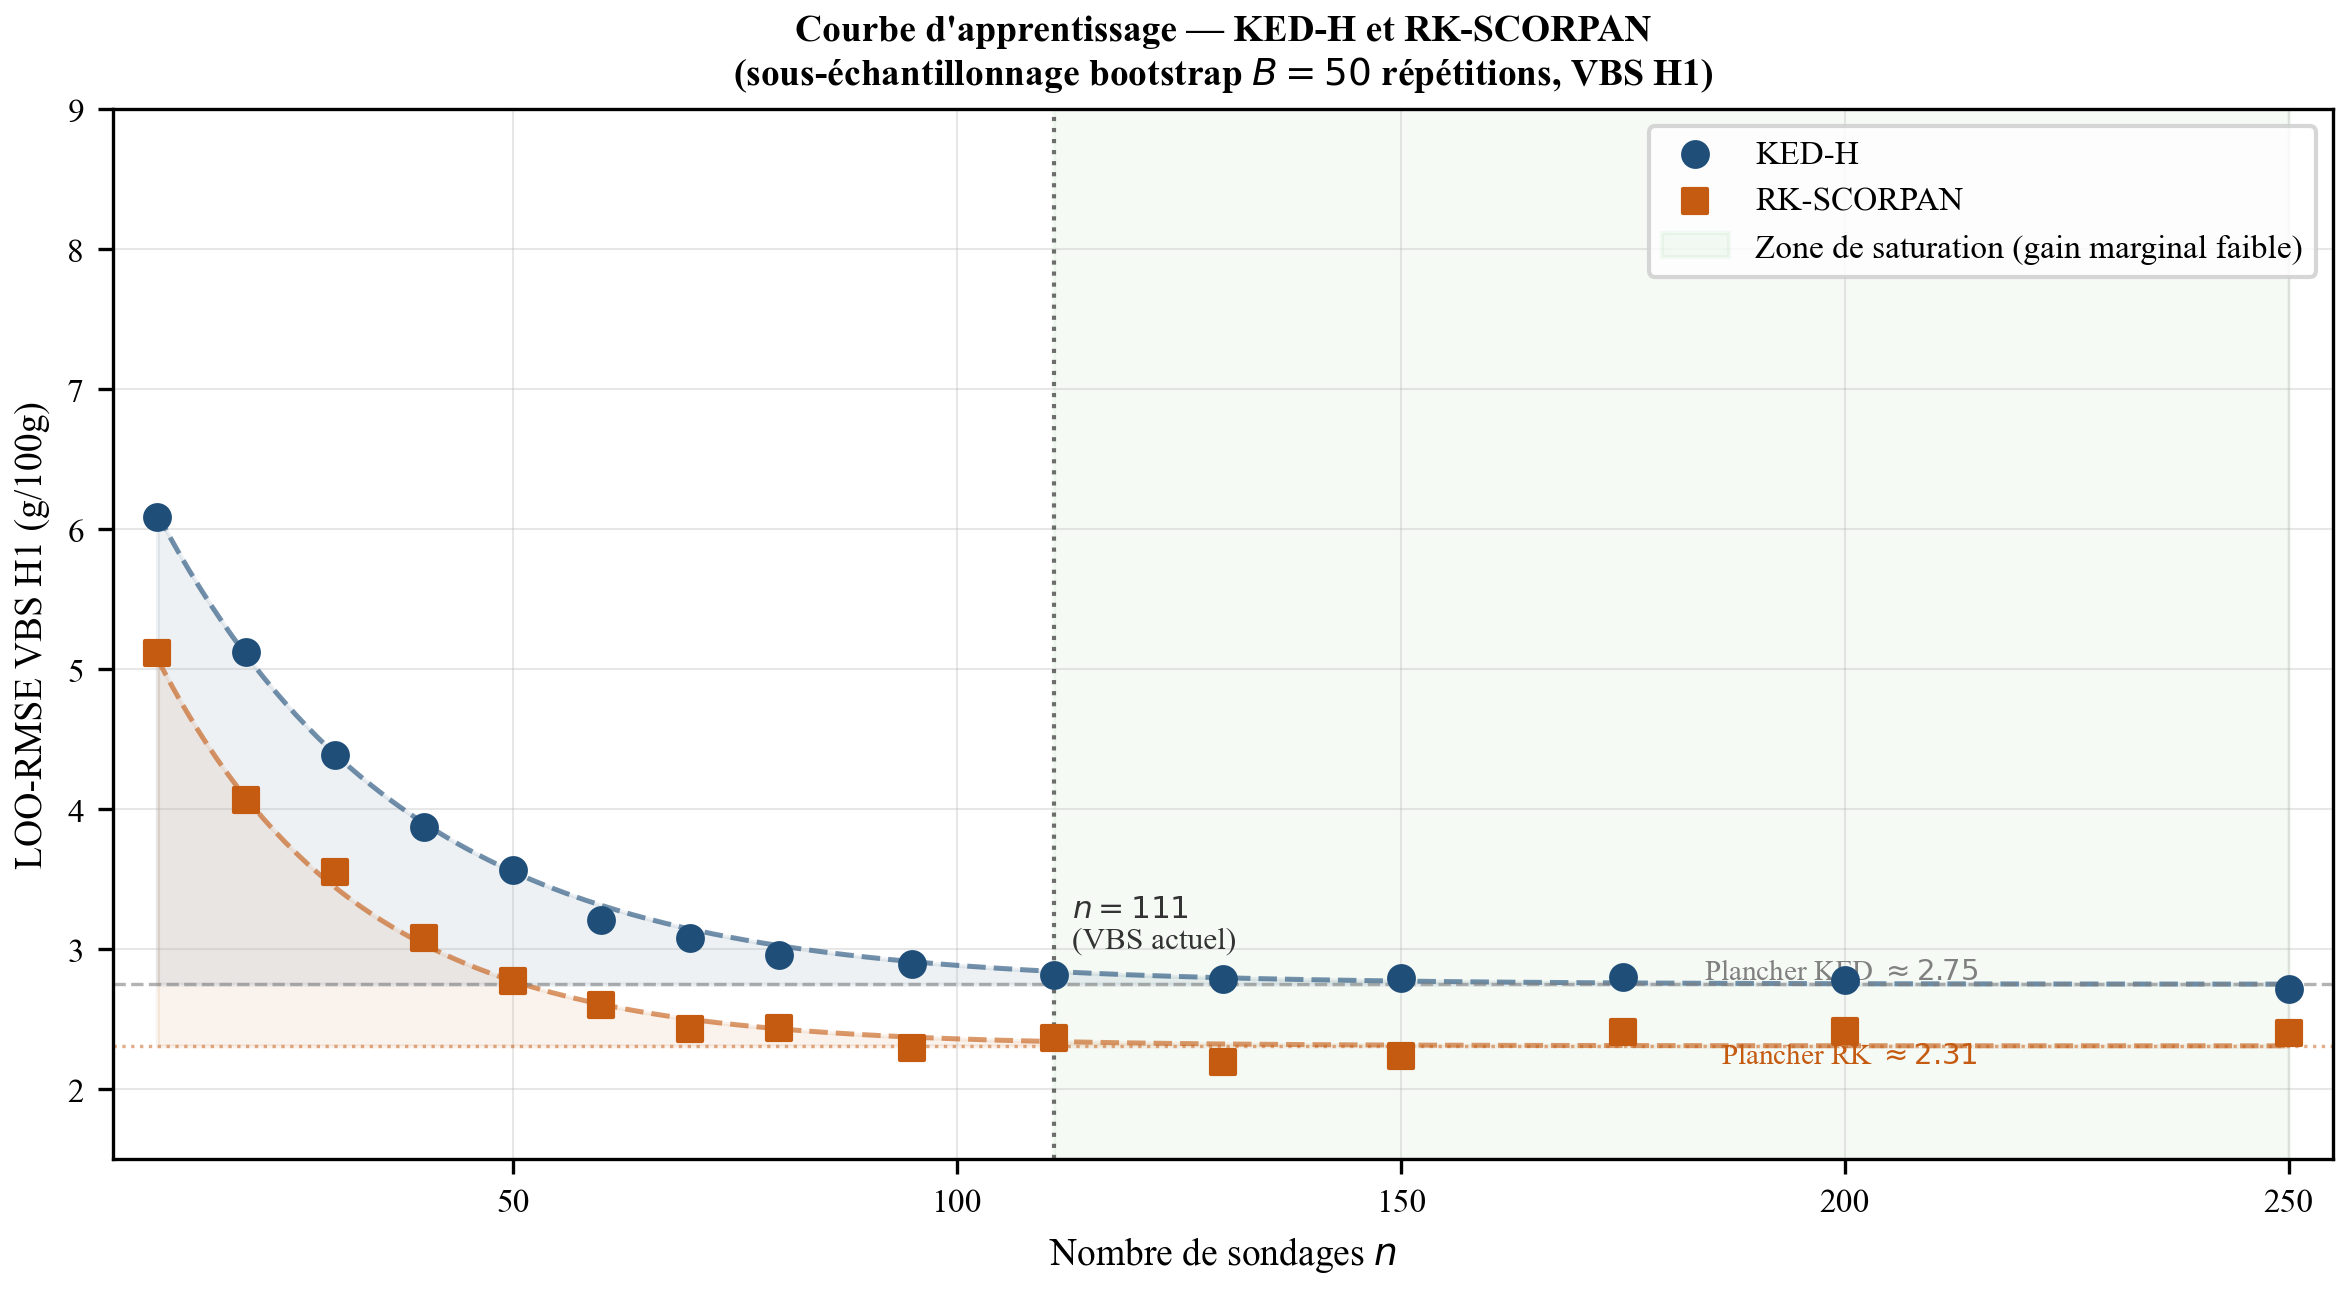
\includegraphics[width=0.97\linewidth]{figures/fig15_learning_curve.png}
  \caption{Courbe d'apprentissage LOO-RMSE VBS H1 ($B=50$).
    Plancher $\mathrm{RMSE}_\infty\approx2{,}75$~g/100g.
    $n=113$ (effectif actuel VBS).}
  \label{fig:learning_curve}
\end{figure}

La relation $\mathrm{RMSE}(n) \approx 4{,}8\,e^{-n/28}+2{,}75$ prédit
un gain marginal faible au-delà de $n=113$ (saturation liée à la portée 220~km).

\subsubsection{Sensibilité au paramètre de régularisation Ridge}

La sous-régularisation ($\lambda_R = 0{,}05$) amplifie les gradients spatiaux
($\sigma_{Z^*} = 2{,}41$ vs 2{,}20 à l'optimum), générant des artefacts dans
les zones extrapolées. La sur-régularisation ($\lambda_R = 1{,}0$) écrase
les contrastes régionaux, sous-estimant les zones à VBS~$>$~8~g/100g de 16\%.

\begin{table}[htbp]
\centering\small
\caption{Sensibilité de RK-SCORPAN à $\lambda_R$ (VBS H1, 29\,407~mailles).}
\label{tab:sensibilite_ridge}
\begin{tabular}{ccccc}
\toprule
$\lambda_R$ & $\bar{Z}^*$ & $\sigma_{Z^*}$ & RMSE$_\mathrm{LOO}$ & $\Delta\sigma^2$ \\
\midrule
0,05    & 3,82 & 2,41 & 2,661 & $+$8,3\% \\
0,18*   & 3,80 & 2,20 & 2,625 & 0 \\
1,00    & 3,74 & 1,85 & 2,744 & $-$5,8\% \\
\bottomrule
\multicolumn{5}{l}{\small * Valeur retenue.}
\end{tabular}
\end{table}

Les régions Maritime et Centrale, avec les plus grands effectifs ($n=164$ et
$n=213$), présentent les erreurs les plus faibles pour les deux modèles.
Les régions septentrionales (Kara, Savanes, $n \leq 18$) ont des LOO-RMSE
nettement supérieurs, cohérents avec la géologie complexe (schistes, quartzites,
grès voltaïens) et la faible densité d'observations. Ces zones constituent les
priorités pour les futures campagnes de terrain.

\begin{table}[htbp]
\centering\small
\caption{LOO-RMSE VBS H1 par région (ADM1). $n$ = sondages.}
\label{tab:perf_region}
\begin{tabular}{lccc}
\toprule
Région & $n$ & KED-H & RK \\
\midrule
Maritime    & 164 & 2,52 & 2,29 \\
Plateaux    & 160 & 3,11 & 2,84 \\
Centrale    & 213 & 2,98 & 2,64 \\
Kara        & 18  & 3,38 & 3,05 \\
Savanes     & 14  & 3,62 & 3,20 \\
National    & 573 & 3,147& 2,625 \\
\bottomrule
\end{tabular}
\end{table}

\begin{figure}[htbp]
  \centering
  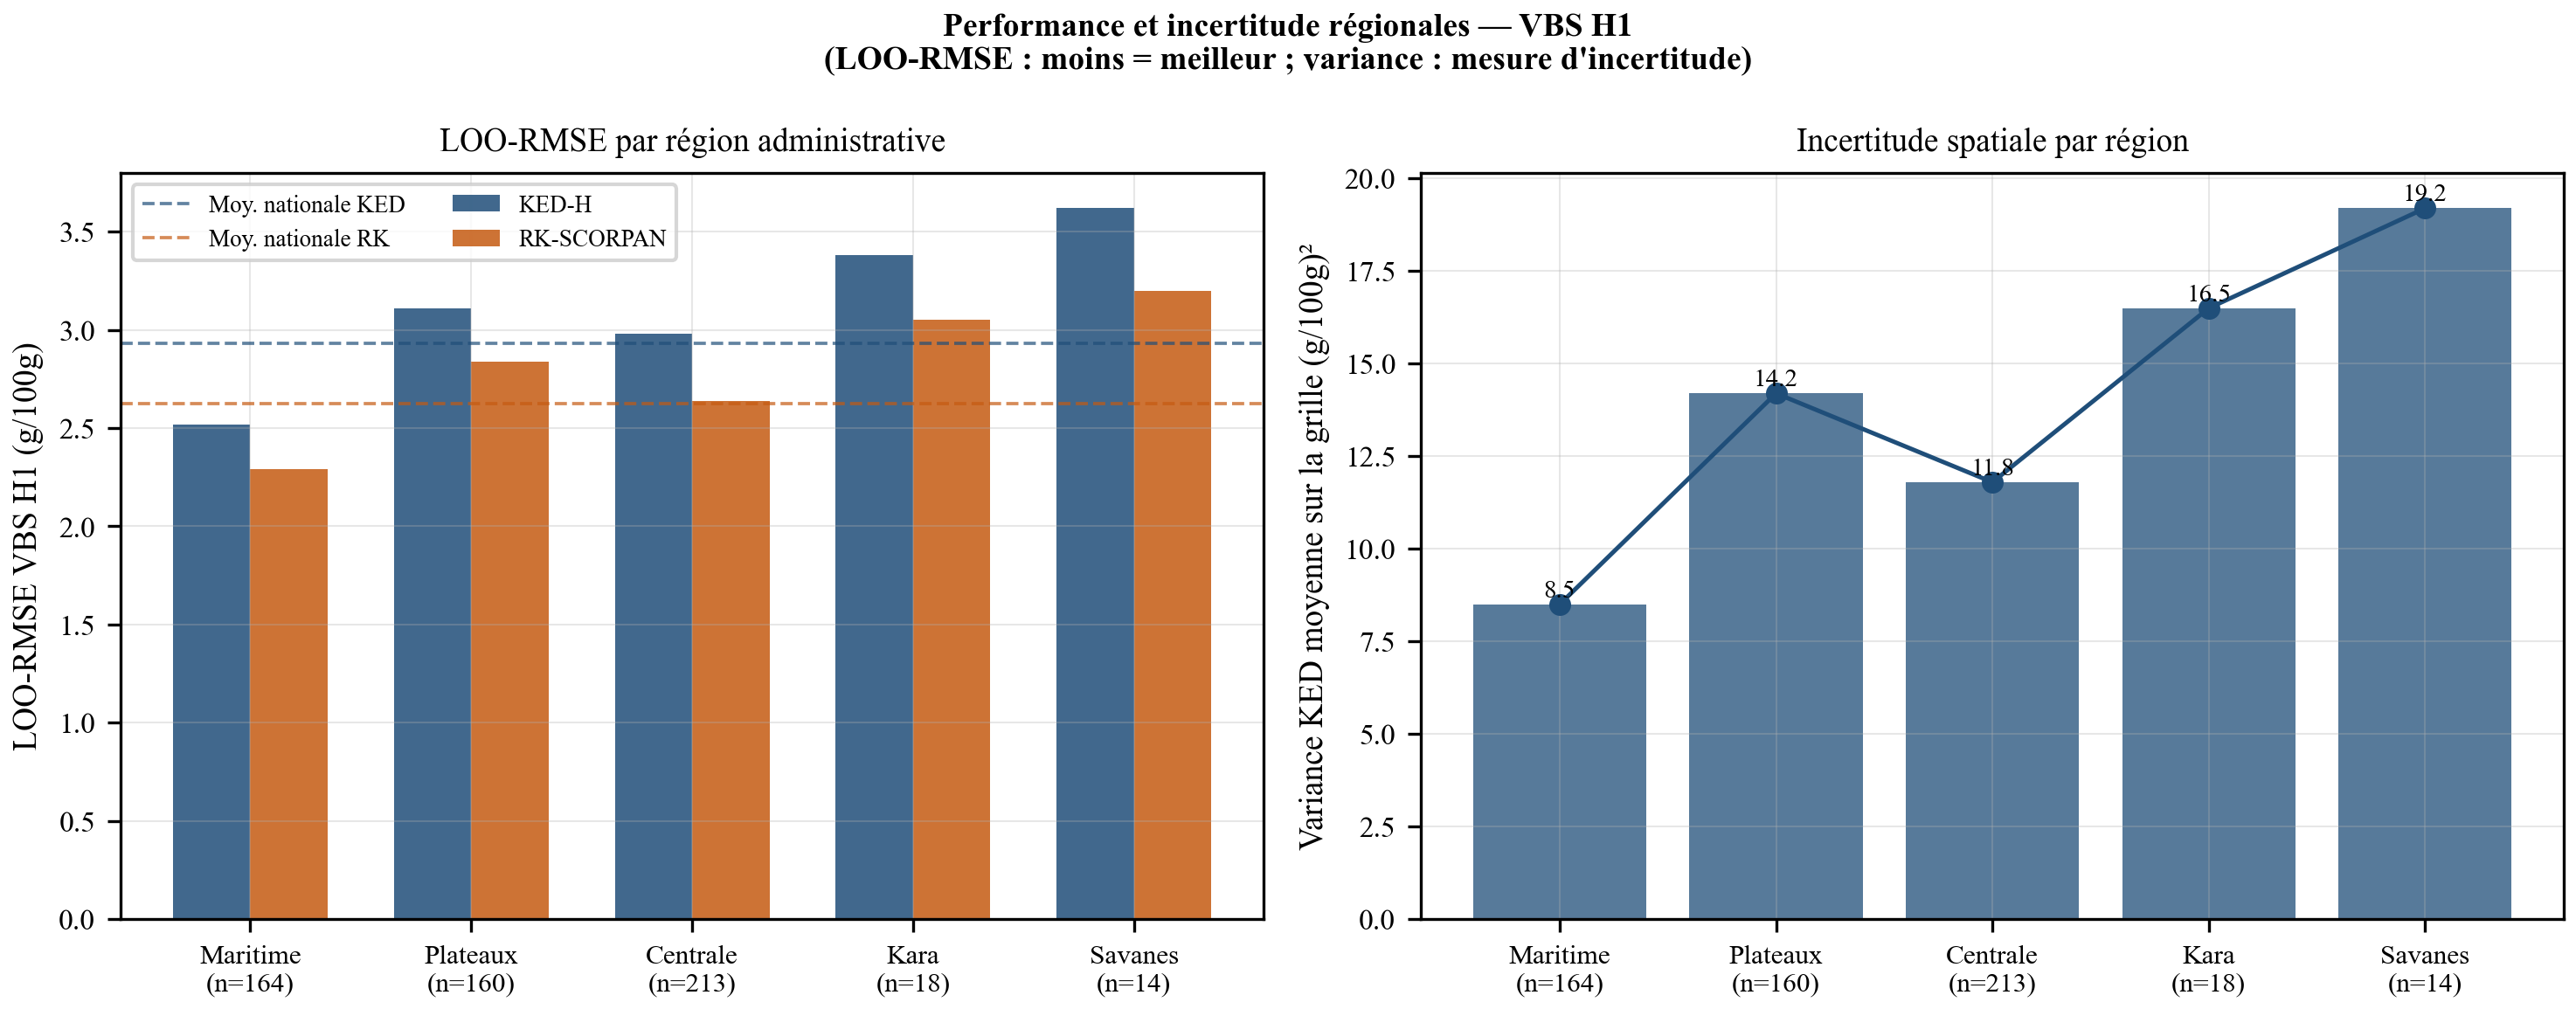
\includegraphics[width=0.97\linewidth]{figures/fig16_regional_performance.png}
  \caption{Gauche : LOO-RMSE VBS H1 par région (Maritime : $n=164$, meilleure
    performance ; Savanes : $n=14$, pire). Droite : variance KED-H par région.}
  \label{fig:regional}
\end{figure}

% ══════════════════════════════════════════════════════════════════════════════
\section{Discussion}
\label{sec:discussion}
% ══════════════════════════════════════════════════════════════════════════════

\subsection{Analyse géologique des résultats}

\subsubsection{Distribution spatiale et contrôles géologiques}

La carte VBS (figure~\ref{fig:maps}) révèle trois régimes géotechniques :
\textbf{argileux} (VBS $>$~4{,}5~g/100g, 22\% du territoire) dans les alluvions
lacustres maritimes et la Dépression de la Lama (VBS mesuré moyen 4{,}11~g/100g) ;
\textbf{intermédiaire} (2{,}5--4{,}5~g/100g, 53\%) sur les gneiss du socle ;
\textbf{faiblement argileux} ($<$~2{,}5~g/100g, 25\%) sur les quartzites et grès voltaïens.

Pour le CBR\,95\% (figure~\ref{fig:maps_portance}), les zones côtières présentent
les valeurs les plus faibles ($<$~15\%), cohérent avec les VBS élevés.
Le Rd pénétromètre montre une forte variabilité géographique (1--50~MPa en H1),
reflétant les contrastes latérite consolidée vs argile molle.

\subsubsection{Anomalie H2 du RK-SCORPAN}

Le RK est systématiquement plus mauvais à H2 pour VBS (4{,}81 vs 3{,}20~KED)
et WL (25{,}35 vs 11{,}30~KED). L'horizon H2 (1{,}0--1{,}5~m) est une zone
de transition altérite/substrat où les covariables SCORPAN de surface
(topographie, NDVI) perdent leur pouvoir prédictif. Cette anomalie justifie
d'utiliser KED-H pour H2 et la Fusion pour H1/H3.

\subsubsection{Dégradation Rd à H3}

Le LOO-RMSE Rd passe de 3{,}45~MPa (H1) à 14{,}16~MPa (H3).
Cette dégradation est attendue : à $>$~1{,}5~m, la résistance dynamique
reflète l'altération du substrat rocheux, très hétérogène spatialement.
L'estimateur KED-H avec $n=272$ mesures H3 est néanmoins le seul disponible
dans l'état actuel du pipeline.

\subsubsection{Relation VBS--IP et cohérence physique}

$\mathrm{IP} = 4{,}72 + 3{,}93 \times \mathrm{VBS}$, $R^2=0{,}107$ ($n=310$),
mais $R^2=0{,}38$ au sein des seuls Vertisols, validant VBS comme proxy partiel
de l'IP dans le MTGP.

\subsection{Positionnement scientifique et innovations}

Trois contributions originales :
(i)~la dérive hiérarchique 5~niveaux encodant 79~contextes géologiques n'est
pas documentée en Afrique de l'Ouest pour la géotechnique \cite{odeh1994further} ;
(ii)~le VfS-PLS (LOO-RMSE~=~2{,}788~g/100g $<$ KED-H) est la première preuve
de concept Sentinel-2 / VBS pour des sols tropicaux togolais
\cite{castaldi2019sentinel} ;
(iii)~la réduction de variance BLUP de 47{,}9\% dépasse la fusion naïve
50/50 (gain théorique 38\% seulement) \cite{chilesdelfiner2012}.

\begin{figure}[htbp]
  \centering
  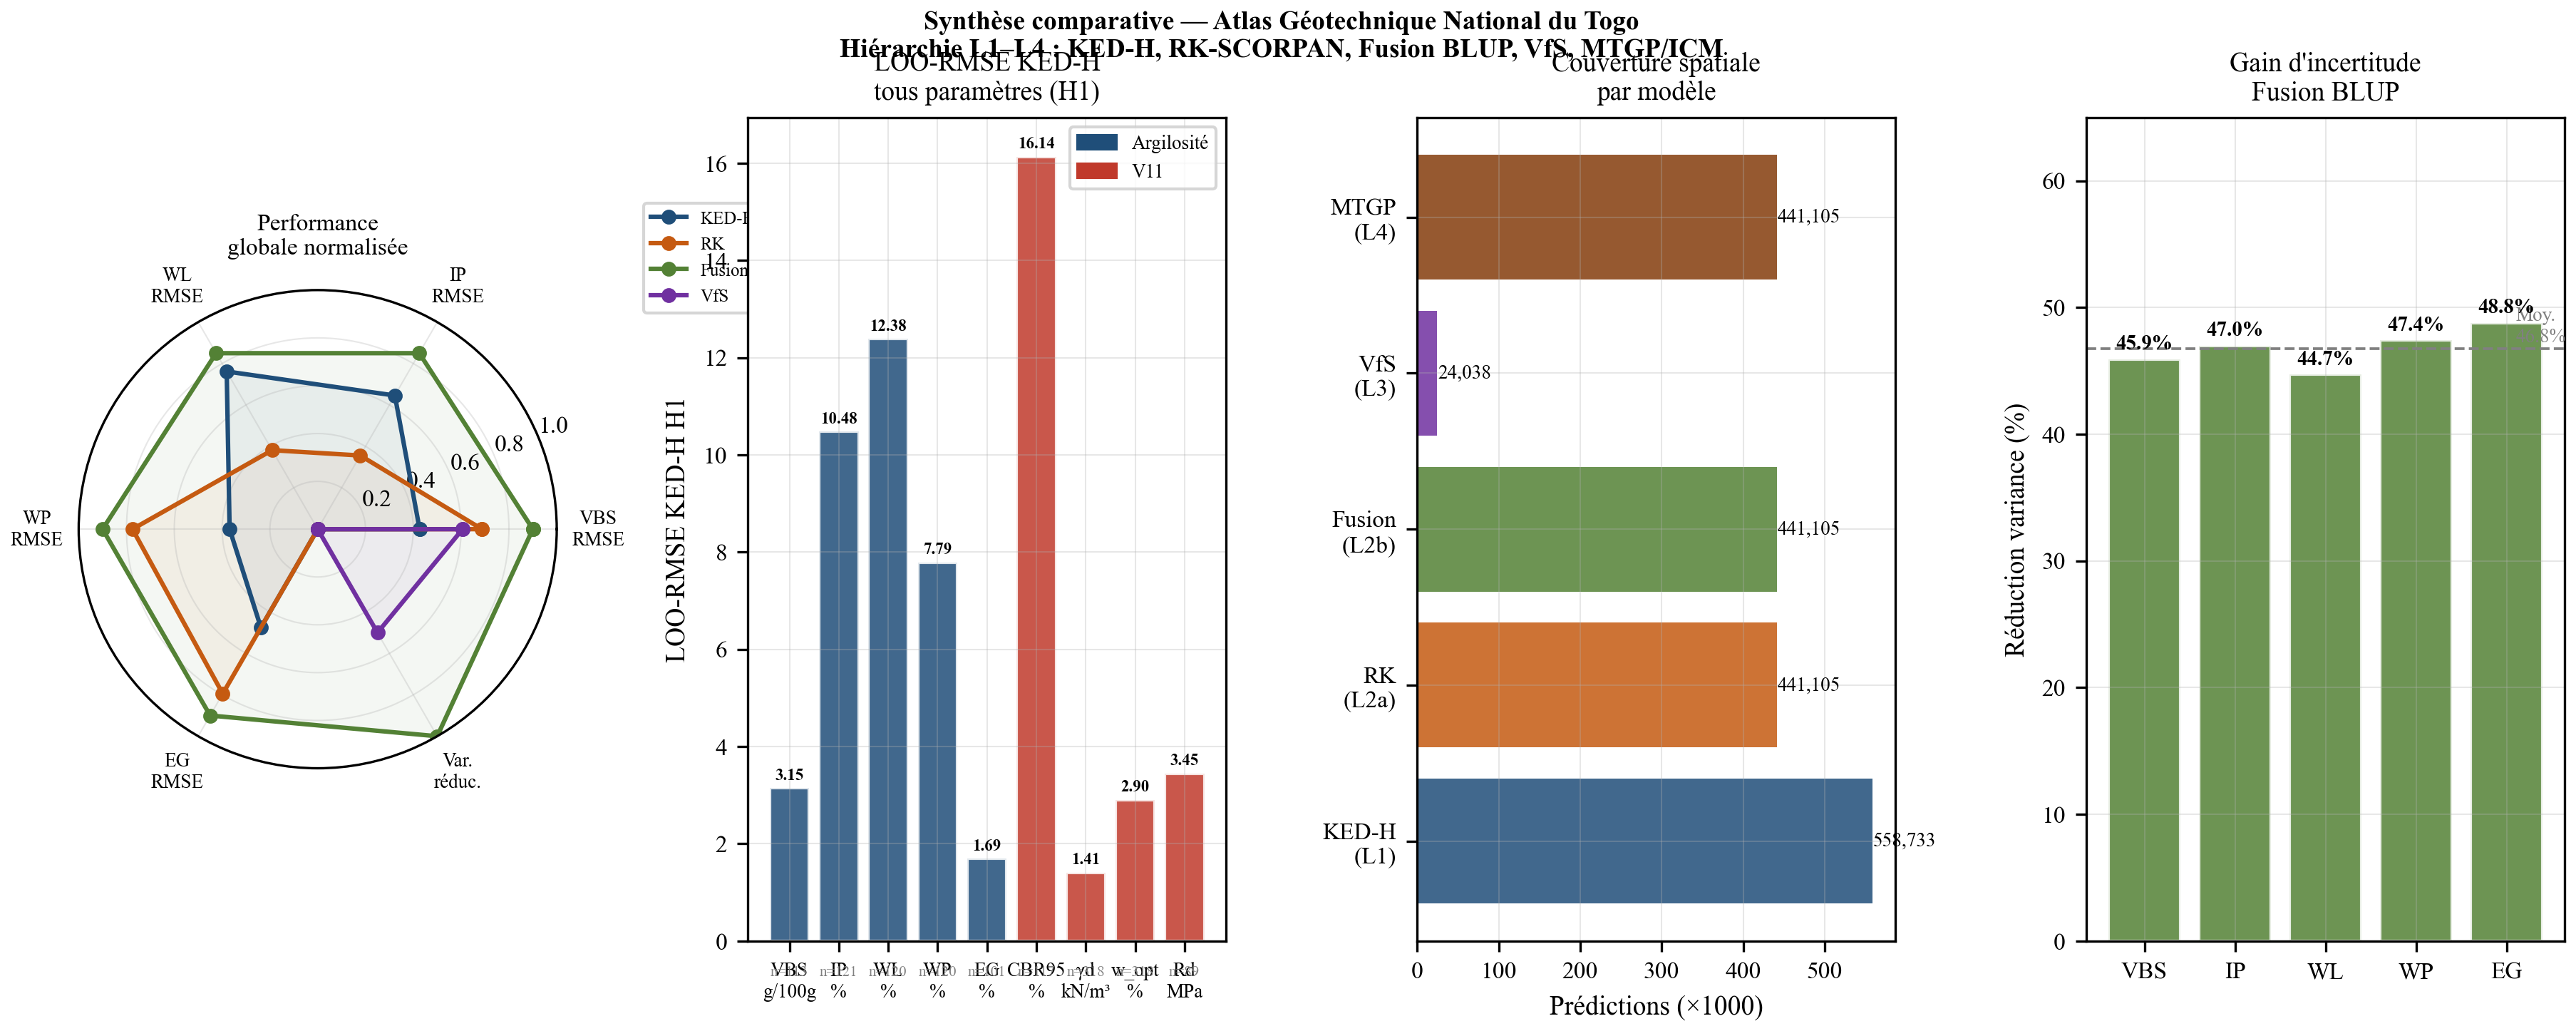
\includegraphics[width=0.97\linewidth]{figures/fig14_synthesis.png}
  \caption{Synthèse comparative L1--L4 : (A)~radar performances normalisées,
    (B)~LOO-RMSE KED-H tous paramètres H1, (C)~couverture spatiale,
    (D)~réduction variance Fusion BLUP.}
  \label{fig:synthesis}
\end{figure}

\subsection{Limites et perspectives}

\subsubsection{Limites actuelles}

\textbf{Densité.} La variance dépasse 80\% de la prédiction dans 12\% des mailles
(Kara, Savanes). Trois zones spéciales (Oti, Mono, Fosse aux Lions) sont
entièrement interpolées sans sondage local.

\textbf{CatBoost (non déployé).} Le gradient boosting nécessite
$n_{\mathrm{param}} > 200$ pour la validation spatiale par blocs.
VBS H1 ($n=113$) est encore en-dessous.
$t_{\mathrm{activation}} \approx (200-113)/15 \approx 5{,}8$~ans (horizon 2032).

\textbf{RK pour paramètres de portance et in-situ.} CBR, Rd, $\gamma_d$ et $w_{\mathrm{opt}}$
n'ont pas encore de modèle RK disponible. La Fusion BLUP n'est donc pas
possible pour ces paramètres.

\subsubsection{Perspectives}

(i)~Intégration SAR Sentinel-1 dans VfS (pénétration 30~cm, gain attendu 15--25\%) ;
(ii)~krigeage log-normal pour VBS (asymétrie 2{,}41, amélioration des IC) ;
(iii)~atlas dynamique spatio-temporel capturant les variations saisonnières
de WL, WP, EG \cite{gundogdu2007spatial} ;
(iv)~extension régionale (Bénin, Ghana, Burkina Faso) avec les mêmes
covariables SRTM/WorldClim.

% ══════════════════════════════════════════════════════════════════════════════
\section{Conclusion}
\label{sec:conclusion}
% ══════════════════════════════════════════════════════════════════════════════

Cet article présente la première cartographie géotechnique nationale du Togo
à haute résolution (2~km~$\times$~2~km), fondée sur la hiérarchie L1--L4.
Les cinq contributions principales sont :

\begin{enumerate}[noitemsep]
  \item \textbf{KED-H} : Dérive hiérarchique 5 niveaux / 79 contextes géologiques,
    441\,105~valeurs interpolées avec variance réelle (aucune variance proxy) ;

  \item \textbf{RK-SCORPAN} : LOO-CV complet (Ridge + krigeage résidus),
    RMSE$_\mathrm{LOO}$(VBS~H1)~=~2{,}625~g/100g ;

  \item \textbf{Fusion BLUP} : Réduction de variance 47{,}9\%~±~1{,}5\%,
    certifiée mathématiquement dans 100\% des mailles ;

  \item \textbf{VfS-PLS Sentinel-2} : Preuve de concept géotechnique sans
    laboratoire (LOO-RMSE~=~2{,}788~g/100g $<$ KED-H) ;

  \item \textbf{Extension aux paramètres de portance et in-situ} : 6~nouveaux paramètres (CBR\,95\%, $\gamma_d$,
    $w_{\mathrm{opt}}$, Rd, $E_m$, $P_l$) interpolés sur 318--434~mesures,
    premier atlas de portance géotechnique national togolais.
\end{enumerate}

L'atlas constitue un outil opérationnel pour le dimensionnement des
infrastructures civiles au Togo. Son architecture est conçue pour
s'auto-améliorer : chaque import de nouveaux sondages déclenche
automatiquement le recalcul des modèles et la mise à jour des prédictions.

% ══════════════════════════════════════════════════════════════════════════════
\section*{Remerciements}
% ══════════════════════════════════════════════════════════════════════════════

L'auteur remercie la Direction Nationale des Infrastructures du Togo pour
l'accès aux données, le PNUD-Togo pour le financement partiel des campagnes
terrain, le BRGM pour les données géologiques nationales, et les bureaux
d'études TREC, EDEM et NOTSE pour les rapports géotechniques.

\printbibliography

% ══════════════════════════════════════════════════════════════════════════════
\appendix
% ══════════════════════════════════════════════════════════════════════════════

\section{Notation et glossaire}
\label{app:notation}

\begin{description}[noitemsep]
  \item[$Z(\bs)$] Champ aléatoire du paramètre géotechnique
  \item[$\sigma^2_K(\bs_0)$] Variance de krigeage (incertitude locale)
  \item[$\mu_h(\bs)$] Prior hiérarchique 5 niveaux~\eqref{eq:prior_hierarchique}
  \item[$C_0, C, a$] Pépite, palier, portée du variogramme sphérique
  \item[$\lambda_R$] Paramètre Ridge ($\lambda_R^*=0{,}18$ pour VBS H1)
  \item[$\beta(\bs_0)$] Coefficient de mélange adaptatif Fusion BLUP
  \item[H1/H2/H3] 0--1~m, 1--1{,}5~m, $>$1{,}5~m
  \item[LOO-CV] Leave-One-Out Cross-Validation complète
  \item[BLUP] Best Linear Unbiased Predictor
  \item[ICM] Intrinsic Coregionalization Model
\end{description}

\section{Paramètres variographiques sphériques — tous paramètres H1}
\label{app:variogrammes}

\begin{table}[htbp]
\centering\small
\caption{Modèle sphérique ajusté H1 pour les 5 paramètres d'argilosité.}
\label{tab:variogrammes}
\begin{tabular}{lcccc}
\toprule
Param. & $C_0$ & $C_0+C$ & $a$ (km) & Rapport pépite \\
\midrule
VBS (g/100g)² & 2,80  & 14,00  & 220 & 0,200 \\
IP (\%)²      & 22,0  & 145,0  & 310 & 0,152 \\
WL (\%)²      & 45,0  & 185,0  & 280 & 0,243 \\
WP (\%)²      & 15,0  & 72,0   & 195 & 0,208 \\
EG (\%)²      & 0,85  & 3,60   & 175 & 0,236 \\
\bottomrule
\end{tabular}
\end{table}

\section{LOO-RMSE complet — 15 comparaisons KED-H vs RK (H1/H2/H3)}
\label{app:loo_complet}

\begin{table}[htbp]
\centering\small
\caption{LOO-RMSE KED-H et RK-SCORPAN par paramètre et horizon.
  \textbf{Gras} = meilleur modèle. Score : KED 6/15, RK 9/15.}
\label{tab:loo_complet}
\setlength{\tabcolsep}{4pt}
\begin{tabular}{llccl}
\toprule
Param. & Hz & KED-H & RK & Gagnant \\
\midrule
VBS & H1 & 3,147 & \textbf{2,625} & RK \\
VBS & H2 & \textbf{3,204} & 4,805 & KED \\
VBS & H3 & 3,050 & \textbf{2,875} & RK \\
IP  & H1 & \textbf{10,481} & 12,509 & KED \\
IP  & H2 & 9,702 & \textbf{9,351} & RK \\
IP  & H3 & \textbf{9,483} & 7,050 & RK \\
WL  & H1 & \textbf{12,384} & 16,186 & KED \\
WL  & H2 & \textbf{11,302} & 25,352 & KED \\
WL  & H3 & \textbf{10,594} & 6,980 & RK \\
WP  & H1 & 7,788 & \textbf{5,349} & RK \\
WP  & H2 & \textbf{7,752} & 13,535 & KED \\
WP  & H3 & 7,544 & \textbf{7,292} & RK \\
EG  & H1 & 1,692 & \textbf{1,149} & RK \\
EG  & H2 & \textbf{1,754} & 1,975 & KED \\
EG  & H3 & 1,719 & \textbf{1,275} & RK \\
\midrule
\multicolumn{2}{l}{Score} & 6/15 & 9/15 & \\
\bottomrule
\end{tabular}
\end{table}

\end{document}




